\documentclass[11pts,a4paper,amsmath,amssymb,floatfix]{book}

%\usepackage[gather]{chapterbib}

\usepackage{graphicx,wrapfig}% Include figure files
%\usepackage{dcolumn,enumerate}% Align table columns on decimal point
\usepackage{enumerate}% Align table columns on decimal point
\usepackage{bm,dpfloat}% bold math
\usepackage[pdftex,bookmarks,colorlinks=true,urlcolor=rltblue,citecolor=blue]{hyperref}
\usepackage{amsfonts,amsmath,amsthm,amssymb,stmaryrd,indentfirst}
\usepackage{times,psfrag,pdfpages}
%\usepackage{natbib} 
\usepackage{color}
\usepackage{units}
\usepackage{rotating}
\usepackage{multirow}


%\usepackage{algorithm}
\usepackage[linesnumbered,lined,boxed,commentsnumbered]{algorithm2e}
%[ruled,vlined][linesnumbered,lined,boxed,commentsnumbered]

\usepackage[noend]{algpseudocode}
\makeatletter
\def\BState{\State\hskip-\ALG@thistlm}
\makeatother

\usepackage{pifont}
\usepackage{subfigure}
\usepackage{subeqnarray}
\usepackage{ifthen}

\usepackage{pgfplots}
\pgfplotsset{every axis/.append style={
                    axis x line=middle,    % put the x axis in the middle
                    axis y line=middle,    % put the y axis in the middle
                    axis line style={<->}, % arrows on the axis
                    xlabel={$x$},          % default put x on x-axis
                    ylabel={$y$},          % default put y on y-axis
                }}



\usepackage{supertabular}
\usepackage{moreverb}
\usepackage{fancyvrb}
\usepackage{listings}
\usepackage{palatino}
%\usepackage{doi}
\usepackage{longtable}
\usepackage{float}
\usepackage{perpage}
\MakeSorted{figure}
%\usepackage{pdflscape}
\usepackage{framed}
\definecolor{shadecolor}{gray}{0.9}

% Appendix allows the inclusion of a line for "appendices", which otherwise won't get the right page number. You must
% use the [toc] option.
%\usepackage[toc]{appendix}

\definecolor{rltblue}{rgb}{0,0,0.75}

%\usepackage{natbib}
\usepackage{fancyhdr} %%%%
\pagestyle{fancy}%%%%
% with this we ensure that the chapter and section
% headings are in lowercase
%%%%\renewcommand{\chaptermark}[1]{\markboth{#1}{}}
\renewcommand{\sectionmark}[1]{\markright{\thesection\ #1}}
\fancyhf{} %delete the current section for header and footer
%\fancyhead[LE,RO]{\bfseries\thepage}
%\fancyfoot[LE,RO]{\bfseries\thepage}
\fancyhead[LO]{\bfseries\rightmark}
\fancyhead[RE]{\bfseries\leftmark}
\renewcommand{\headrulewidth}{0.5pt}
% make space for the rule
\fancypagestyle{plain}{%
\fancyhead{} %get rid of the headers on plain pages
\renewcommand{\headrulewidth}{0pt} % and the line
}

\def\newblock{\hskip .11em plus .33em minus .07em}
\usepackage{color}

\theoremstyle{definition}
\newtheorem{exmp}{Example}[chapter]

% For theorems
\newtheorem{theorem}{Theorem}[section]
\newtheorem{corollary}{Corollary}[theorem]
\newtheorem{lemma}[theorem]{Lemma}

\usepackage{makeidx}
\makeindex

\setlength\textwidth      {16.cm}
\setlength\textheight     {23.0cm}
\setlength\oddsidemargin  {-0.3cm}
\setlength\evensidemargin {0.3cm}

\setlength\headheight{14.49998pt} 
\setlength\topmargin{0.0cm}
\setlength\headsep{1.cm}
\setlength\footskip{-0.cm}
\setlength\parskip{0pt}

%%%
%%% Headers and Footers
%\lhead[\text{\small{WORK IN PROGRESS}}] {\text{\small{ICON/AMCG}}} 
%-\lhead[] {\text{\small{ICON/AMCG}}} 
%-\chead[\text{\small{FETCH Manual}}]  {\text{\small{FETCH Manual}}} %{\text{\small{JAERI Analysis Report Issue}}}
%-\rhead[\text{\small{Commercial-in Confidence}}]{}
\cfoot[\thepage]{\thepage}
%-\rfoot[]{}%{\text{\small{\today}}}
%\cfoot[\text{\small{\today}}]{}% {\text{\small{\today}}}
%\cfoot[\text{\small{January 2006}}] {\text{\small{January 2006}}}
%-\lfoot []{}%{\text{\small{Numerical Analysis}}}
%-\renewcommand{\headrulewidth}{0.8pt}

%%%
%%% space between lines
%%%
\renewcommand{\baselinestretch}{1.5}

\newenvironment{VarDescription}[1]%
  {\begin{list}{}{\renewcommand{\makelabel}[1]{\textbf{##1:}\hfil}%
    \settowidth{\labelwidth}{\textbf{#1:}}%
    \setlength{\leftmargin}{\labelwidth}\addtolength{\leftmargin}{\labelsep}}}%
  {\end{list}}

%%%%%%%%%%%%%%%%%%%%%%%%%%%%%%%%%%%%%%%%%%%
%%%%%%                              %%%%%%%
%%%%%%      NOTATION SECTION        %%%%%%%
%%%%%%                              %%%%%%%
%%%%%%%%%%%%%%%%%%%%%%%%%%%%%%%%%%%%%%%%%%%

% Text abbreviations.
\newcommand{\ie}{{\em{i.e., }}}
\newcommand{\eg}{{\em{e.g., }}}
\newcommand{\cf}{{\em{cf., }}}
\newcommand{\fetch}{FETCH }
\newcommand{\fmips}{FETCH-MIPS }
\newcommand{\bw}{B$\$$W }
\newcommand{\fluidity}{Fluidity }
\newcommand{\event}{{EVENT }}
\newcommand{\gem}{GEM }
\newcommand{\radiant}{RADIANT }
\newcommand{\wrt}{with respect to}
\newcommand{\lhs}{left hand side}
\newcommand{\rhs}{right hand side}
\newcommand{\vv}{V$\&$V }
\newcommand{\cse}{CS$\&$E }
\newcommand{\amcg}{\href{http://amcg.ese.ic.ac.uk}{AMCG }}
% Commands definining mathematical notation.

% This is for quantities which are physically vectors.
\renewcommand{\vec}[1]{{\mbox{\boldmath$#1$}}}
% Physical rank 2 tensors
\newcommand{\tensor}[1]{\overline{\overline{#1}}}
% This is for vectors formed of the value of a quantity at each node.
\newcommand{\dvec}[1]{\underline{#1}}
% This is for matrices in the discrete system.
\newcommand{\mat}[1]{\mathrm{#1}}


\DeclareMathOperator{\sgn}{sgn}

%\newcommand\qed{\hfill\mbox{$\Box$}}
\newcommand{\re}{{\mathrm{I}\hspace{-0.2em}\mathrm{R}}}
\newcommand{\inner}[2]{\langle#1,#2\rangle}
\renewcommand\leq{\leqslant}
\renewcommand\geq{\geqslant}
\renewcommand\le{\leqslant}
\renewcommand\ge{\geqslant}
\renewcommand\epsilon{\varepsilon}
\newcommand\eps{\varepsilon}
\newcommand{\bmF}{\vec{F}}
\newcommand{\bmphi}{\vec{\phi}}
\newcommand{\bmn}{\vec{n}}
\newcommand{\bmns}{{\textrm{\scriptsize{\boldmath $n$}}}}
\newcommand{\bmi}{\vec{i}}
\newcommand{\bmj}{\vec{j}}
\newcommand{\bmk}{\vec{k}}
\newcommand{\bmx}{\vec{x}}
\newcommand{\bmu}{\vec{u}}
\newcommand{\bmv}{\vec{v}}
\newcommand{\bmr}{\vec{r}}
\newcommand{\bma}{\vec{a}}
\newcommand{\bmg}{\vec{g}}
\newcommand{\bmU}{\vec{U}}
\newcommand{\bmI}{\vec{I}}
\newcommand{\bmq}{\vec{q}}
\newcommand{\bmT}{\vec{T}}
\newcommand{\bmM}{\vec{M}}
\newcommand{\bmtau}{\vec{\tau}}
\newcommand{\bmOmega}{\vec{\Omega}}
\newcommand{\pp}{\partial}
\newcommand{\kaptens}{\tensor{\kappa}}
\newcommand{\tautens}{\tensor{\tau}}
\newcommand{\sigtens}{\tensor{\sigma}}
\newcommand{\etens}{\tensor{\dot\epsilon}}
\newcommand{\ktens}{\tensor{k}}
\newcommand{\half}{{\textstyle \frac{1}{2}}}
\newcommand{\tote}{E}
\newcommand{\inte}{e}
\newcommand{\strt}{\dot\epsilon}
\newcommand{\modu}{|\bmu|}
% Derivatives
\renewcommand{\d}{\mathrm{d}}
\newcommand{\D}{\mathrm{D}}
\newcommand{\ddx}[2][x]{\frac{\d#2}{\d#1}}
\newcommand{\ddxx}[2][x]{\frac{\d^2#2}{\d#1^2}}
\newcommand{\ddt}[2][t]{\frac{\d#2}{\d#1}}
\newcommand{\ddtt}[2][t]{\frac{\d^2#2}{\d#1^2}}
\newcommand{\ppx}[2][x]{\frac{\partial#2}{\partial#1}}
\newcommand{\ppxx}[2][x]{\frac{\partial^2#2}{\partial#1^2}}
\newcommand{\ppt}[2][t]{\frac{\partial#2}{\partial#1}}
\newcommand{\pptt}[2][t]{\frac{\partial^2#2}{\partial#1^2}}
\newcommand{\DDx}[2][x]{\frac{\D#2}{\D#1}}
\newcommand{\DDxx}[2][x]{\frac{\D^2#2}{\D#1^2}}
\newcommand{\DDt}[2][t]{\frac{\D#2}{\D#1}}
\newcommand{\DDtt}[2][t]{\frac{\D^2#2}{\D#1^2}}
% Norms
\newcommand{\Ltwo}{\ensuremath{L_2} }
% Basis functions
\newcommand{\Qone}{\ensuremath{Q_1} }
\newcommand{\Qtwo}{\ensuremath{Q_2} }
\newcommand{\Qthree}{\ensuremath{Q_3} }
\newcommand{\QN}{\ensuremath{Q_N} }
\newcommand{\Pzero}{\ensuremath{P_0} }
\newcommand{\Pone}{\ensuremath{P_1} }
\newcommand{\Ptwo}{\ensuremath{P_2} }
\newcommand{\Pthree}{\ensuremath{P_3} }
\newcommand{\PN}{\ensuremath{P_N} }
\newcommand{\Poo}{\ensuremath{P_1P_1} }
\newcommand{\PoDGPt}{\ensuremath{P_{-1}P_2} }

\newcommand{\metric}{\tensor{M}}
\newcommand{\configureflag}[1]{\texttt{#1}}

% Units
\newcommand{\m}[1][]{\unit[#1]{m}}
\newcommand{\km}[1][]{\unit[#1]{km}}
\newcommand{\s}[1][]{\unit[#1]{s}}
\newcommand{\invs}[1][]{\unit[#1]{s}\ensuremath{^{-1}}}
\newcommand{\ms}[1][]{\unit[#1]{m\ensuremath{\,}s\ensuremath{^{-1}}}}
\newcommand{\mss}[1][]{\unit[#1]{m\ensuremath{\,}s\ensuremath{^{-2}}}}
\newcommand{\K}[1][]{\unit[#1]{K}}
\newcommand{\PSU}[1][]{\unit[#1]{PSU}}
\newcommand{\Pa}[1][]{\unit[#1]{Pa}}
\newcommand{\kg}[1][]{\unit[#1]{kg}}
\newcommand{\rads}[1][]{\unit[#1]{rad\ensuremath{\,}s\ensuremath{^{-1}}}}
\newcommand{\kgmm}[1][]{\unit[#1]{kg\ensuremath{\,}m\ensuremath{^{-2}}}}
\newcommand{\kgmmm}[1][]{\unit[#1]{kg\ensuremath{\,}m\ensuremath{^{-3}}}}
\newcommand{\Nmm}[1][]{\unit[#1]{N\ensuremath{\,}m\ensuremath{^{-2}}}}

% Dimensionless numbers
\newcommand{\dimensionless}[1]{\mathrm{#1}}
\renewcommand{\Re}{\dimensionless{Re}}
\newcommand{\Ro}{\dimensionless{Ro}}
\newcommand{\Fr}{\dimensionless{Fr}}
\newcommand{\Bu}{\dimensionless{Bu}}
\newcommand{\Ri}{\dimensionless{Ri}}
\renewcommand{\Pr}{\dimensionless{Pr}}
\newcommand{\Pe}{\dimensionless{Pe}}
\newcommand{\Ek}{\dimensionless{Ek}}
\newcommand{\Gr}{\dimensionless{Gr}}
\newcommand{\Ra}{\dimensionless{Ra}}
\newcommand{\Sh}{\dimensionless{Sh}}
\newcommand{\Sc}{\dimensionless{Sc}}


% Journals
\newcommand{\IJHMT}{{\it International Journal of Heat and Mass Transfer}}
\newcommand{\NED}{{\it Nuclear Engineering and Design}}
\newcommand{\ICHMT}{{\it International Communications in Heat and Mass Transfer}}
\newcommand{\NET}{{\it Nuclear Engineering and Technology}}
\newcommand{\HT}{{\it Heat Transfer}}   
\newcommand{\IJHT}{{\it International Journal for Heat Transfer}}


\newcommand{\frc}{\displaystyle\frac}
\newcommand{\red}{\textcolor{red}}
\newcommand{\blue}{\textcolor{blue}}
\newcommand{\green}{\textcolor{green}}
\newcommand{\purple}{\textcolor{purple}}
\newcommand{\PNDG}[3][error]{P$_{#1}$DG-P$_{#2}$DG$_{#3}$}
\newcommand{\Partial}[3][error]{\left(\frc{\partial #1}{\partial #2}\right)_{#3}}
%{P$_{#1}$DG-P$_{#2}$DG}%$_{#3}$}

%%%%%%%%%%%%%%%%%%%%%%%%%%%%%%%%%%%%%%%%%%%
%%%%%%                              %%%%%%%
%%%%%% END OF THE NOTATION SECTION  %%%%%%%
%%%%%%                              %%%%%%%
%%%%%%%%%%%%%%%%%%%%%%%%%%%%%%%%%%%%%%%%%%%

% Cause numbering of subsubsections. 
%\setcounter{secnumdepth}{8}
%\setcounter{tocdepth}{8}

\setcounter{secnumdepth}{4}%
\setcounter{tocdepth}{4}%

\newcounter{qcounter}
\newcounter{mcounter}
\includeonly{Module_01, Module_02}
%\includeonly{model_introduction, model_reservoir_equations, model_description}
\DeclareMathAlphabet{\mathpzc}{OT1}{pzc}{m}{it}

\begin{document}

\vspace{4cm}

\begin{titlepage}
\begin{center}
\bigskip

   
\includegraphics[width=15cm,clip]{./../FigBanner/UoAHorizBanner}

\bigskip
\vspace{3.5cm}

   {\bf{\Huge Fundamentals of Applied Thermodynamics }}

\bigskip
   {\bf{\huge Lecture Notes}}

\vspace{3.5cm}

\end{center}

\begin{tabular}{l c l}
{\bf{\large Author:}}                          &     & J.L.M.A. Gomes \\
%                                               &     & Environmental and Industrial Fluid Mechanics Group \\
                                               &     & School of Engineering \\
                                               &     & University of Aberdeen \\
\bigskip
{\bf{\large Date:}}                            &     &   \today\\
                                               &     &         \\
{\bf{\large Revision 1:}}                      &     &   \today\\
                                               &     &         \\
\end{tabular}
\vspace{3.5cm}

\bigskip

\bigskip




\end{titlepage}

\setcounter{page}{1}

\tableofcontents
\vfill

\pagebreak
\listoftables
\vfill
\pagebreak
\listoffigures
\vfill
\pagebreak

\part{Introduction and Review of Basic Concepts}
% Aberdeen style guide should be followed when using this
% layout. Their template powerpoint slide is used to extract the
% Aberdeen color and logo but is otherwise ignored (it has little or
% no formatting in it anyway).
%
% http://www.abdn.ac.uk/documents/style-guide.pdf

%%%%%%%%%%%%%%%%%%%% Document Class Settings %%%%%%%%%%%%%%%%%%%%%%%%%
% Pick if you want slides, or draft slides (no animations)
%%%%%%%%%%%%%%%%%%%%%%%%%%%%%%%%%%%%%%%%%%%%%%%%%%%%%%%%%%%%%%%%%%%%%%
%Normal document mode%
\documentclass[10pt,compress]{beamer}
%Draft or handout mode
%\documentclass[10pt,compress,handout]{beamer}
%\documentclass[10pt,compress,handout,ignorenonframetext]{beamer}

\renewcommand{\insertframenumber}{\theframenumber}
\renewcommand{\theframenumber}{\thesection-\arabic{framenumber}}
\renewcommand{\thesubsectionslide}{\thesection-\arabic{framenumber}}
\setbeamertemplate{headline}[text line]{This is frame: \insertframenumber}
\AtBeginSection{\setcounter{framenumber}{0}}

%%%%%%%%%%%%%%%%%%%% General Document settings %%%%%%%%%%%%%%%%%%%%%%%
% These settings must be set for each presentation
%%%%%%%%%%%%%%%%%%%%%%%%%%%%%%%%%%%%%%%%%%%%%%%%%%%%%%%%%%%%%%%%%%%%%%
\newcommand{\shortname}{jefferson.gomes@abdn.ac.uk}
\newcommand{\fullname}{Dr Jeff Gomes}
\institute{School of Engineering}
\newcommand{\emailaddress}{}%jefferson.gomes@abdn.ac.uk}
\newcommand{\logoimage}{../FigBanner/UoAHorizBanner}
\title{Engineering Thermodynamics (EG3521)}
\subtitle{Module 1: Introduction and Principles}
%\subtitle{Module 1.1: Review of Thermodynamics}
\date[2014-15]{2014-15}

%%%%%%%%%%%%%%%%%%%% Template settings %%%%%%%%%%%%%%%%%%%%%%%%%%%%%%%
% You shouldn't have to change below this line, unless you want to.
%%%%%%%%%%%%%%%%%%%%%%%%%%%%%%%%%%%%%%%%%%%%%%%%%%%%%%%%%%%%%%%%%%%%%%
\usecolortheme{whale}
\useoutertheme{infolines}

% Use the fading effect for items that are covered on the current
% slide.
\beamertemplatetransparentcovered

% We abuse the author command to place all of the slide information on
% the title page.
\author[\shortname]{%
  \fullname\\\ttfamily{\emailaddress}
}


%At the start of every section, put a slide indicating the contents of the current section.
\AtBeginSection[] {
  \begin{frame}
    \frametitle{Section Outline}
    \tableofcontents[currentsection]
  \end{frame}
}

% Allow the inclusion of movies into the Presentation! At present,
% only the Okular program is capable of playing the movies *IN* the
% presentation.
\usepackage{multimedia}
\usepackage{animate}

%% Handsout -- comment out the lines below to create handstout with 4 slides in a page with space for comments
\usepackage{handoutWithNotes}

\mode<handout>
{
\usepackage{pgf,pgfpages}

\pgfpagesdeclarelayout{2 on 1 boxed with notes}
{
\edef\pgfpageoptionheight{\the\paperheight} 
\edef\pgfpageoptionwidth{\the\paperwidth}
\edef\pgfpageoptionborder{0pt}
}
{
\setkeys{pgfpagesuselayoutoption}{landscape}
\pgfpagesphysicalpageoptions
    {%
        logical pages=4,%
        physical height=\pgfpageoptionheight,%
        physical width=\pgfpageoptionwidth,%
        last logical shipout=2%
    } 
\pgfpageslogicalpageoptions{1}
    {%
    border code=\pgfsetlinewidth{1pt}\pgfstroke,%
    scale=1,
    center=\pgfpoint{.25\pgfphysicalwidth}{.75\pgfphysicalheight}%
    }%
\pgfpageslogicalpageoptions{2}
    {%
    border code=\pgfsetlinewidth{1pt}\pgfstroke,%
    scale=1,
    center=\pgfpoint{.25\pgfphysicalwidth}{.25\pgfphysicalheight}%
    }%
\pgfpageslogicalpageoptions{3}
    {%
    border shrink=\pgfpageoptionborder,%
    resized width=.7\pgfphysicalwidth,%
    resized height=.5\pgfphysicalheight,%
    center=\pgfpoint{.75\pgfphysicalwidth}{.29\pgfphysicalheight},%
    copy from=3
    }%
\pgfpageslogicalpageoptions{4}
    {%
    border shrink=\pgfpageoptionborder,%
    resized width=.7\pgfphysicalwidth,%
    resized height=.5\pgfphysicalheight,%
    center=\pgfpoint{.75\pgfphysicalwidth}{.79\pgfphysicalheight},%
    copy from=4
    }%

\AtBeginDocument
    {
    \newbox\notesbox
    \setbox\notesbox=\vbox
        {
            \hsize=\paperwidth
            \vskip-1in\hskip-1in\vbox
            {
                \vskip1cm
                Notes\vskip1cm
                        \hrule width\paperwidth\vskip1cm
                    \hrule width\paperwidth\vskip1cm
                        \hrule width\paperwidth\vskip1cm
                    \hrule width\paperwidth\vskip1cm
                        \hrule width\paperwidth\vskip1cm
                    \hrule width\paperwidth\vskip1cm
                    \hrule width\paperwidth\vskip1cm
                    \hrule width\paperwidth\vskip1cm
                        \hrule width\paperwidth
            }
        }
        \pgfpagesshipoutlogicalpage{3}\copy\notesbox
        \pgfpagesshipoutlogicalpage{4}\copy\notesbox
    }
}
}

%\pgfpagesuselayout{2 on 1 boxed with notes}[letterpaper,border shrink=5mm]
%\pgfpagesuselayout{2 on 1 boxed with notes}[letterpaper,border shrink=5mm]

%%%%% Color settings
\usepackage{color}
%% The background color for code listings (i.e. example programs)
\definecolor{lbcolor}{rgb}{0.9,0.9,0.9}%
\definecolor{UoARed}{rgb}{0.64706, 0.0, 0.12941}
\definecolor{UoALight}{rgb}{0.85, 0.85, 0.85}
\definecolor{UoALighter}{rgb}{0.92, 0.92, 0.92}
\setbeamercolor{structure}{fg=UoARed} % General background and higlight color
\setbeamercolor{frametitle}{bg=black} % General color
\setbeamercolor{frametitle right}{bg=black} % General color
\setbeamercolor{block body}{bg=UoALighter} % For blocks
\setbeamercolor{structure}{bg=UoALight} % For blocks
% Rounded boxes for blocks
\setbeamertemplate{blocks}[rounded]

%%%%% Font settings
% Aberdeen requires the use of Arial in slides. We can use the
% Helvetica font as its widely available like so
% \usepackage{helvet}
% \renewcommand{\familydefault}{\sfdefault}
% But beamer already uses a sans font, so we will stick with that.

% The size of the font used for the code listings.
\newcommand{\goodsize}{\fontsize{6}{7}\selectfont}

% Extra math packages, symbols and colors. If you're using Latex you
% must be using it for formatting the math!
\usepackage{amscd,amssymb} \usepackage{amsfonts}
\usepackage[mathscr]{eucal} \usepackage{mathrsfs}
\usepackage{latexsym} \usepackage{amsmath} \usepackage{bm}
\usepackage{amsthm} \usepackage{textcomp} \usepackage{eurosym}
% This package provides \cancel{a} and \cancelto{a}{b} to "cancel"
% expressions in math.
\usepackage{cancel}

\usepackage{comment} 

% Get rid of font warnings as modern LaTaX installations have scalable
% fonts
\usepackage{type1cm} 

%\usepackage{enumitem} % continuous numbering throughout enumerate commands

% For exact placement of images/text on the cover page
\usepackage[absolute]{textpos}
\setlength{\TPHorizModule}{1mm}%sets the textpos unit
\setlength{\TPVertModule}{\TPHorizModule} 

% Source code formatting package
\usepackage{listings}%
\lstset{ backgroundcolor=\color{lbcolor}, tabsize=4,
  numberstyle=\tiny, rulecolor=, language=C++, basicstyle=\goodsize,
  upquote=true, aboveskip={1.5\baselineskip}, columns=fixed,
  showstringspaces=false, extendedchars=true, breaklines=false,
  prebreak = \raisebox{0ex}[0ex][0ex]{\ensuremath{\hookleftarrow}},
  frame=single, showtabs=false, showspaces=false,
  showstringspaces=false, identifierstyle=\ttfamily,
  keywordstyle=\color[rgb]{0,0,1},
  commentstyle=\color[rgb]{0.133,0.545,0.133},
  stringstyle=\color[rgb]{0.627,0.126,0.941}}

% Allows the inclusion of other PDF's into the final PDF. Great for
% attaching tutorial sheets etc.
\usepackage{pdfpages}
\setbeamercolor{background canvas}{bg=}  

% Remove foot note horizontal rules, they occupy too much space on the slide
\renewcommand{\footnoterule}{}

% Force the driver to fix the colors on PDF's which include mixed
% colorspaces and transparency.
\pdfpageattr {/Group << /S /Transparency /I true /CS /DeviceRGB>>}

% Include a graphics, reserve space for it but
% show it on the next frame.
% Parameters:
% #1 Which slide you want it on
% #2 Previous slides
% #3 Options to \includegraphics (optional)
% #4 Name of graphic
\newcommand{\reserveandshow}[4]{%
\phantom{\includegraphics<#2|handout:0>[#3]{#4}}%
\includegraphics<#1>[#3]{#4}%
}

\newcommand{\frc}{\displaystyle\frac}
\newcommand{\red}{\textcolor{red}}
\newcommand{\blue}{\textcolor{blue}}
\newcommand{\green}{\textcolor{green}}
\newcommand{\purple}{\textcolor{purple}}
 

\begin{document}

% Title page layout
\begin{frame}
  \titlepage
  \vfill%
  \begin{center}
    \includegraphics[clip,width=0.8\textwidth]{\logoimage}
  \end{center}
\end{frame}

% Table of contents
%\frame{ \frametitle{Slides Outline}
%  \tableofcontents
%}


%%%%%%%%%%%%%%%%%%%% The Presentation Proper %%%%%%%%%%%%%%%%%%%%%%%%%
% Fill below this line with \begin{frame} commands! It's best to
% always add the fragile option incase you're going to use the
% verbatim environment.
%%%%%%%%%%%%%%%%%%%%%%%%%%%%%%%%%%%%%%%%%%%%%%%%%%%%%%%%%%%%%%%%%%%%%%

%%%
%%% SECTION
%%%
\section{Introduction}

%%%
%%% Slide
%%%
\subsection{Motivation}
\begin{frame}
 \frametitle{Aims and Objectives}
  \begin{columns}
    \begin{column}[l]{0.6\linewidth}
     \begin{enumerate}[(a)]
      \item <2-> We aim to understand how energy evolves or is consumed in industrial- or environmental-based processes.
      \item <3-> In order to achieve this, we first must define the thermodynamic system and review the definition of:
       \begin{enumerate}[(i)]
        \item  Intensive and extensive properties;
        \item  Laws of thermodynamics;
        \item  Reversible and irreversible processes;
       \end{enumerate}
      \item <4->Finally, we should review applications of the \textcolor{red}{{\it First Law}}. 
     \end{enumerate}
    \end{column}
     \begin{column}[l]{0.4\linewidth}
      \begin{figure}%
        \begin{center}
          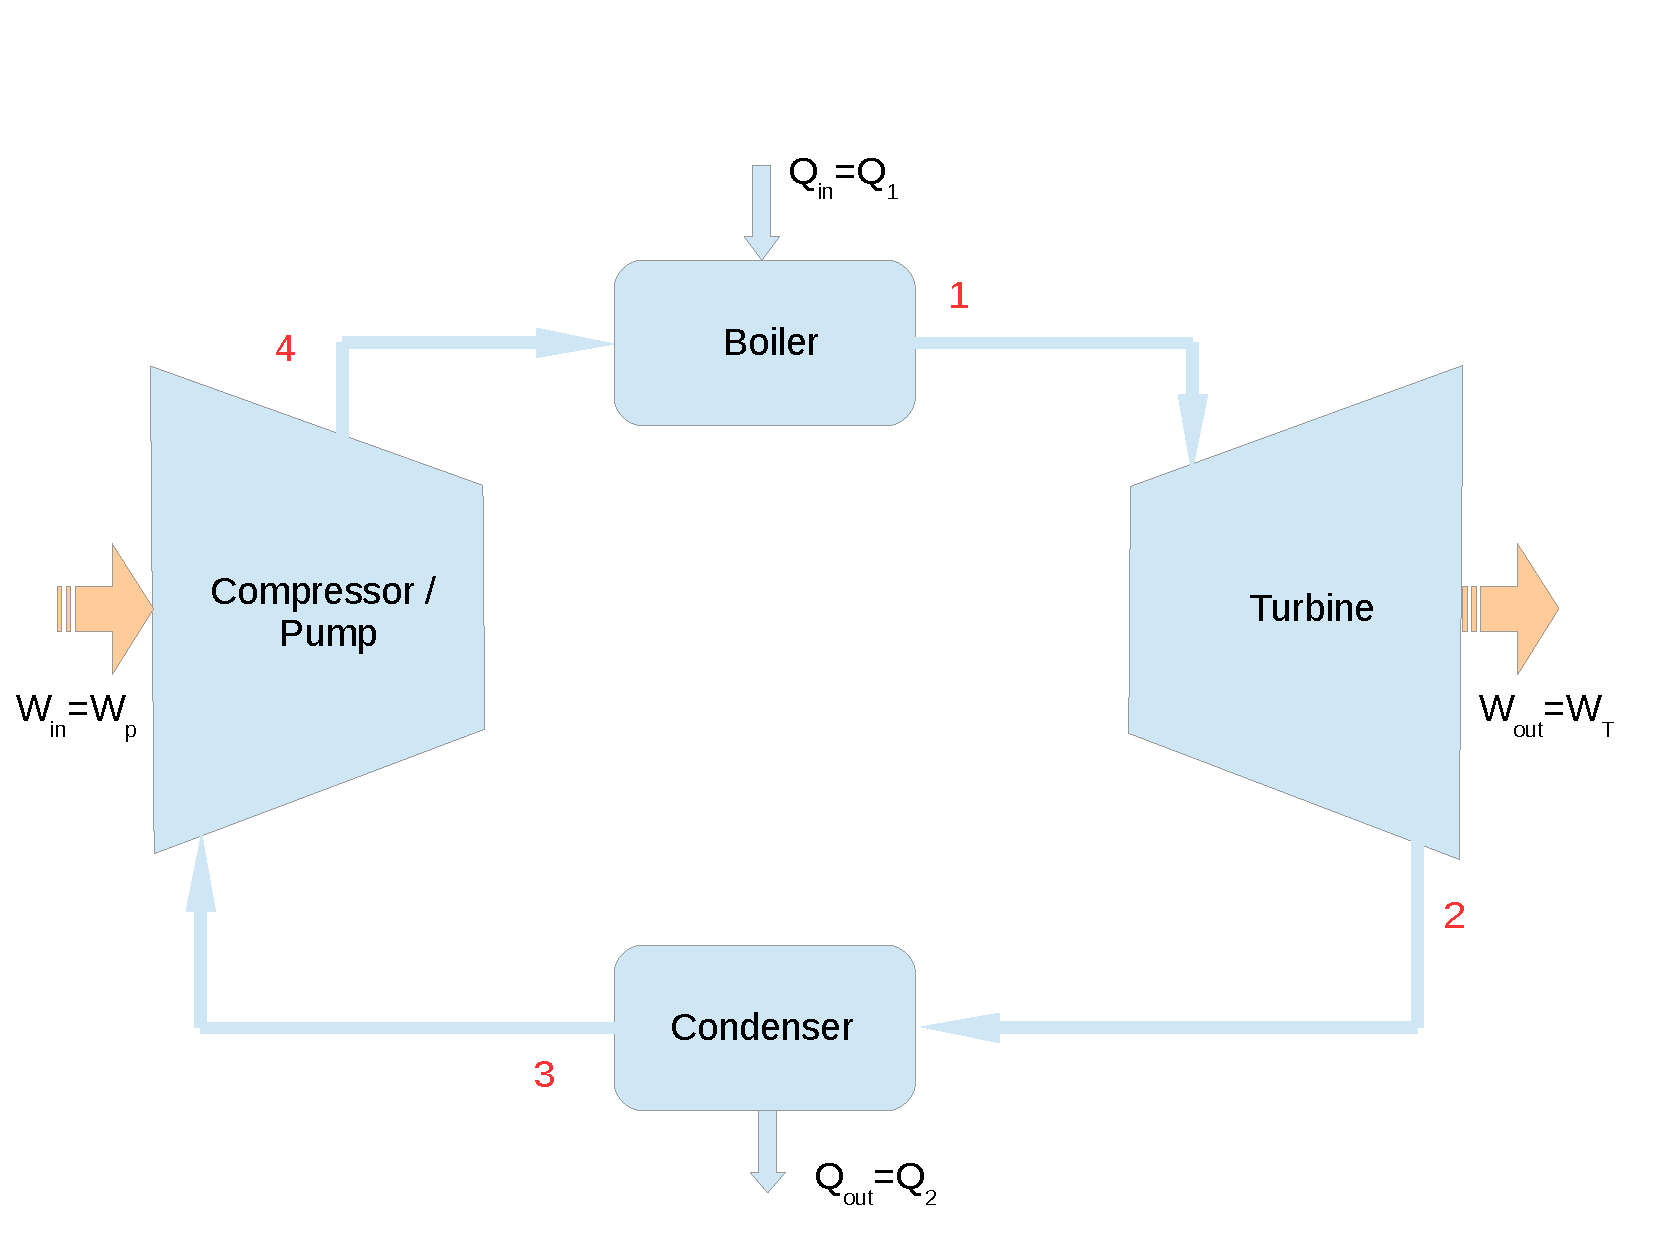
\includegraphics[width=\columnwidth,clip]{./Pics/Fig_SteamPowerPlant2}
           \caption{{\it Schematics of a simplified steam power plant.}} 
        \end{center}
      \end{figure}
    \end{column}
  \end{columns}
\end{frame}

%%%
%%% Slide
%%%
\subsection{Bibliography} 
\begin{frame}
 \frametitle{Suggested References}
  Literature relevant for this module:
  \begin{enumerate}[(a)]
   \item J.M. Smith, H.C. Van Ness, M.M. Abbott, $\lq$Introduction to Chemical Engineering Thermodynamics', 6$^{th}$ Edition: Chapters 2.1-5, 2.8-11, 5-6;
   \item A.B. Pippard, $\lq$Elements of Classical Thermodynamics' (1966): Chapters 2, 3 and 4;
   \item H. Devoe, $\lq$Thermodynamics and Chemistry', 2$^{nd}$ Edition: Chapters 2.5-6, 3.1-5,9,10 and 4;
   \item M.J. Moran, H.N. Saphiro, D.D. Boettner, M.B. Bailey, $\lq$Principles of Engineering Thermodynamics', 7$^{th}$ Edition: Chapters 1.2-8, 2, 3.1-8, 5 and 6.
  \end{enumerate}
\end{frame}

%%%
%%% Slide
%%%
\subsection{An {\it Extremely Short History} of Thermodynamics}
\begin{frame}
 \frametitle{Introduction}

   \begin{block}{1650s: $\lq$Birth' of the scientific discipline:}
   \textcolor{blue}{Boyle and Hooke found the classic relationship between pressure, temperature and volume.}
   \end{block}


   \begin{block}{1854: Scottish physicist William Thomson (Lord Kelvin)}
     \begin{itemize}
       \item \textcolor{blue}{$\lq$Thermo-dynamics is the subject of the relation of heat to forces acting between contiguous parts of bodies, and the relation of heat to electrical agency.'}
       \item \textcolor{blue}{Kelvin scale temperature (1848)}
       \item \textcolor{blue}{$\lq$Joule-Thompson effect' in gas liquefaction (1852)}
     \end{itemize}
   \end{block}

   \begin{block}{1871: Scottish mathematical physicist James Clerk Maxwell}
     \begin{itemize}
       \item \textcolor{blue}{1856-1869: Professor at Marischal College.}
       \item \textcolor{blue}{Maxwell's Laws of Eletromagnestism (1861-1881).}
       \item \textcolor{blue}{Kinetic theory -- Maxwell-Boltzmann distribution (1860-1866).}
       \item \textcolor{blue}{Maxwell's Thermodynamic relations (1871).}
     \end{itemize}
   \end{block}

\end{frame}

%%%
%%% SECTION
%%%
\section{Definitions}

\subsection{The Thermodynamic System}
%%%
%%% Slide
%%%
\begin{frame}
 \frametitle{Introduction}
  \begin{enumerate}[(a)]
   \item <2-> Thermodynamics is the study of energy and its transformations;
   \item <3-> It deals with overall energy and entropy changes, and their relation to direction of reactions and the position of equilibrium;
   \item <4-> Thermodynamics embodies a macroscopic viewpoint, i.e., it focuses on properties of a system (e.g., temperature, volume and heat capacity);
   \item <5-> Thermodynamics can be applied to systems in equilibrium and non-equilibrium;
   \item <6-> In this course we focus on system on equilibrium thermodynamics relevant to engineering problems.   
  \end{enumerate}
\end{frame}


%%%
%%% Slide
%%%
\begin{frame}
 \frametitle{General Remarks}
  \begin{enumerate}[(a)]
   \item <1-> Thermodynamics {\bf does}
     \begin{itemize}
       \item<2-> describe a system macroscopically;
       \item<2-> calculate the $\lq$energy' required for a physical or chemical process;
       \item<2-> determine a system's equilibrium conditions;
     \end{itemize}
   \item<3-> Thermodynamics {\bf does not}
     \begin{itemize}
       \item<4-> allow for kinetic considerations of chemical or physical processes;
       \item<4-> describe molecular behaviour.
     \end{itemize}
  \end{enumerate}
\end{frame}

%%%
%%% SUB-SECTION
%%%
\subsection{Dimensions and Units}

%%%
%%% Slide
%%%
\begin{frame}
 \frametitle{General Remarks}
  \begin{enumerate}[(a)]
   \item <1-> Do always use \textcolor{blue}{SI units} for calculations:
     \begin{itemize}
       \item<1-> second (s), meter (m), gram (g), Kelvin (K), mole (mol);
     \end{itemize}
   \item<2-> Or those based on them:
     \begin{itemize}
       \item<4-> Newton (N), Joule (J), Pascal (Pa).
     \end{itemize}
  \end{enumerate}

  \begin{center}
    \begin{tabular}{c c c | c c c}
      \hline
      {\it Multiple} & {\it Prefix} & {\it Symbol} & {\it Multiple} & {\it Prefix} & {\it Symbol} \\
      \hline
      10$^{-15}$      & femto        & f            &   10$^{2}$     &  hecto       & h            \\
      10$^{-12}$      & pico         & p            &   10$^{3}$     &  kilo        & k            \\
      10$^{-9}$       & nano         & n            &   10$^{6}$     &  mega        & M            \\
      10$^{-6}$       & micro        & $\mu$        &   10$^{9}$     &  giga        & G            \\
      10$^{-3}$       & milli        & m            &   10$^{12}$    &  tera        & T            \\
      10$^{-2}$       & centi        & c            &   10$^{15}$    &  peta        & P            \\
      \hline
    \end{tabular}
  \end{center}
\end{frame}


%%%
%%% Slide
%%%
\begin{frame}
 \frametitle{Summary}
  \begin{enumerate}[(a)]
   \item <1-> Measures of amount or size:
     \begin{itemize}
       \item<1-> Mass ($m$), number of moles ($n$), total volume $\left(V^{t}\right)$;
       \item<1-> Specific volume $\left(V=V^{t}/m\right)$;
     \end{itemize}
   \item<1-> Force ($F$), pressure ($P$), temperature ($T$);
   \item<1-> Work ($W$), heat ($Q$);
   \item<1-> Energy ($E$)potential and kinetic.
  \end{enumerate} 
\end{frame}

%%%
%%% Slide
%%%
\begin{frame}
 \frametitle{Unit Conversion}
  \begin{enumerate}[(a)]
   \item<1-> Most of the time, we need to convert units during our calculations. Thus if we want to convert pressure ($P$) from {\it atm} to {\it psi} (pounds per square inch):
      \begin{displaymath}
        P = 5\;\cancel{\text{atm}} \times \textcolor{red}{\displaystyle\frac{14.70\;\text{psi}}{1\;\cancel{\text{atm}}}} = 73.50\;psi
      \end{displaymath}
   \item<2-> Or, in a more complex example -- $dH=VdP$:
      \begin{eqnarray}
        H_{2} &=& H_{1} + V_{1}\left(P_{2}-P_{1}\right) \nonumber \\
              &=& 706.9\textcolor{red}{\frac{kJ}{kg}} + 1.1111\times 10^{-3}\textcolor{blue}{\frac{m^{3}}{kg}}\left(210.0-7.4\right)\textcolor{blue}{bar} \nonumber \\
              &=& 706.9\textcolor{red}{\frac{kJ}{kg}} + 1.1111\times 10^{-3}\textcolor{blue}{\frac{\cancel{m^{3}}}{\cancel{kg}}} 202.6\;\textcolor{blue}{\cancel{bar}} \textcolor{red}{\frac{10^{5}\;\frac{\cancel{kg}}{\cancel{m}.\cancel{s^{2}}}}{1\; \cancel{bar}}} \textcolor{red}{\frac{10^{-3}\; \frac{kJ}{kg}}{1\;\frac{\cancel{m^{2}}}{\cancel{s^{2}}}}} \nonumber \\
              &=& 729.41\textcolor{red}{\frac{kJ}{kg}} \nonumber 
      \end{eqnarray} 
  \end{enumerate}
\end{frame}


%%%
%%% SUB-SECTION
%%%
\subsection{Overall System Analysis}

%%%
%%% Slide
%%%
\scriptsize
\begin{frame}
 \frametitle{System and Control Volumes}
  \begin{columns}
    \begin{column}[l]{0.6\linewidth}
      \begin{itemize}%\scriptsize
       \item <2-> The thermodynamic system is the part of the universe we are considering. We are free to choose boundary conditions.
       \item <3-> A \textcolor{red}{system} is defined as a quantity of matter or a region in space chosen for study;
       \item <4-> The mass or region outside the system is called the \textcolor{red}{surroundings};
       \item <5-> The real or imaginary surface that separates the system from its surroundings is called the \textcolor{red}{boundary};
       \item <6-> Systems may be considered to be {\it closed} or {\it open}, depending on whether a fixed mass or a fixed volume in space is chosen for study; 
      \end{itemize}
    \end{column}
    \begin{column}[l]{0.4\linewidth}\scriptsize
      \begin{figure}%
        \begin{center}
          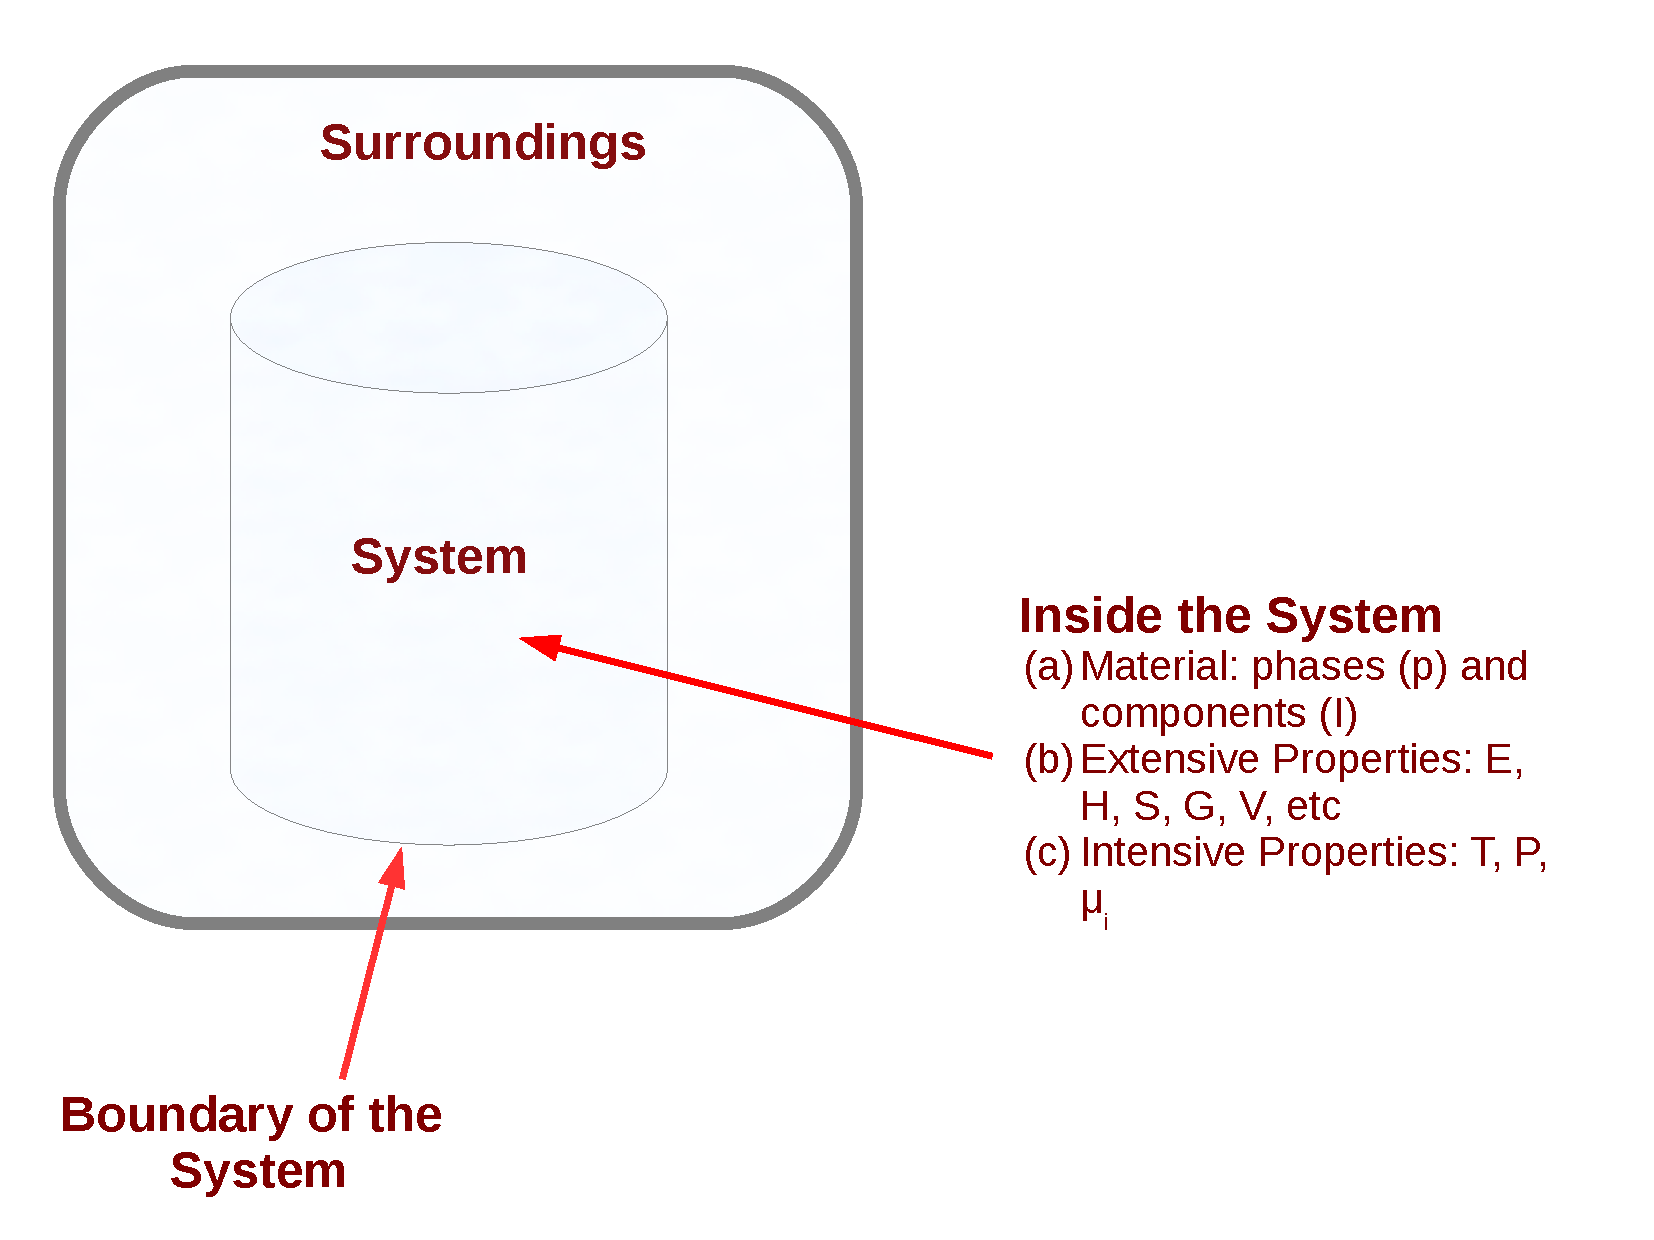
\includegraphics[width=\columnwidth,clip]{./Pics/Fig_SystemDefinition}
        \end{center}
      \end{figure}
      \begin{tabular}{|c|c|c|}
         \hline
                      & {\bf Mass} & {\bf Energy} \\
                      & {\bf Exchange} & {\bf Exchange} \\
         \hline
         {\bf Open}   & {\it yes}  & {\it yes}    \\
         {\bf Closed} & {\it no}   & {\it yes}    \\
         {\bf Isolated}&{\it no}   & {\it no}     \\
         \hline 
      \end{tabular}    
    \end{column}
  \end{columns}
\end{frame}
\normalsize



%%%
%%% Slide
%%%
\scriptsize
\begin{frame}
 \frametitle{System and Control Volumes}
  \begin{columns}
    \begin{column}[l]{0.6\linewidth}
      \begin{itemize}%\scriptsize
       \item <1-> A \textcolor{red}{closed system} (also known as a \textcolor{red}{control mass}) consists of a fixed amount of mass, and no mass can cross its boundary. However, energy (in the form of heat or work) may cross the boundary -- and the volume of a closed system does not have to be fixed; 
       \item <2-> When neither energy nor mass is allowed to cross the boundary, that system is called an \textcolor{red}{isolated system};
       \item <3-> An open system (or \textcolor{red}{control volume}) is a properly selected region in space. It usually encloses a device that involves mass flow such as a compressor, turbine, or nozzle.
      \end{itemize}
    \end{column}
    \begin{column}[l]{0.4\linewidth}\scriptsize
      \begin{figure}%
        \begin{center}
          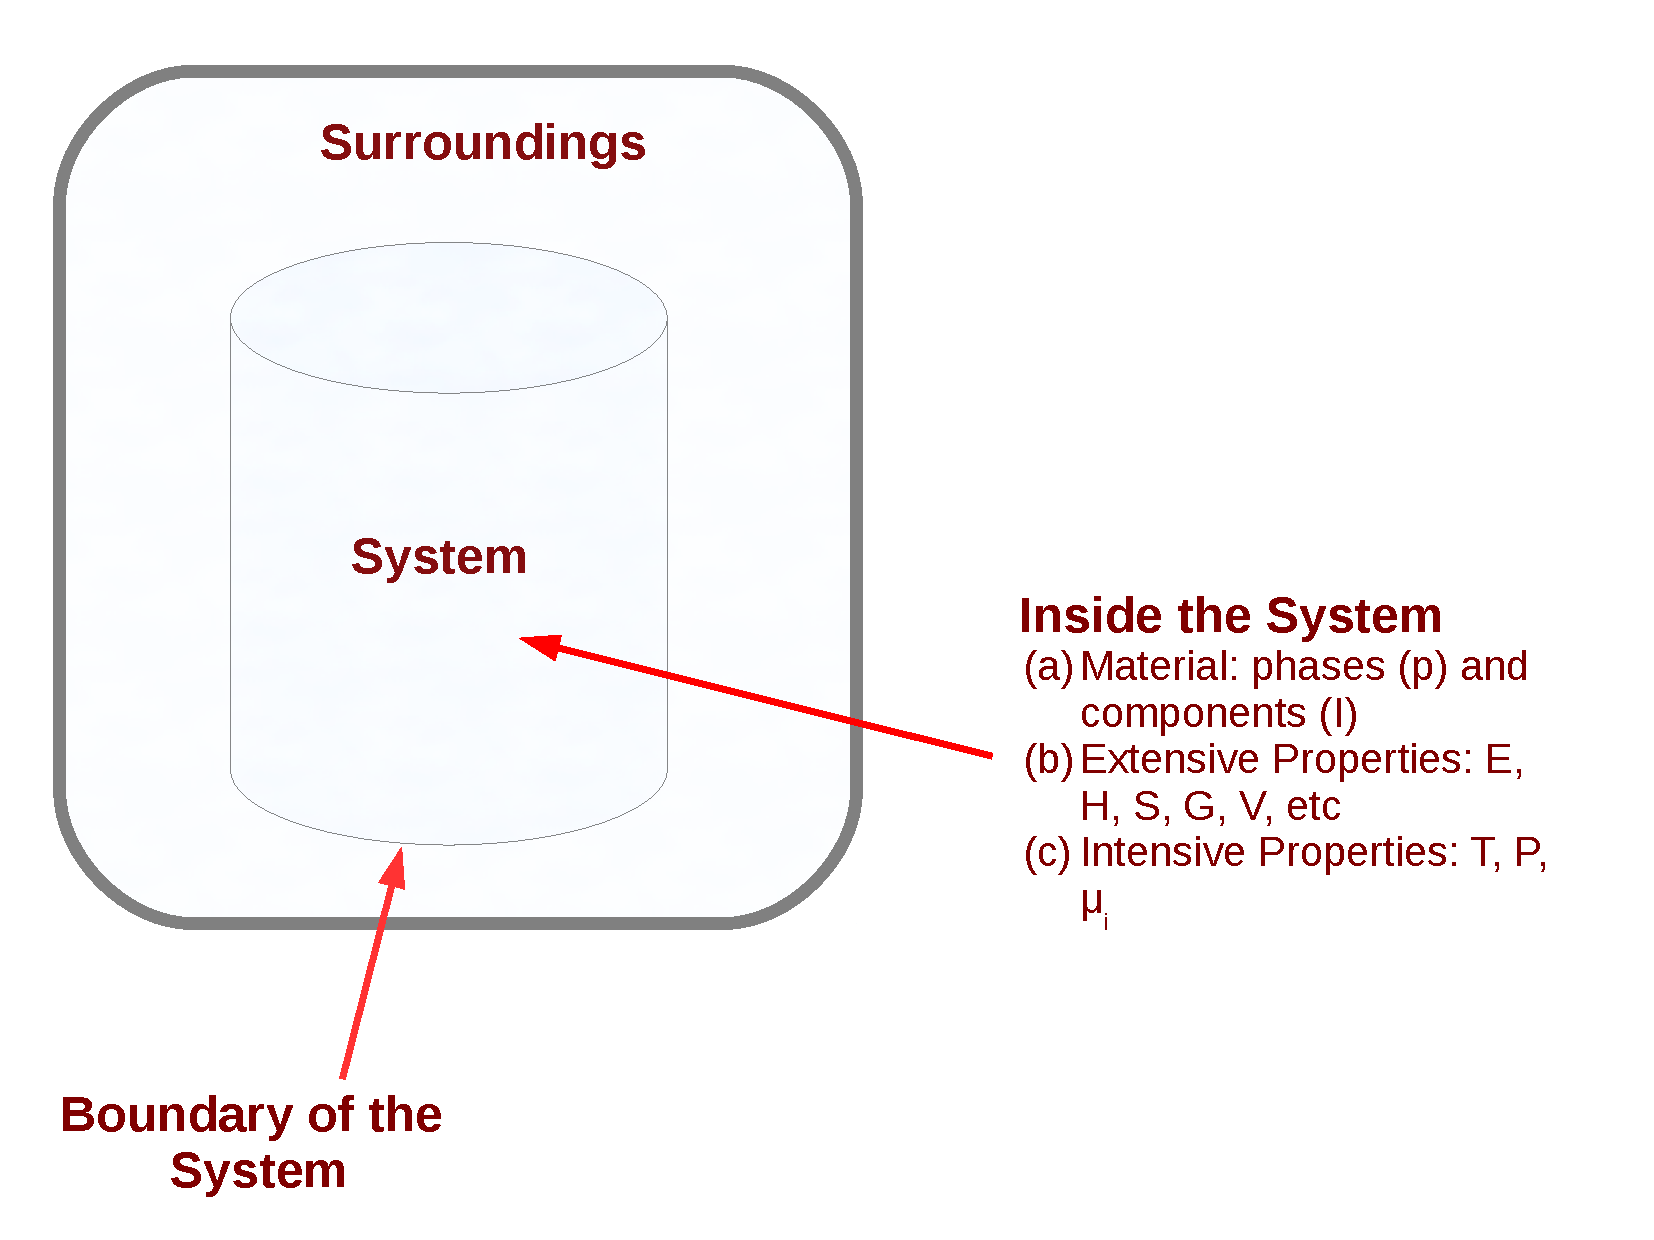
\includegraphics[width=\columnwidth,clip]{./Pics/Fig_SystemDefinition}
        \end{center}
      \end{figure}
      \begin{tabular}{|c|c|c|}
         \hline
                      & {\bf Mass} & {\bf Energy} \\
                      & {\bf Exchange} & {\bf Exchange} \\
         \hline
         {\bf Open}   & {\it yes}  & {\it yes}    \\
         {\bf Closed} & {\it no}   & {\it yes}    \\
         {\bf Isolated}&{\it no}   & {\it no}     \\
         \hline 
      \end{tabular}    
    \end{column}
  \end{columns}
\end{frame}
\normalsize


%%%
%%% Slide
%%%
\begin{frame}
 \frametitle{System and Control Volumes}
 \begin{itemize}
  \item <2-> The \textcolor{red}{material} in a system is composed of phases (e.g., solid, liquid, gas) with distinct physical and chemical properties;
  \item <3-> The \textcolor{red}{composition} of each phase is described by a series of discrete chemical formula units (i.e., chemical components) -- e.g., water/steam $\left(\right.$H$_{2}$O$\left.\right)$, ammonia $\left(\right.$NH$_{3}\left.\right)$, carbon dioxide $\left(\right.$CO$_{2}\left.\right)$, etc;
  \item <4-> Any characteristic of a system is called a \textcolor{red}{property} -- e.g., pressure, temperature, mass, etc;
  \item <5-> Properties can be classified as \textcolor{red}{intensive} or \textcolor{red}{extensive};
  \item <6-> \textcolor{red}{Intensive properties} are those that are {\bf independent} of the mass of a system -- e.g., temperature, pressure, density, viscosity, etc;
  \item <7-> \textcolor{red}{Extensive properties} are those whose values {\bf depend} on the size (or extent) of the system -- e.g., mass, volume, number of moles, internal energy, enthalpy, entropy, etc.  
 \end{itemize}
\end{frame}



%%%
%%% SECTION
%%%
\section{Review of the Main Tools for the Course}

\subsection{PVT Surfaces}
%%%
%%% Slide
%%%

\begin{frame}
 \frametitle{PVT Behaviour of Pure Substances}
 \begin{columns}
  \begin{column}[l]{0.5\linewidth}
\begin{itemize}
\item <1-> This surface represents the \textcolor{red}{Pressure} - \textcolor{red}{specific volume} - \textcolor{red}{Temperature} -- $PVT$, relation in a pure substance;
\item <2-> Any given coordinate in both, the surface plot and diagrams (projections), will represent values of pressure, specific volume and temperature when the substance is at equilibrium;
\end{itemize}
  \end{column}
  \begin{column}[l]{0.5\linewidth}
   \begin{figure}%
    \begin{center}
     \includegraphics[width=4.cm,clip]{./Pics/PVT_Surface.jpg}
    \end{center}
\caption{$PVT$ surface (top) and projections onto (b) $PT$ and (c) $PV$ diagrams for a pure substance (Extracted from Moran {\it et al.})}
   \end{figure}    
  \end{column}
 \end{columns}
\end{frame}



%%%
%%% Slide
%%%

\begin{frame}
 \frametitle{PVT Behaviour of Pure Substances}
 \begin{columns}
  \begin{column}[l]{0.5\linewidth}
\begin{itemize}
\item <1-> The \textcolor{red}{Gibbs phase rule},
\begin{equation}
\Psi = 2 + \mathcal{C} - \mathcal{P}
\end{equation} 
\item <2-> describes the number of degrees of freedom (dof), $\Psi$ (intensive variables, e.g., temperature, pressure), in a closed system at equilibrium as a function of the number of phases ($\mathcal{P}$ = solid, liquid and vapour) and components, $\mathcal{C}$ (e.g., water, CO$_{2}$, N$_{2}$, etc). 
\end{itemize}
  \end{column}
  \begin{column}[l]{0.5\linewidth}
   \begin{figure}%
    \begin{center}
     \includegraphics[width=4.cm,clip]{./Pics/PVT_Surface.jpg}
    \end{center}
\caption{$PVT$ surface (top) and projections onto (b) $PT$ and (c) $PV$ diagrams for a pure substance (Extracted from Moran {\it et al.})}
   \end{figure}    
  \end{column}
 \end{columns}
\end{frame}


%%%
%%% Slide
%%%

\begin{frame}
 \frametitle{PVT Behaviour of Pure Substances}
 \begin{columns}
  \begin{column}[l]{0.5\linewidth}
\begin{itemize}
\item <1-> {\bf Example:} In the $PT$ diagram (b) for one hypothetical component -- $\textcolor{red}{\mathcal{C}=1}$, within each phase region -- $\textcolor{blue}{\mathcal{P}=1}$ (i.e., as either solid, liquid or vapour phases),
\begin{displaymath}
\Psi = 2 + \textcolor{red}{1} - \textcolor{blue}{1} = 2
\end{displaymath}
\item <2-> In this case, the number of degrees of freedom correspond to temperature and pressure;
\item <3-> Thus, within (e.g.) the vapour phase, temperature and pressure can readily be changed without explicit phase change or composition of the vapour phase.
\end{itemize}
  \end{column}
  \begin{column}[l]{0.5\linewidth}
   \begin{figure}%
    \begin{center}
     \includegraphics[width=4.cm,clip]{./Pics/PVT_Surface.jpg}
    \end{center}
\caption{$PVT$ surface (top) and projections onto (b) $PT$ and (c) $PV$ diagrams for a pure substance (Extracted from Moran {\it et al.})}
   \end{figure}    
  \end{column}
 \end{columns}
\end{frame}


%%%
%%% Slide
%%%

\begin{frame}
 \frametitle{PVT Behaviour of Pure Substances}
 \begin{columns}
  \begin{column}[l]{0.5\linewidth}
\begin{itemize}
\item <1-> However, along with the \textcolor{red}{phase-line boundary}, two phases are in equilibrium, i.e., $\textcolor{blue}{\mathcal{P}=2}$,%
\begin{displaymath}
\Psi = 2 + \textcolor{red}{1} - \textcolor{blue}{2} = 1
\end{displaymath}
\item <2-> When the vapour and liquid phases are in equilibrium, any change in temperature {\bf leads} to change in pressure for the system remains in equilibrium;
\end{itemize}
  \end{column}
  \begin{column}[l]{0.5\linewidth}
   \begin{figure}%
    \begin{center}
     \includegraphics[width=4.cm,clip]{./Pics/PVT_Surface.jpg}
    \end{center}
\caption{$PVT$ surface (top) and projections onto (b) $PT$ and (c) $PV$ diagrams for a pure substance (Extracted from Moran {\it et al.})}
   \end{figure}    
  \end{column}
 \end{columns}
\end{frame}


%%%
%%% Slide
%%%

\begin{frame}
 \frametitle{PVT Behaviour of Pure Substances}
 \begin{columns}
  \begin{column}[l]{0.5\linewidth}
\begin{itemize}
\item <1-> Similarly, for the {\bf triple point} -- $\textcolor{blue}{\mathcal{P}=3}$, all three phases are in equilibrium
\begin{displaymath}
\Psi = 2 + \textcolor{red}{1} - \textcolor{blue}{3} = 0
\end{displaymath}
\item <2-> Here there is {\bf no degrees of freedom} -- i.e., there is {\bf just} one value for pressure and temperature that make the {\bf three phases to coexist}.
\item <3-> Any change in either intensive properties will drive the system away from the {\it triple point}.
\end{itemize}
  \end{column}
  \begin{column}[l]{0.5\linewidth}
   \begin{figure}%
    \begin{center}
     \includegraphics[width=4.cm,clip]{./Pics/PVT_Surface.jpg}
    \end{center}
\caption{$PVT$ surface (top) and projections onto (b) $PT$ and (c) $PV$ diagrams for a pure substance (Extracted from Moran {\it et al.})}
   \end{figure}    
  \end{column}
 \end{columns}
\end{frame}

%%%
%%% SUBSECTION
%%%
\subsection{Thermodynamic Diagrams and Tables}

%%%
%%% Slide
%%%
\begin{frame}
 \frametitle{Thermodynamics Diagrams: $PH$ and $TS$}
   \begin{figure}%
     \vbox{
      \hbox{\hspace{.8cm}
      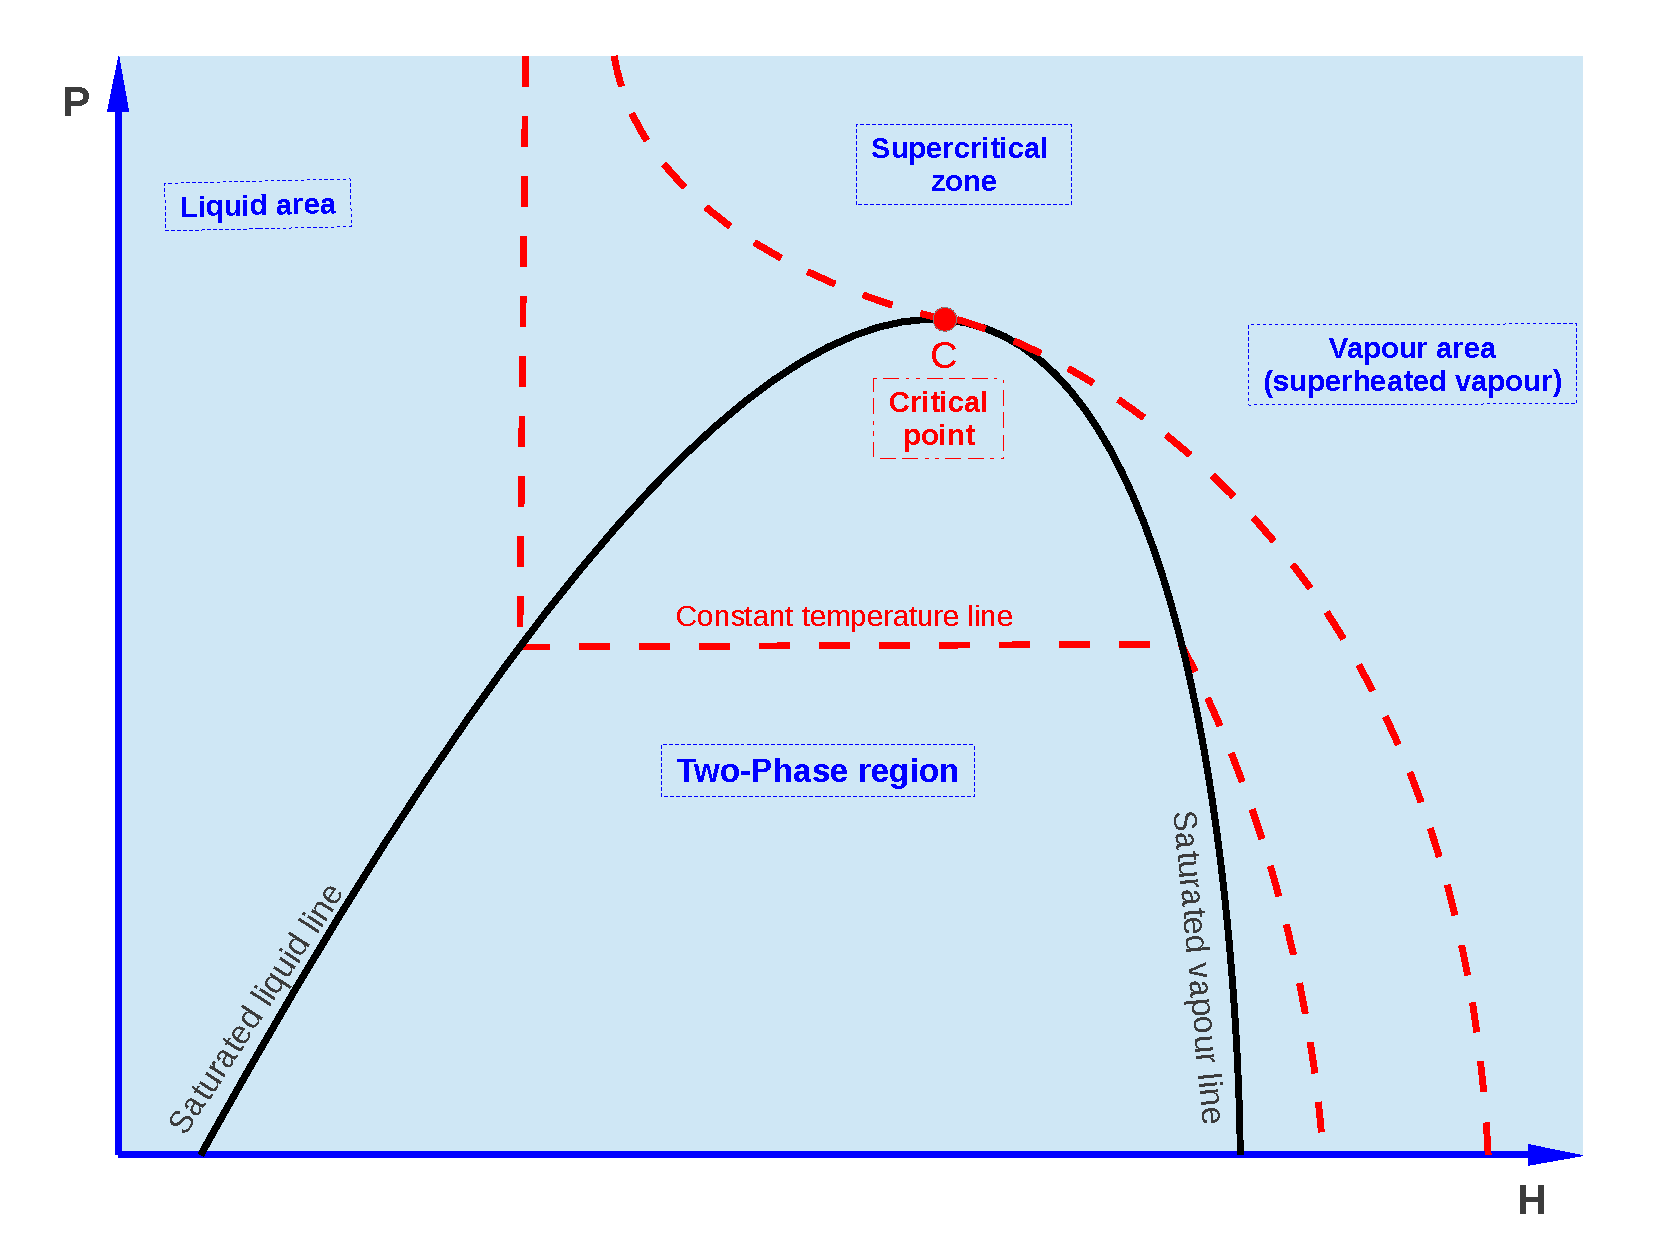
\includegraphics[width=4.6cm,height=3.8cm,clip]{./Pics/Overview_Refrig18}
      \hspace{.1cm}
      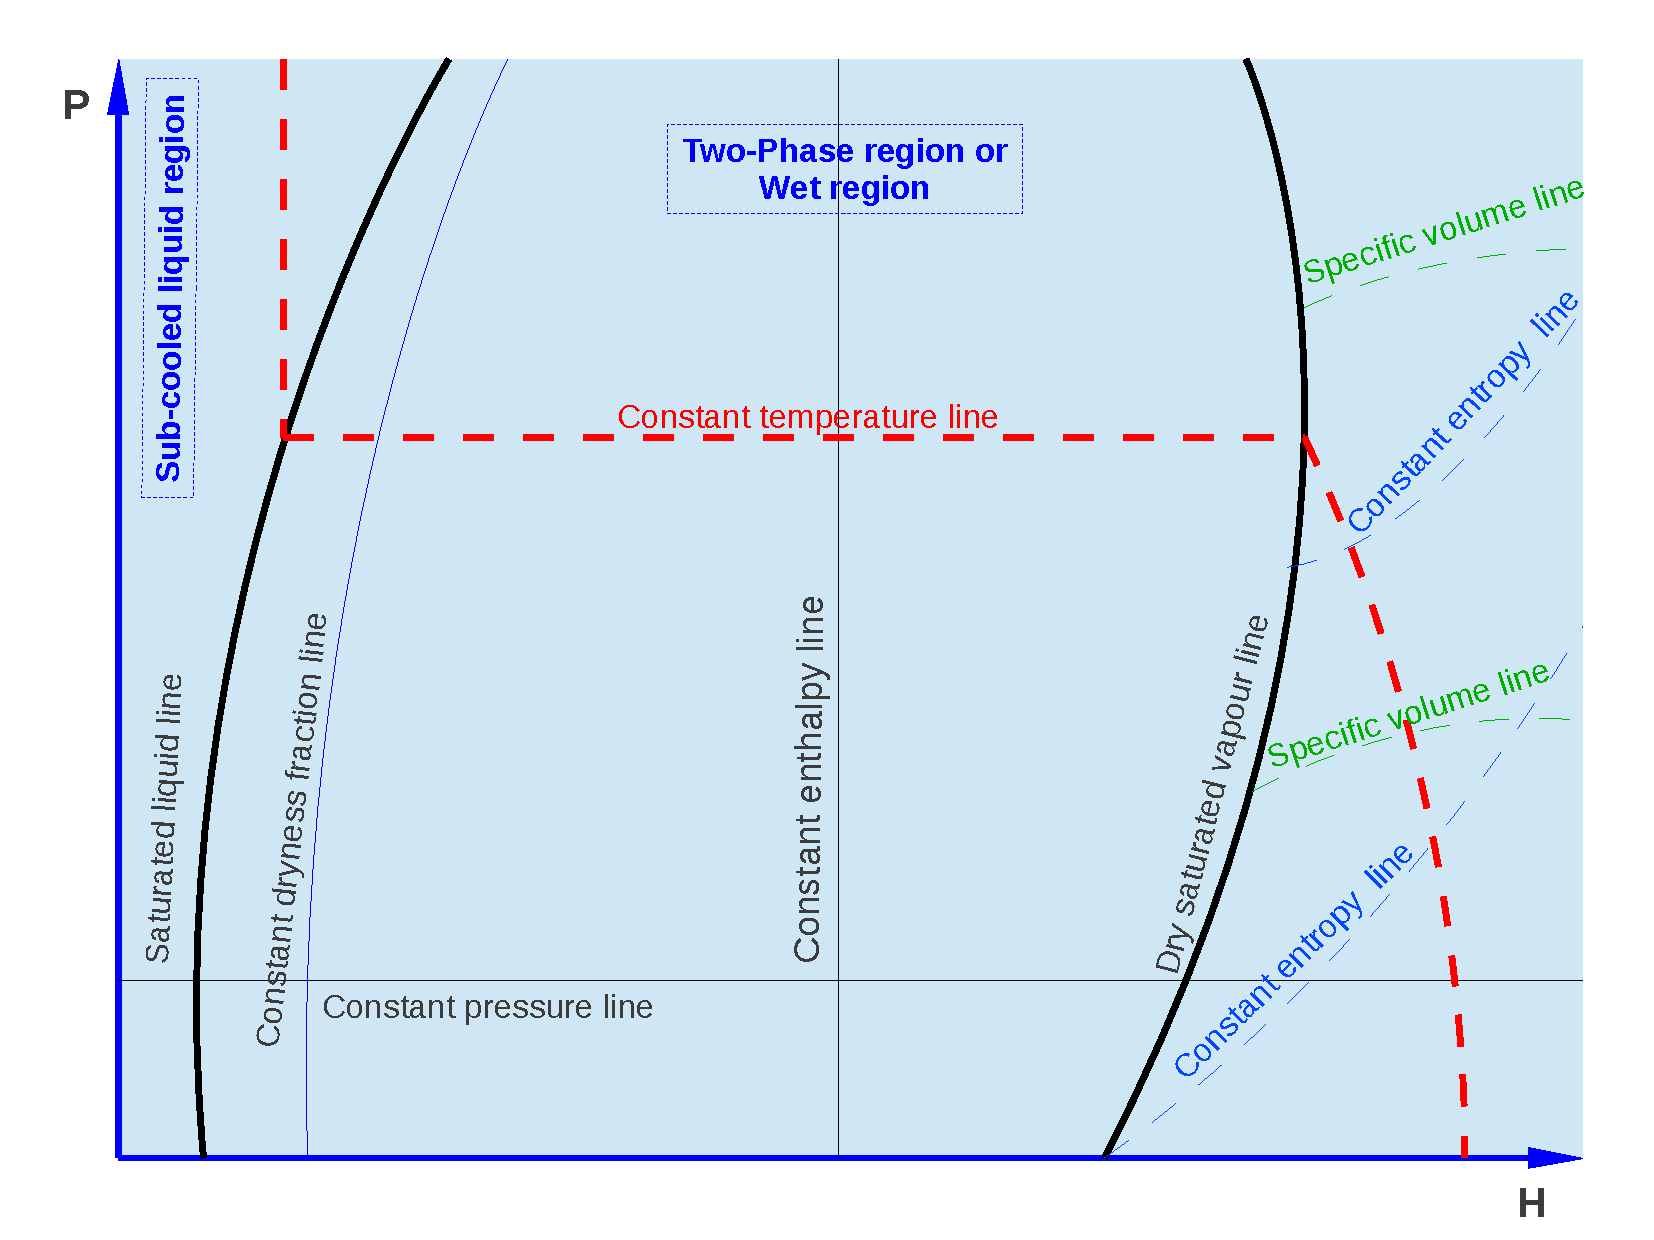
\includegraphics[width=4.6cm,height=3.8cm,clip]{./Pics/Overview_Refrig17}}
      \vspace{-.1cm}
      \hbox{\hspace{.8cm}
      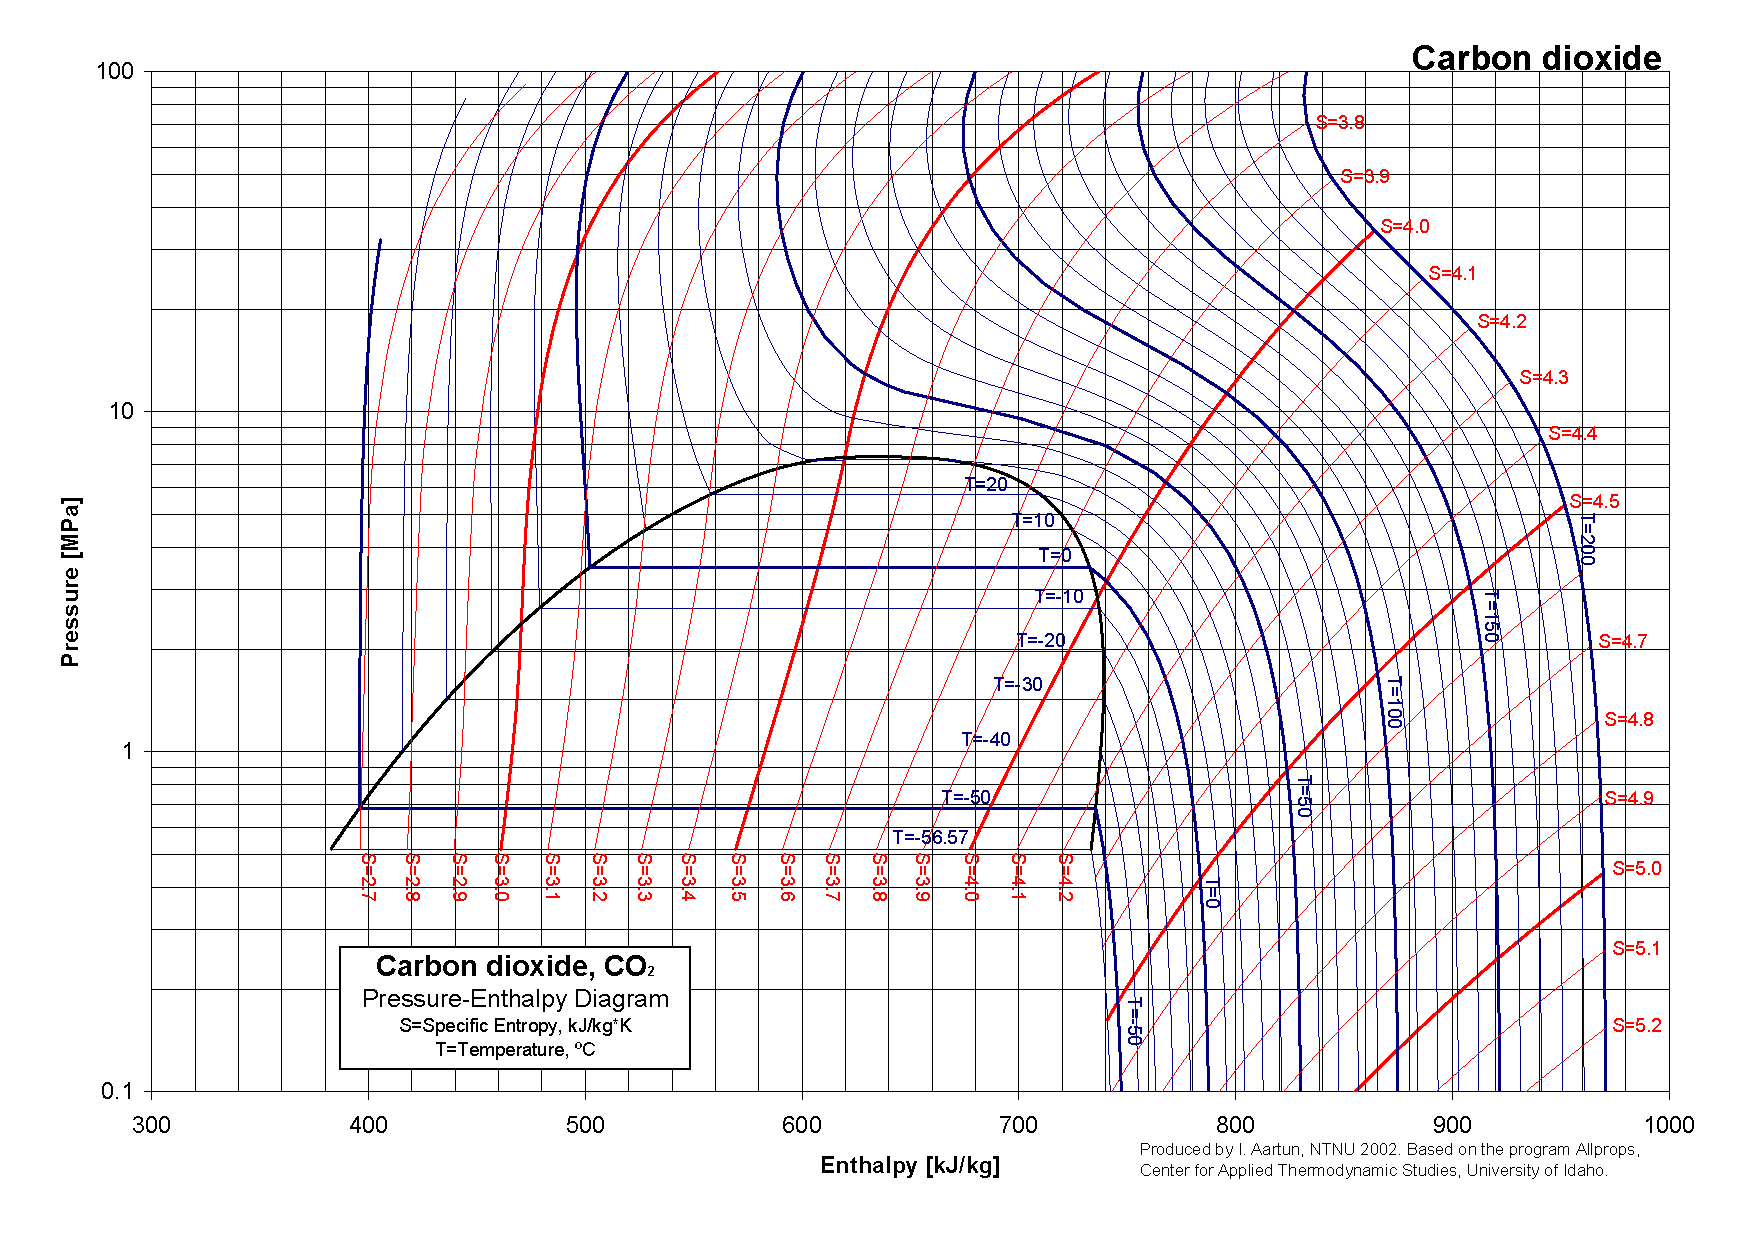
\includegraphics[width=4.9cm,height=4.cm,clip]{./Pics/CO2col}
      \hspace{.1cm}
      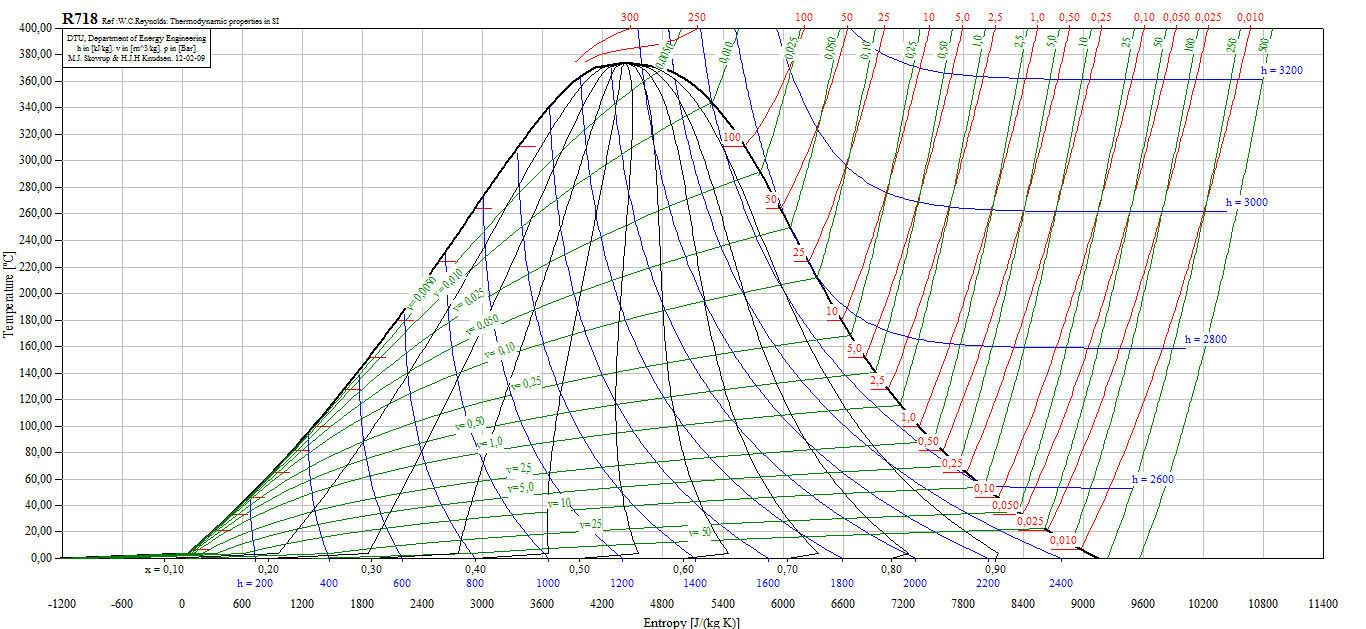
\includegraphics[width=4.6cm,height=3.87cm,clip]{./Pics/water_TS.png}}}
   \end{figure}
\end{frame}


%%%
%%% Slide
%%%

\begin{frame}
  \frametitle{Another option: Saturated and Superheated Steam Tables}
   \begin{figure}%
   \vbox{
      \hbox{\hspace{-1.cm}
      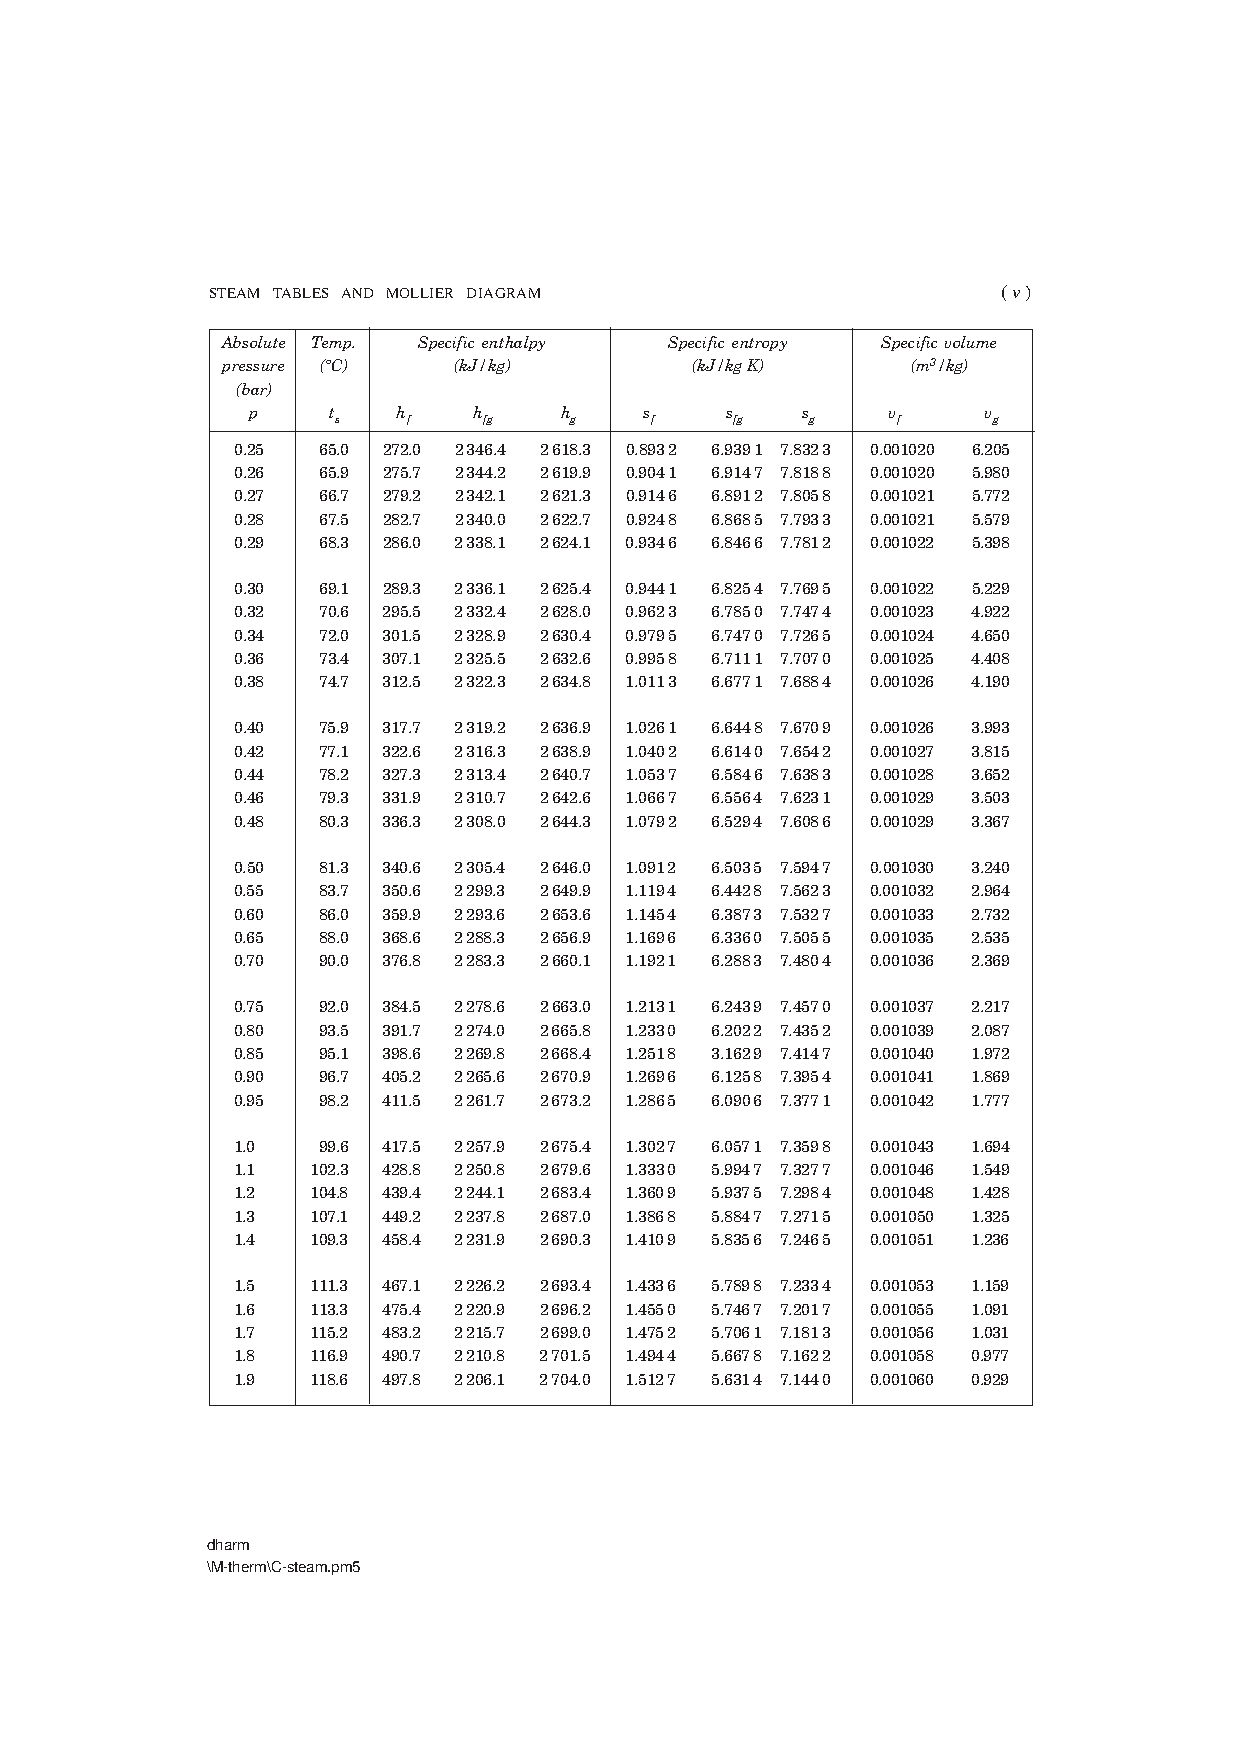
\includegraphics[width=8.cm,height=8.5cm,clip]{./Pics/Sample_SteamTablePg}
      \hspace{-2cm}
      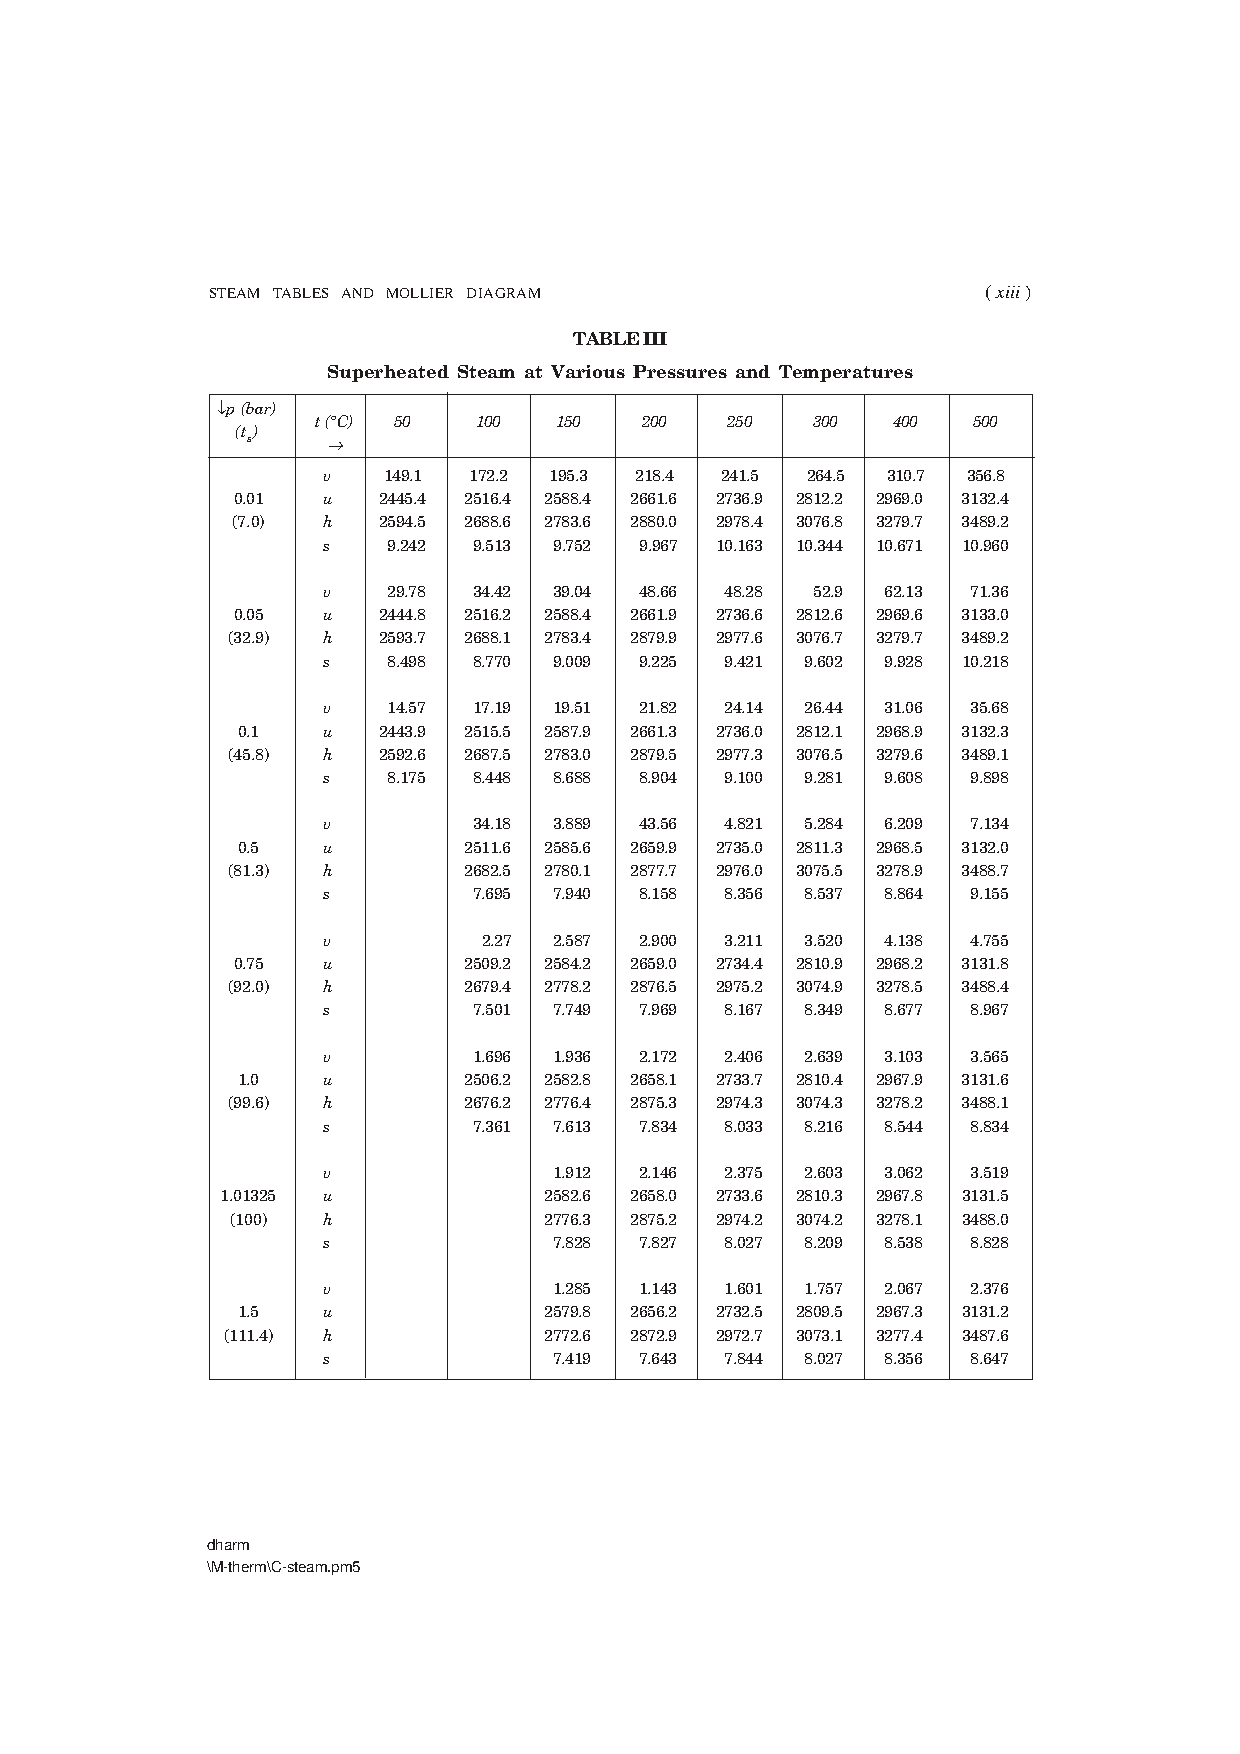
\includegraphics[width=8.cm,height=8.5cm,clip]{./Pics/Sample_SteamTablePg2}}}
   \end{figure}
\end{frame}


%%%
%%% Slide
%%%
\begin{frame}
  \frametitle{Another option: Saturated and Superheated Steam Tables}
\noindent
\begin{itemize}
\item <2-> {\bf \textcolor{red}{Example:}} At $P=1.50\;$ bar, the saturated steam has the following thermodynamic properties,
\tiny
\begin{center}
%\begin{table}[h]
\begin{tabular}{||c|c|c c c|c c c|c c||} 
\hline\hline
$P$ & $T$ & $H_{f}$ &  $H_{fg}$ & $H_{g}$ & $S_{f}$ &  $S_{fg}$ &  $S_{g}$ & $V_{f}$ & $V_{g}$ \\ 
\hline
1.50 & 111.3 & 467.1 & 2226.2 & 2693.4 & 1.4336 & 5.7898 & 7.2334 & 0.001053 & 1.159 \\
\hline
\end{tabular}
%\caption{Carnot and Rankine Cycles: From Saturated water and steam tables.}
%\label{Example01_01:Table2}
%\end{table}
\end{center}

\item <3-> But the properties of superheated steam at the same pressure will depend on the temperature $\Rightarrow$ \textcolor{red}{see superheated steam table}.

\item <2-> {\bf Units:} [$P$] = bar, [$T$] = $^{o}$C, [$H$]= $\frac{kJ}{kg}$, [$S$]=$\frac{kJ}{kg.K}$, [$V$]=$\frac{m^{3}}{kg}$.

\end{itemize}

\end{frame}

%%%
%%% SUBSECTION
%%%
\subsection{Linear Interpolation}
%%%
%%% Slide
%%%
\begin{frame}
  \frametitle{Linear Interpolation}
\noindent
\begin{itemize}
\item <2-> Some of the problems in this course involves extracting values from the thermodynamic tables;
\item <3-> And although the tables are very extensive (for most of the materials), sometimes we need values that can not be directly found on them;
\item <4-> In this case, we just operate a {\bf linear interpolation} between neighbour fields;
\item <5-> For example, water-steam at 1.5 bar and 212$^{o}$C;
\item <6-> At this pressure, the {\bf saturation temperature} is 111.3$^{o}$C, therefore we know that the fluid (water/steam) is at \textcolor{red}{superheated state};
\end{itemize}

\end{frame}

%%%
%%% Slide
%%%

\begin{frame}
  \frametitle{Linear Interpolation}
\noindent
\begin{itemize}
\item <2-> Thus at 1.5 bar, the enthalpies at 200 and 250$^{o}$C are $H_{1}=2872.9\frac{kJ}{kg}$ and $H_{2}=2972.7\frac{kJ}{kg}$, respectively.
\item <3-> The enthalpy at 212$^{o}$C,
\begin{tabular}{ l l }
\scriptsize $\Delta T=T_{2}-T_{1}=250-200^{o}$C   & \scriptsize $\longleftrightarrow$  $\Delta H=H_{2}-H_{1}=2972.7-2872.9=99.8\frac{kJ}{kg}$ \\
\scriptsize $\Delta T^{\star} = T_{2} - T^{\star}= 250 - 212^{\circ}$C & \scriptsize $\longleftrightarrow$  $\Delta H^{\star}= H_{2} - H^{\star}= 2972.7 - H^{\star}$\\    
\end{tabular}
\item <4-> $\Delta H^{\star}=75.848\frac{kJ}{kg}$ 
\item <5-> Thus $\Delta H^{\star}= H_{2}-H^{\star} \longrightarrow H^{\star}=2896.85\frac{kJ}{kg}$
\end{itemize}

\end{frame}


%%%
%%% SECTION
%%%
\section{Laws of Thermodynamics}

\subsection{Zeroth Law of Thermodynamics}

%%%
%%% Slide
%%%
\begin{frame}
 \frametitle{Zeroth Law of Thermodynamics (Thermal Equilibrium)}

 \begin{columns}
  \begin{column}[r]{0.4\linewidth}
   \begin{block}{R.H. Fowler (1931)}
   \textcolor{blue}{$\lq$Two bodies are in equilibrium if both have the same temperature reading even if they are not in contact.'}
   \end{block}
    $ T_{j} = T_{i}
    \begin{cases}
     \forall_{i}, \forall{j} \\
     i \neq j
    \end{cases}$
  \end{column}
  
  \begin{column}[c]{0.6\linewidth}
\scriptsize \textcolor{blue}{Two bodies reaching thermal equilibrium after being brought into contact in an isolated enclosure.}
   \begin{figure}%
    \begin{center}
     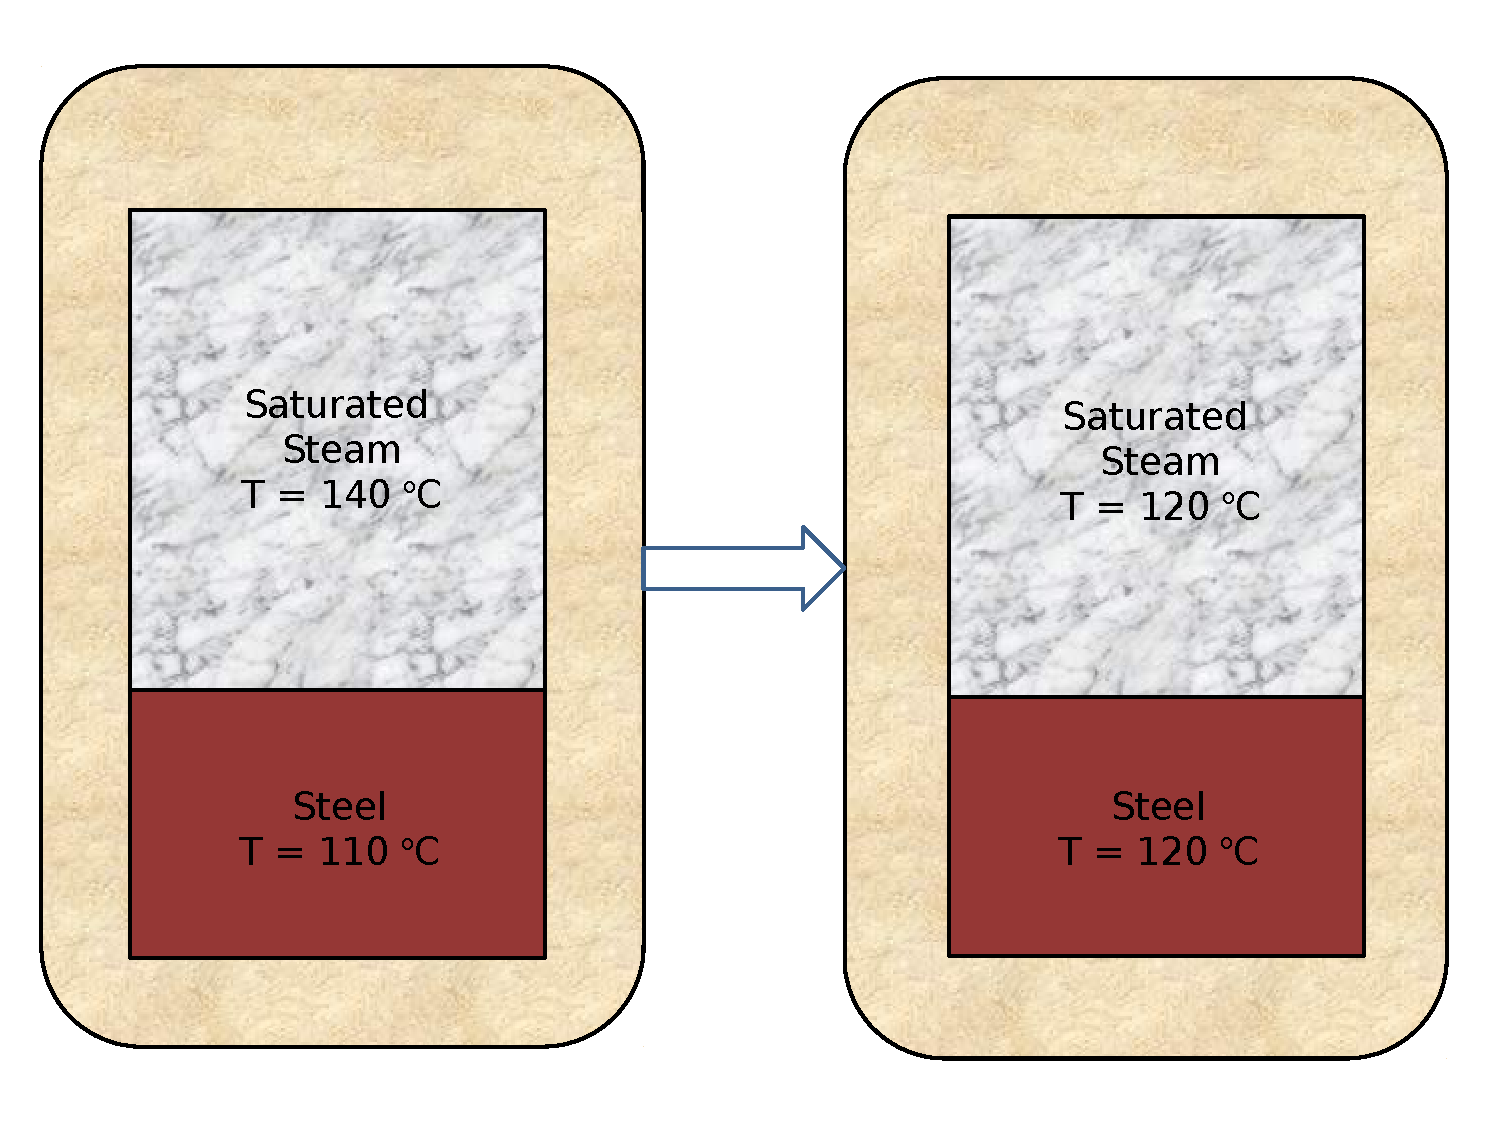
\includegraphics[width=\columnwidth,clip]{./Pics/zeroth_law}\\
      \scriptsize \textcolor{blue}{$t = 0 \hspace{3.cm} \text{equilibrium state}$}
    \end{center}
   \end{figure}
  \end{column}
 \end{columns}

\end{frame}

%%%
%%% SUBSECTION
%%%
\subsection{First Law of Thermodynamics}

%%%
%%% Slide
%%%
\begin{frame}
 \frametitle{First Law of Thermodynamics (Conservation of Work)}
 %\scriptsize

 \begin{block}{R. Clausius and J.P. Joule (1850)}
  \textcolor{blue}{$\lq$For all adiabatic processes between two specified states of a closed system, the net work done is the same regardless of the nature of the closed system and the details of the process.}
  \begin{center}
   \textcolor{red}{or}
  \end{center}
  \textcolor{blue}{$\lq$Although energy assumes many forms, the total quantity of energy is constant, and when energy disappears in one form it appears simultaneously in other forms.}'
 \end{block}


 \begin{itemize}
  \item<2-> It states that energy can neither be created, nor can it be destroyed. This means that the total amount of energy in the universe always remains conserved;
  \item<3-> Energy can be changed from one form to another. There are many different forms of energy, some of which may be more useful than others for a particular process;
 \end{itemize}

\normalsize
\end{frame}

%%%
%%% Slide
%%%
\begin{frame}
 \frametitle{First Law of Thermodynamics (Conservation of Energy)}
 %\scriptsize
   \begin{enumerate}
      \item<1-> A system (e.g., a fluid) can possess energy:
        \begin{itemize}
          \item<1-> as a result of its macroscopic position (potential) or movement (kinetic);
          \item<1-> or as a result of microscopic/molecular motion $\rightarrow$ {\it internal energy}.
        \end{itemize}
\visible<2->{
      \begin{block}{Conservation of Energy}
        \begin{center}
          \textcolor{blue}{$\Delta E$ (system) + $\Delta E$ (surroundings) = 0}
        \end{center}
      \end{block}}

      \item<3-> Heat and work represent energy in transint across boundaries -- system and surroundings.

   \end{enumerate}
\normalsize
\end{frame}

%%%
%%% Slide
%%%
\begin{frame}
 \frametitle{First Law of Thermodynamics (Conservation of Energy in Closed Systems)}
 %\scriptsize
   \begin{enumerate} 
      \item<1-> Closed systems $\longrightarrow$ $dm = 0$
         \visible<1->{
         \begin{center}
           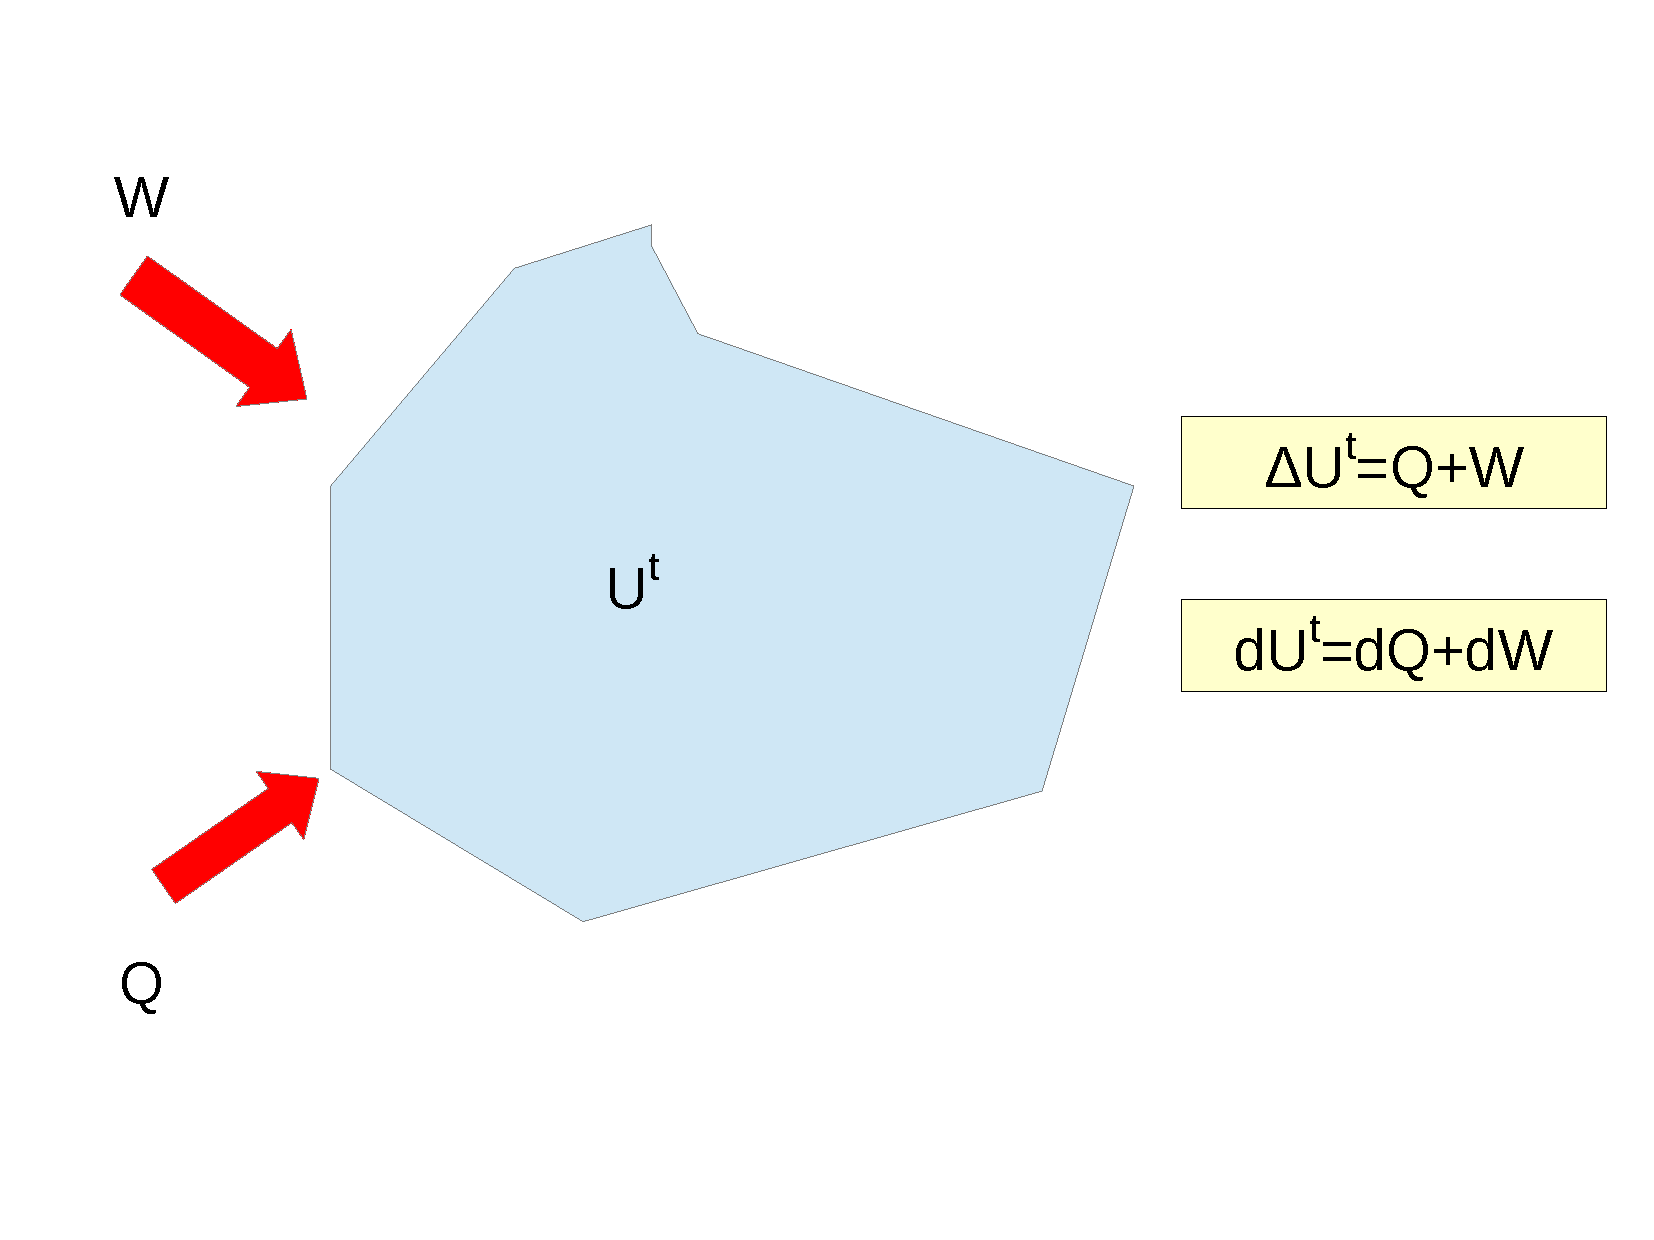
\includegraphics[width=6.cm,clip]{./Pics/Energy_ClosedSystems}
         \end{center}}
      \item<2-> \href{http://www.iupac.org/}{IUPAC} (International Union of Pure and Applied Chemistry) sign convention:
         \begin{itemize}
            \item<2-> Heat ($Q$) and work ($W$)  always refer to the system;
            \item<2-> Energy transfer to the system has always a \textcolor{blue}{positive sign}.
         \end{itemize}
   \end{enumerate}
\normalsize
\end{frame}


%%%
%%% Slide
%%%
\begin{frame}
 \frametitle{Representations of the First Law -- Cycle}

 \begin{block}{}During any cycle, the cyclic integral of heat added to a system is proportional to the cyclic integral of work done by the system.\end{block}

 The mathematical representation of the first law is
 \begin{equation}
  \displaystyle\oint \delta Q = \displaystyle\oint \delta W
  \label{Module00:first_law}
 \end{equation}
 with {\it [Q] = J} and {\it [W] = J}.

\end{frame}

%%%
%%% Slide
%%%
\begin{frame}
 \frametitle{Representations of the First Law -- Cycle}
 %\scriptsize
 \begin{columns}
  \begin{column}[l]{0.5\linewidth}
   \begin{itemize}
    \item <1-> \textcolor{blue}{Power cycle}: systems (e.g., rhs) that deliver a net work transfer of energy to their surroundings during each cycle;
    \item <2-> $W_{cycle} = Q_{in} - Q_{out}$ with $Q_{in} > Q_{out}$ for a power cycle;
    \item <3-> The energy supplied by heat transfer to a system on a power cycle is normally derived from combustion (also from nuclear fission or solar radiation). The energy $Q_{out}$ is generally discharged to the surrounding atmosphere or a nearby body of water;
   \end{itemize}
  \end{column}
   
  \begin{column}[l]{0.5\linewidth}
   \begin{figure}%
    \begin{center}
     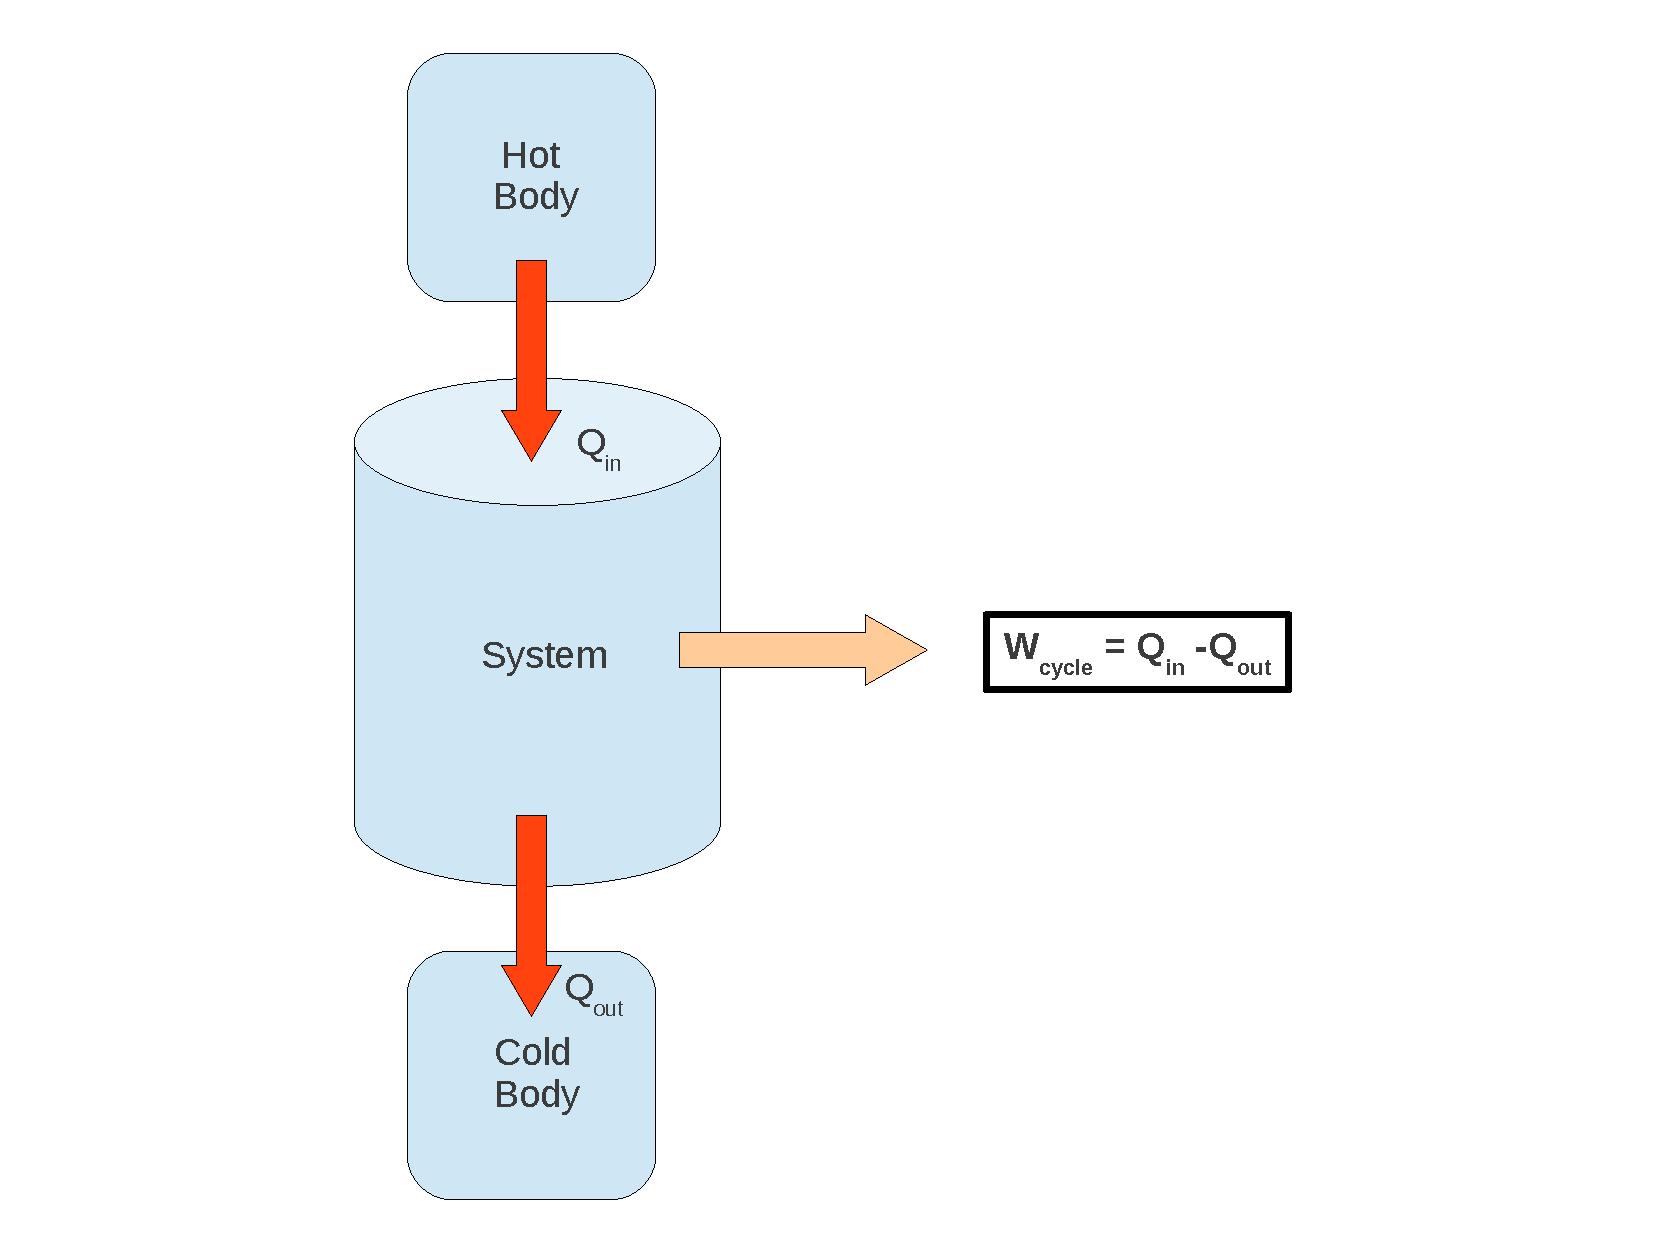
\includegraphics[width=8.cm,clip]{./Pics/FirstLaw_Cycle_01}
    \end{center}
   \end{figure}    
  \end{column}
 \end{columns}
 \normalsize
\end{frame}


%%%
%%% Slide
%%%
\begin{frame}
 \frametitle{Representations of the First Law -- Cycle}
 %\scriptsize
 \begin{columns}
  \begin{column}[l]{0.5\linewidth}
   \begin{itemize}
    \item <1-> \textcolor{blue}{Thermal efficiency}: $\eta =\displaystyle\frac{W_{cycle}}{Q_{in}} = \displaystyle\frac{Q_{in} - Q_{out}}{Q_{in}} = 1 - \displaystyle\frac{Q_{out}}{Q_{in}} < 1$;
    \item <2-> For reversible power cycles the ratio of heat transfer, $Q_{cold}/Q_{hot}$ depends only on the reservoir temperatures: $Q_{cold}/Q_{hot} = T_{cold}/T_{hot}$;
    \item <3-> Thus the thermal efficiency of a reversible power cycle while operating between thermal reservoirs at temperatures $T_{hot}$ and $T_{cold}$ is expressed as,\\
          $\eta_{max} = 1 - \displaystyle\frac{T_{cold}}{T_{hot}}$
   \end{itemize}
  \end{column}
   
  \begin{column}[l]{0.5\linewidth}
   \begin{itemize}
    \item <4-> This is the \textcolor{blue}{Carnot efficiency} and it is the maximum efficiency any power cycle can have while operating between the 2 reservoirs.
   \end{itemize}\vspace{-.5cm}
   \begin{figure}%
    \begin{center}
     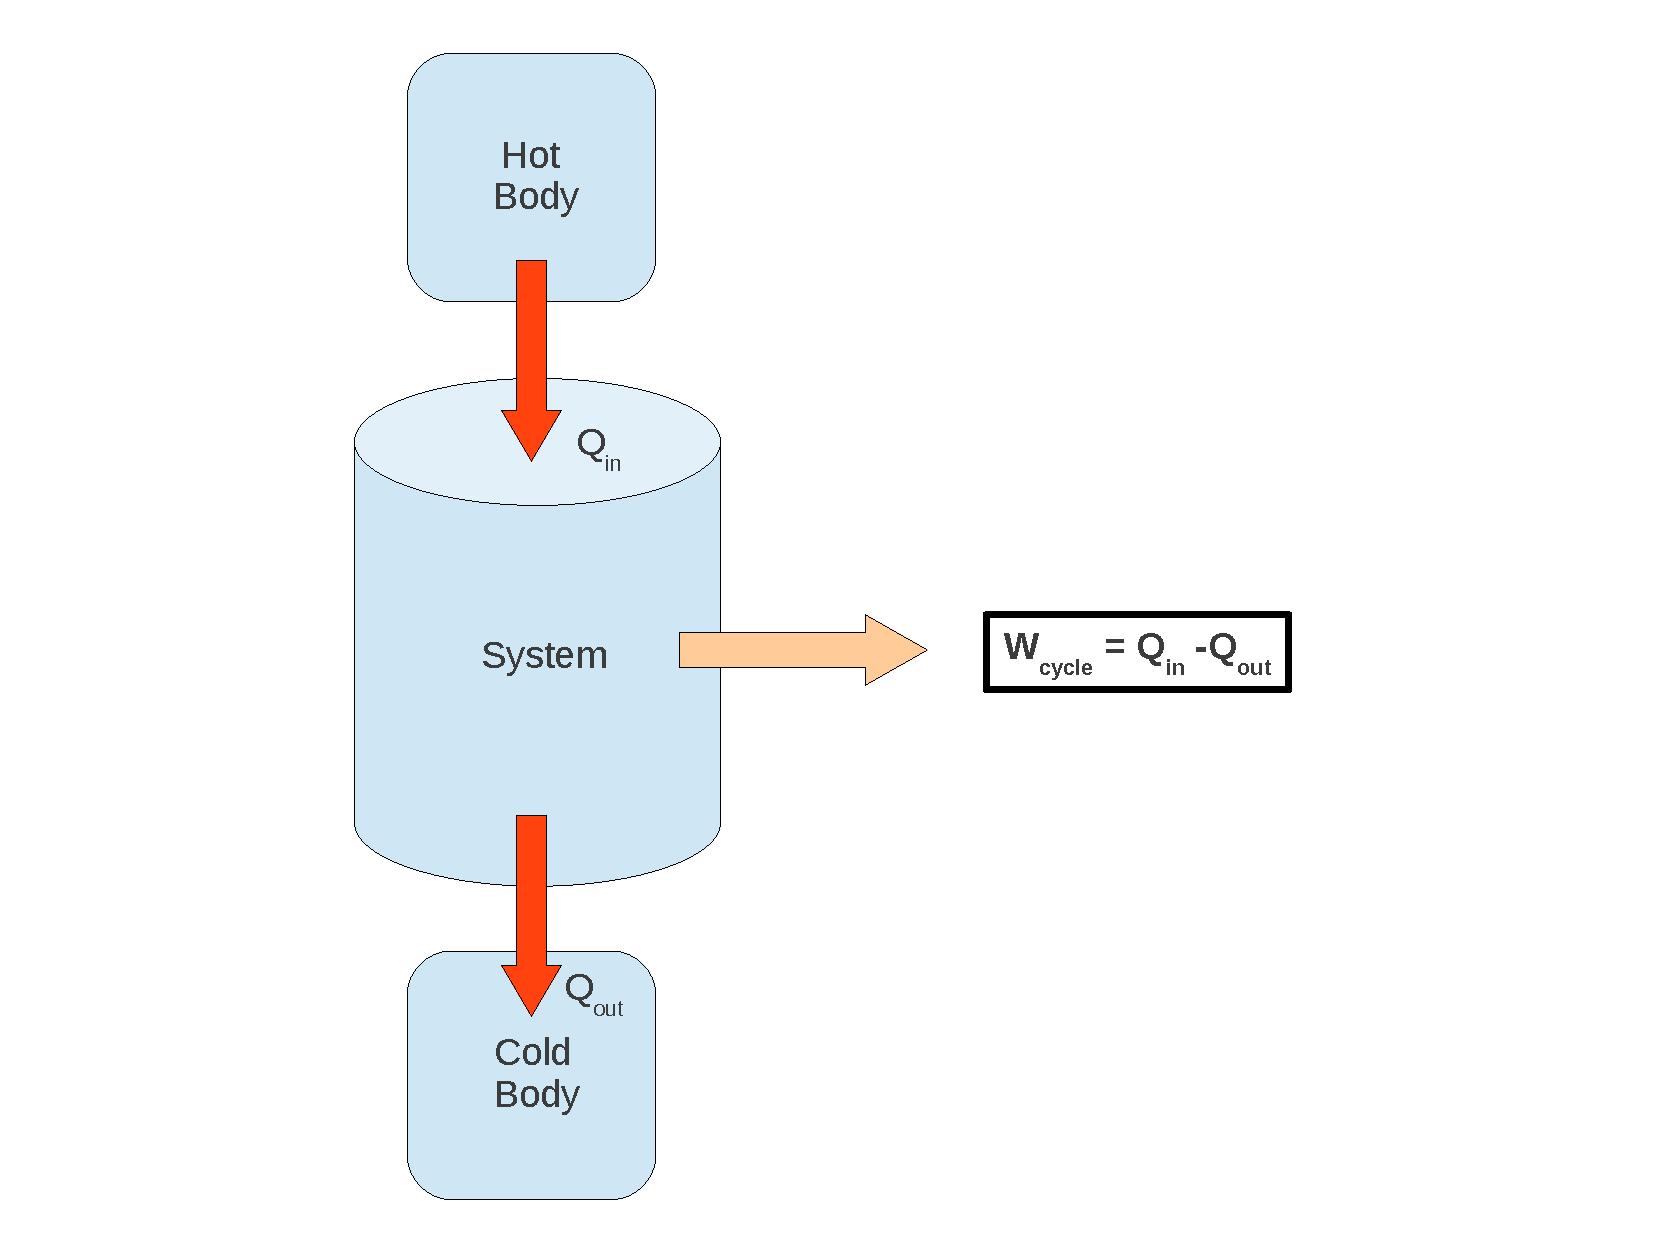
\includegraphics[width=8.cm,clip]{./Pics/FirstLaw_Cycle_01}
    \end{center}
   \end{figure}    
  \end{column}
 \end{columns}
 \normalsize
\end{frame}


%%%
%%% Slide
%%%
\begin{frame}
 \frametitle{Representations of the First Law -- Cycle}
 \begin{columns}
  \begin{column}[l]{0.5\linewidth}
   \begin{itemize}%\scriptsize
    \item <1-> \textcolor{blue}{Refrigerators} and \textcolor{blue}{Heat Pumps} Cycles (rhs): cycles in which Q$_{in}$ is associated with the heat energy transferred into the system from the cold body. Q$_{out}$ is the energy discharged via heat transfer from the system to the hot body;
    \item <2-> $W_{cycle} = Q_{out} - Q_{in}$% > 0 \Longrightarrow Q_{out} > Q_{in}$
    \item <3-> \textcolor{blue}{Refrigeration cycle}:
     \begin{enumerate}[(a)]%\scriptsize
      \item <4-> Objective: to cool a refrigerated body or to maintain the temperature of a body bellow that of the surroundings;
      \item <5-> Coefficient of Performance: $\beta = \displaystyle\frac{Q_{in}}{W_{cycle}} = \displaystyle\frac{Q_{in}}{Q_{out} - Q_{in}}$;
      %\item <6-> E.g., in a fridge: cavity contents $\xrightarrow{Q_{in}}$ refrigerant fluid $\left(T_{fluid} < T_{cavity}\right)$ $\xrightarrow{Q_{out}}$ surrounding air; 
     \end{enumerate}
    \end{itemize}
  \end{column}
   
  \begin{column}[c]{0.5\linewidth}
     \begin{enumerate}[(c)]%\scriptsize
      \item <6-> E.g., in a fridge: cavity contents $\xrightarrow{Q_{in}}$ refrigerant fluid $\left(T_{fluid} < T_{cavity}\right)$ $\xrightarrow{Q_{out}}$ surrounding air; 
     \end{enumerate}
\vspace{-.5cm}
   \begin{figure}%
    \begin{center}
     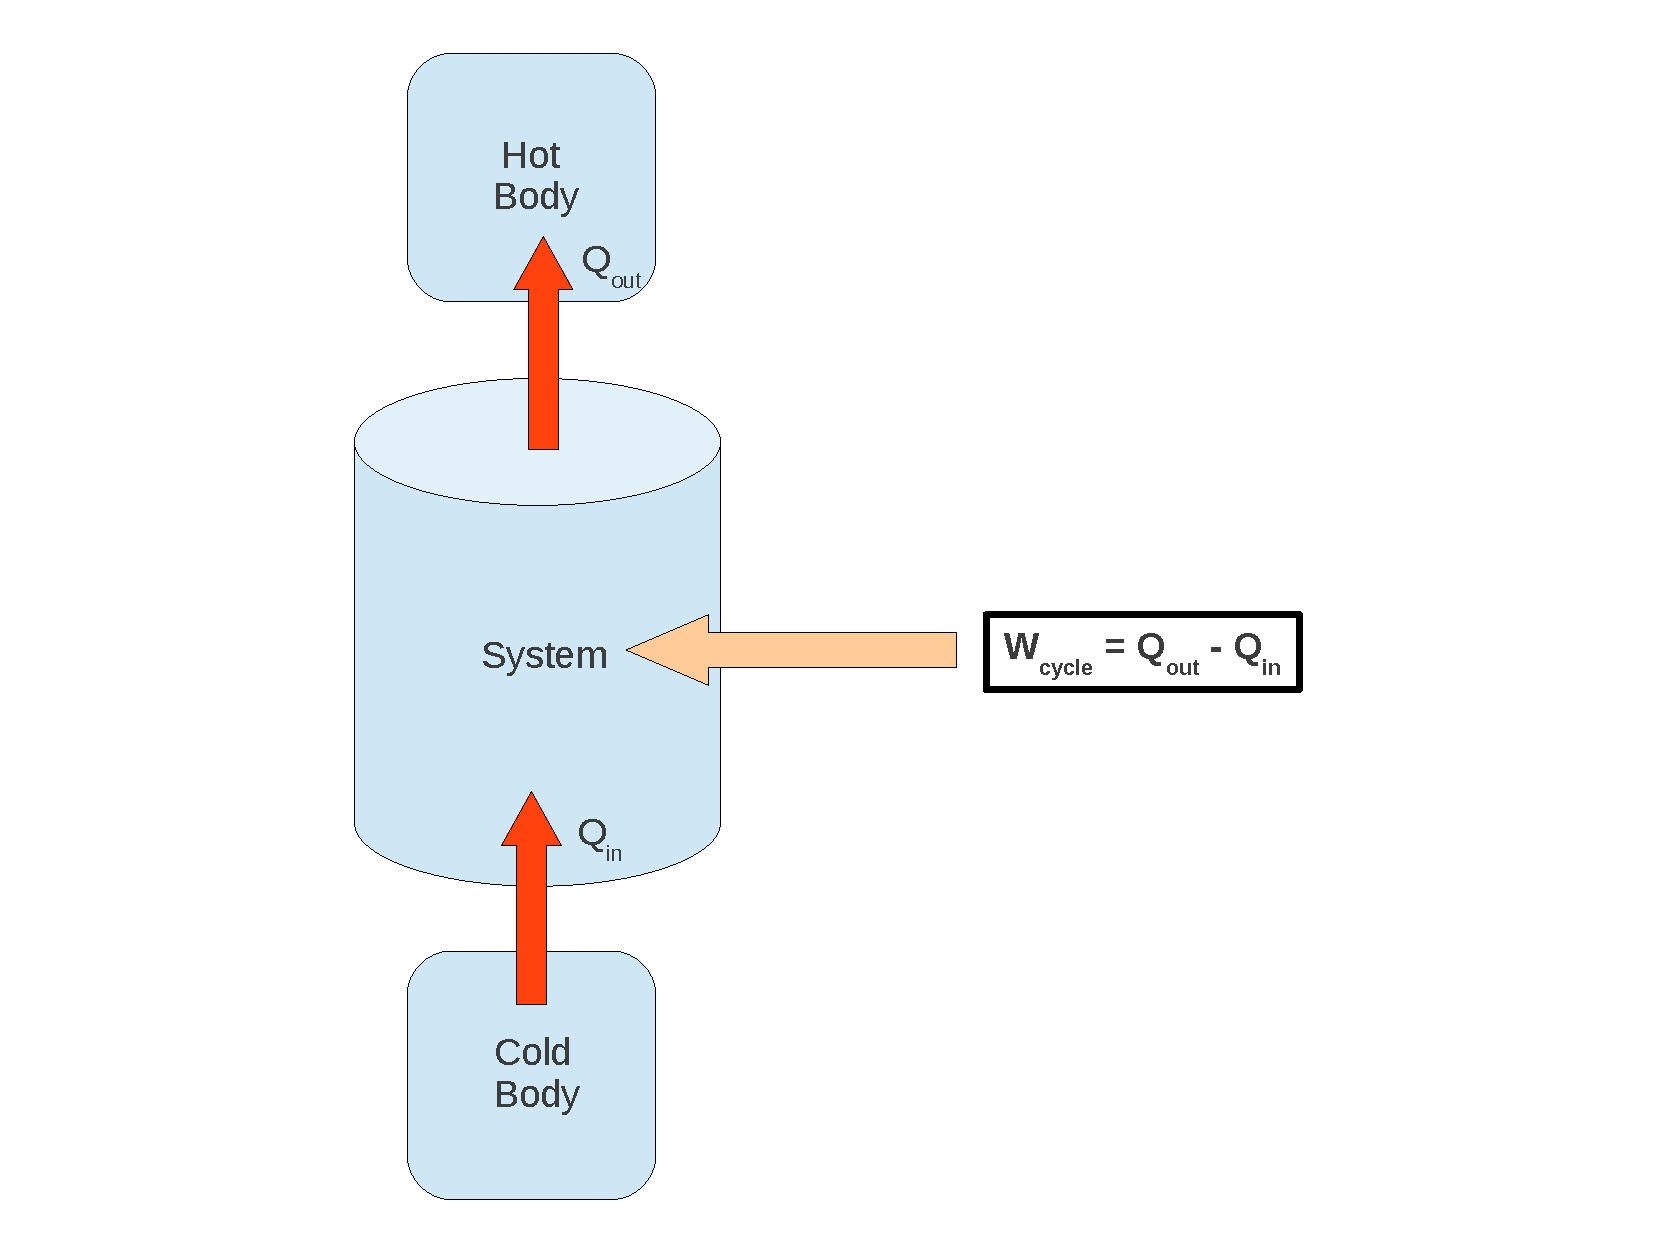
\includegraphics[width=8.cm,clip]{./Pics/FirstLaw_Cycle_02}
    \end{center}
   \end{figure}    
  \end{column}
 \end{columns}
 \normalsize
\end{frame}


%%%
%%% Slide
%%%
\begin{frame}
 \frametitle{Representations of the First Law -- Cycle}
 \begin{columns}
  \begin{column}[l]{0.5\linewidth}
   \begin{itemize}
    \item <1-> \textcolor{blue}{Heat pump cycle}:
     \begin{enumerate}[(a)]
      \item <2-> Objective: to maintain a heated space at a high temperature by absorbing heat from a low-temperature source (e.g., well water or cold outside air), and supplying this heat to the high-temperature medium (e.g., house);
      \item <3-> Coefficient of Performance: $\gamma = \displaystyle\frac{Q_{out}}{W_{cycle}} = \displaystyle\frac{Q_{out}}{Q_{out} - Q_{in}} = \beta + 1 \geq 1$;
      \item <4-> E.g., a fridge in a window (with the door open to cold outside environment): outside surrounding air $\xrightarrow{Q_{in}}$ refrigerant fluid $\left(T_{fluid} < T_{cavity}\right)$ $\xrightarrow{Q_{out}}$ inside the house; 
     \end{enumerate}
   \end{itemize}
  \end{column}
   
  \begin{column}[c]{0.5\linewidth}
   \begin{figure}%
    \begin{center}
     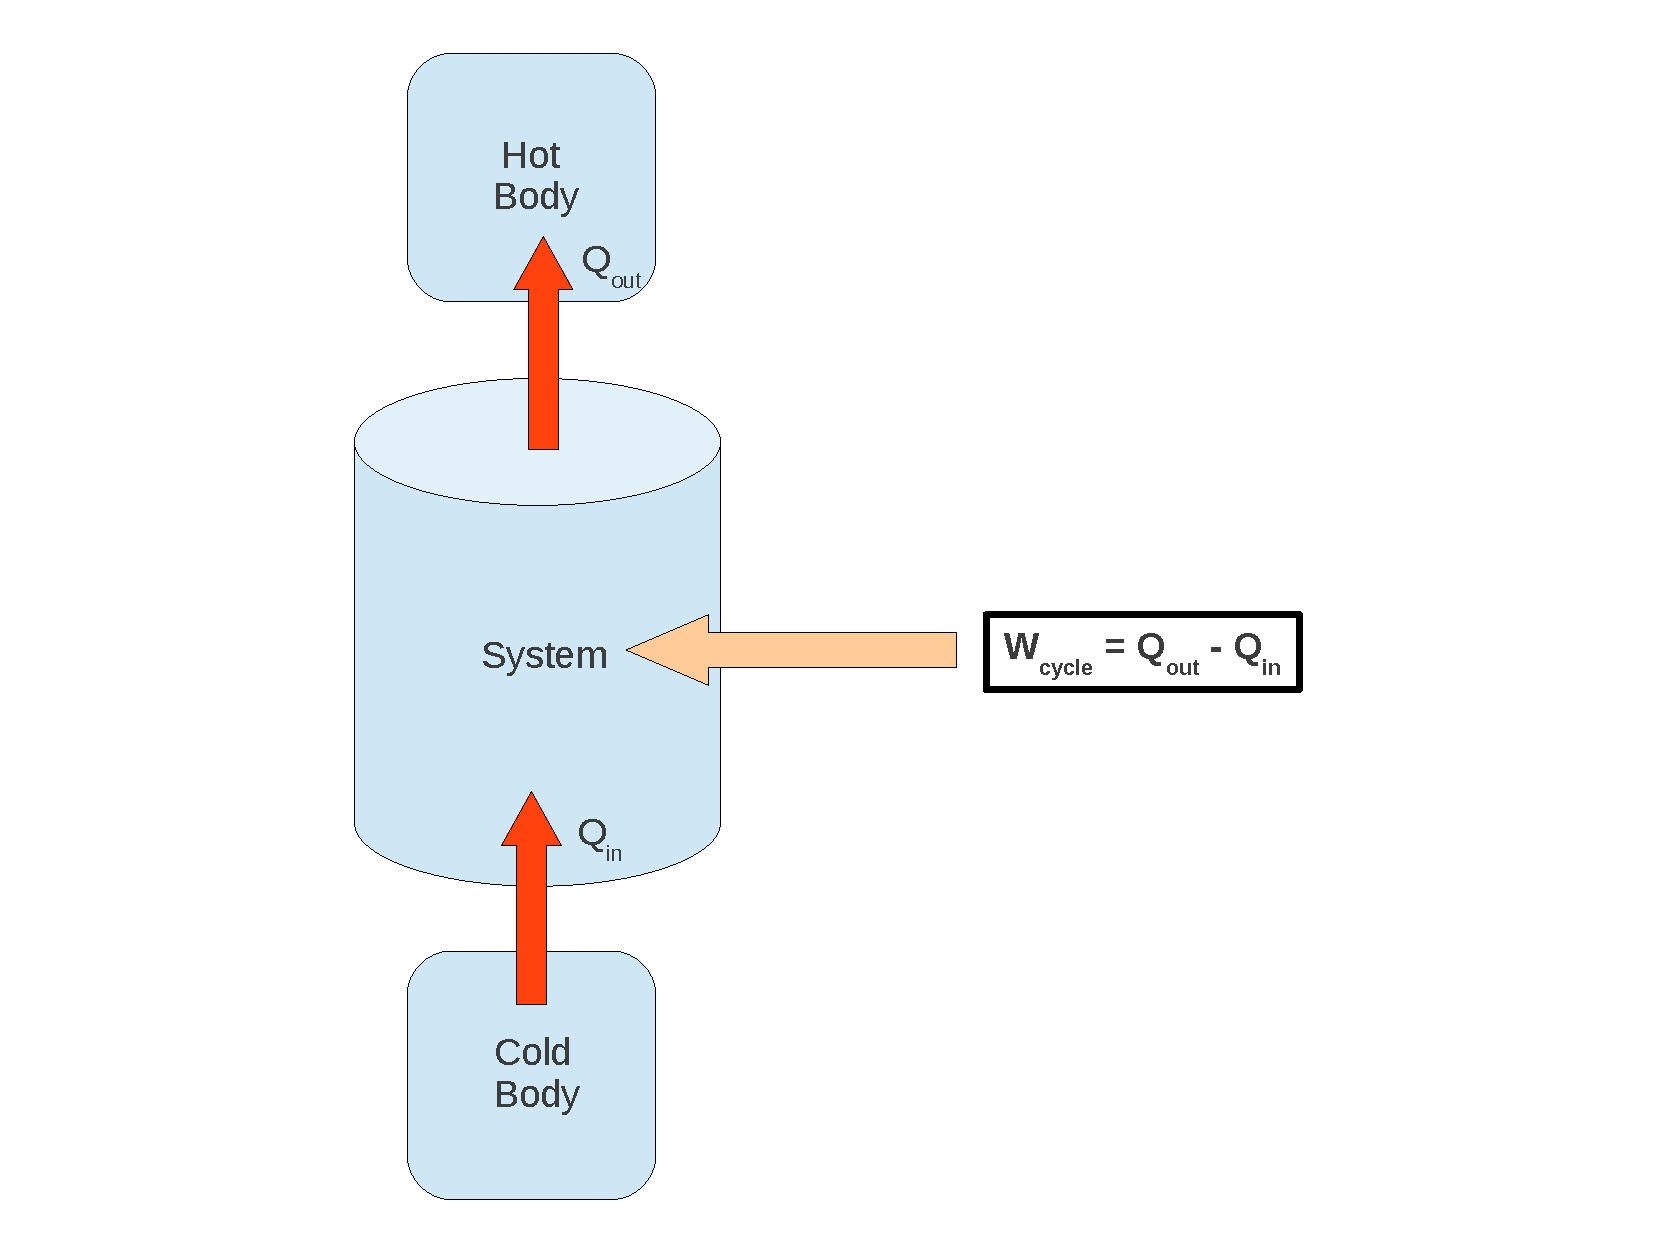
\includegraphics[width=8.cm,clip]{./Pics/FirstLaw_Cycle_02}
    \end{center}
   \end{figure}    
  \end{column}
 \end{columns}
 \normalsize
\end{frame}

%%%
%%% Slide
%%%
\begin{frame}
 \frametitle{Example 1: Thermodynamic Cycle}
   \textcolor{blue}{{\it {\bf Example:} A gas undergoes a thermodynamic cycle consisting of three processes: 
   \begin{enumerate}[(a)]
    \item \textcolor{blue}{{\it 1-2}: compression with $PV$ = constant, from $P_{1}$ = 1 bar, V$_{1}$ = 1.6m$^{3}$ to V$_{2}$ = 0.2m$^{3}$, U$_{2}$ - U$_{1}$ = 0.0 J;}
    \item \textcolor{blue}{{\it 2-3}: constant pressure to V$_{3}$ = V$_{1}$;}
    \item \textcolor{blue}{{\it 3-1}: constant volume, U$_{1}$ - U$_{3}$ = -3549 kJ.}
   \end{enumerate}
   There are no significant changes in kinetic or potential energy. Determine the heat transfer and work for process 2–3 (in kJ). Is this a power cycle or a refrigeration cycle?}}

   Let's assume that the gas is a closed system and the only work done is due to volume change. In order to compute the work for process {\it 2-3} with constant pressure,\\
   %\begin{displaymath}
    $W_{2}^{3} = \int\limits_{V_{2}}^{V_{3}} P dV = P_{2}\left(V_{3}-V_{2}\right)$\\
   %\end{displaymath}
   Using the {\it PV} relation for process {\it 1-2} $\rightarrow$ $P_{2}=P_{1}V_{1}V_{2}^{-1}=8\text{ bar}$. Thus , with $V_{3}=V_{1}$,\\
   $W_{2}^{3} = ( 8 bar ) \left[ \left( 1.6m^{3}\right) - \left( 0.2m^{3}\right) \right]$\\
   $\;\;\;\;\;\; = 11.2 \;bar.m^{3} \left[\textcolor{blue}{\frac{10^{5}N.m^{-2}}{1\; bar}\frac{1\; J}{1\; N.m}\frac{1\; kJ}{10^{3}\; J}}\right]= \textcolor{red}{1120 kJ}$
 \normalsize
\end{frame}


%%%
%%% Slide
%%%
\begin{frame}
 \frametitle{Example 1: Thermodynamic Cycle}

   The energy balance for process {\it 2-3} reduces to $Q_{2}^{3}=\left(U_{3}-U_{2}\right)+W_{2}^{3}$. \\
   Remember that in a cycle, $\left(\Delta U\right)_{\text{cycle}}=0$, therefore:\\
   $\left(U_{2}-U_{1}\right) + \left(U_{3}-U_{2}\right) + \left(U_{1}-U_{3}\right)=0$\\
   $\left(U_{3}-U_{2}\right) = - \left(U_{1}-U_{3}\right) = 3549 kJ$\\
   For process {\it 2-3}: $Q_{2}^{3}= 3549 + 1120 = \textcolor{red}{4669 kJ}$\\
\medskip

   For process {\it 1-2}: $\Delta U = 0$, \\
   $Q_{1}^{2} = W_{1}^{2} = \int_{V_{1}}^{V_{2}}P dV = P_{1}V_{1}\ln\left(V_{2}/V_{1}\right) $\\
   $\;\;\;\;\;=\textcolor{red}{-332.7 kJ}$\\
\medskip

   And for process {\it 3-1}: $W_{3}^{1}=0$ and $Q_{3}^{1}=U_{1}-U_{3}=\textcolor{red}{-3549 kJ}$. The cycle can then be calculated as,
   $W_{\text{cycle}}=W_{1}^{2}+W_{2}^{3}+W_{3}^{1} = -332.7 + 1120 + 0 = 787.3 kJ$\\

\medskip
   Since \textcolor{red}{$W_{\text{cycle}}>0$}, the cycle is a \textcolor{red}{power cycle}.
 \normalsize
\end{frame}

%%%
%%% Slide
%%%
\begin{frame}
 \frametitle{Representations of the First Law -- Process}

   Let's consider the set of paths from state 1 to 2:
   \begin{itemize}
    \item Cycle I: 1 to 2 on Path A followed by 2 to 1 on Path B;
    \item Cycle II: 1 to 2 on Path A followed by 2 to 1 on Path C;
   \end{itemize}

   \begin{figure}%
    \begin{center}
     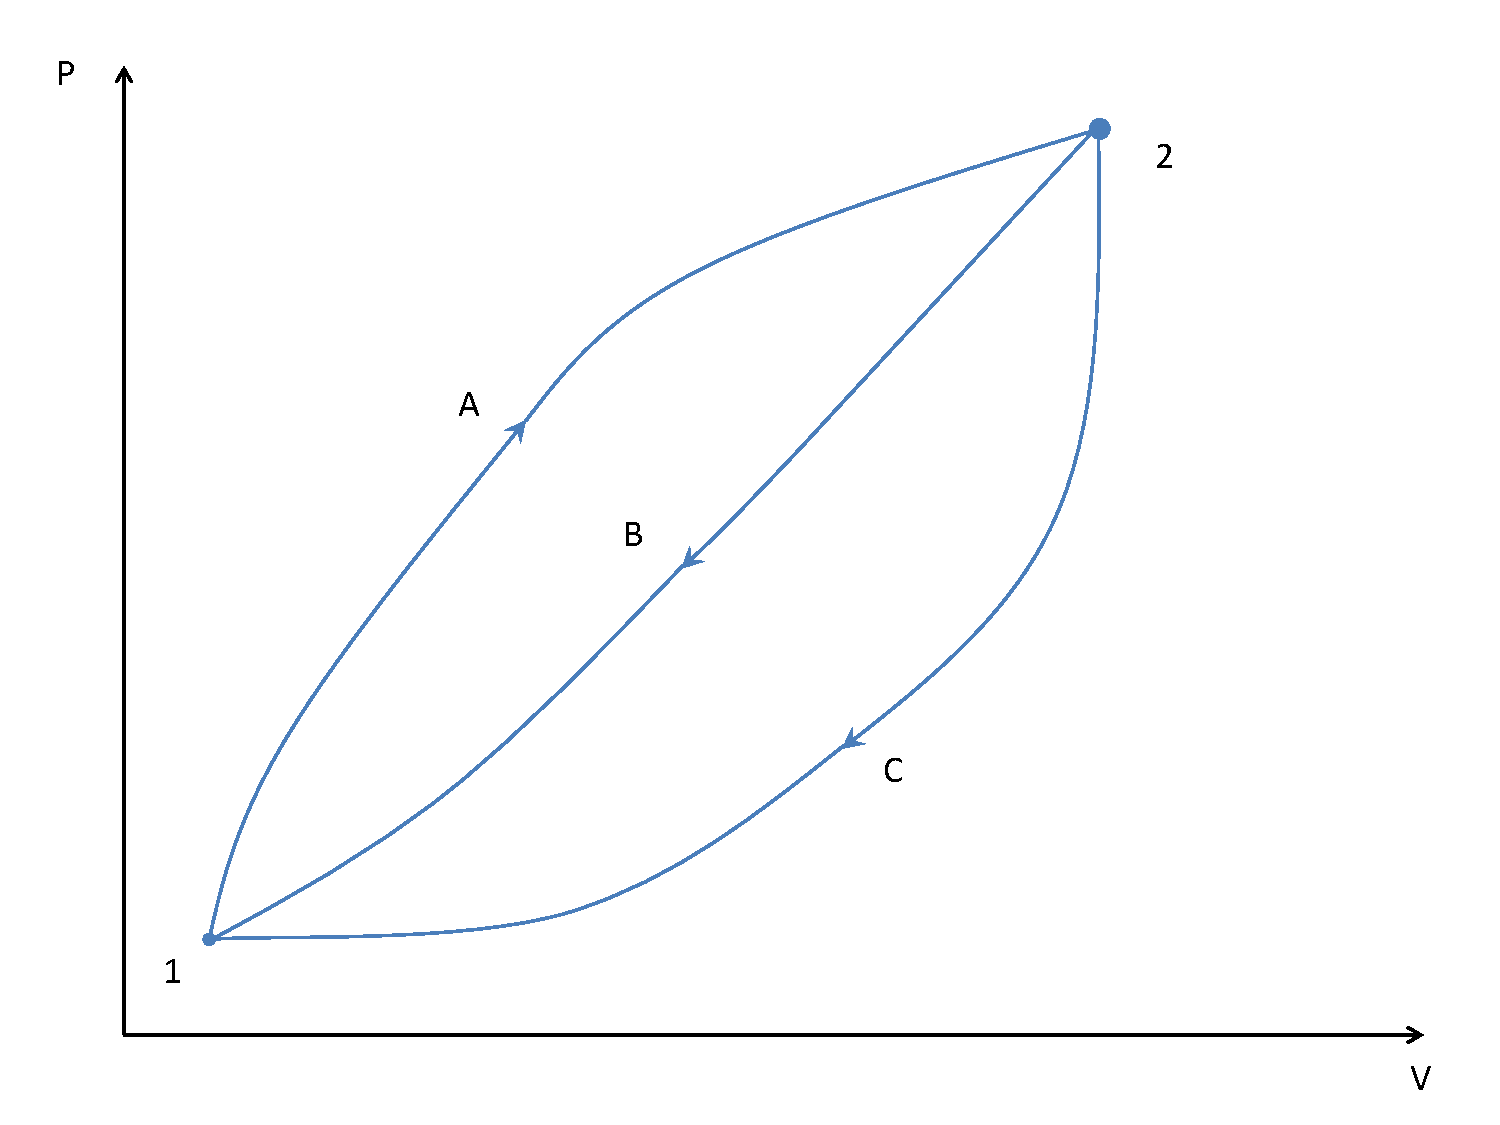
\includegraphics[width=7.5cm,clip]{./Pics/first_law_process}
     %\caption{P-V diagram for various combinations of processes forming cyclic integrals.}
    \end{center}
   \end{figure}

\normalsize
\end{frame}


%%%
%%% Slide
%%%
\begin{frame}
 \frametitle{Representations of the First Law -- Process}
   \begin{itemize}
    \item <1-> These cycles can be mathematically represented using Eqn. \ref{Module00:first_law}:
   \begin{eqnarray}
    \text{Cycle I:}  \int\limits_{1}^{2}\delta Q_{A} + \int\limits_{2}^{1}\delta Q_{B} = \int\limits_{1}^{2}\delta W_{A} + \int\limits_{2}^{1}\delta W_{B}  \label{Module00:proc1a}\\
    \text{Cycle II:} \int\limits_{1}^{2}\delta Q_{A} + \int\limits_{2}^{1}\delta Q_{C} = \int\limits_{1}^{2}\delta W_{A} + \int\limits_{2}^{1}\delta W_{C}  \label{Module00:proc1b}
   \end{eqnarray}
   \item <2-> Subtracting \ref{Module00:proc1b} from \ref{Module00:proc1a} and rearranging:
   \begin{equation}
    \int\limits_{2}^{1}\left(\delta Q- \delta W\right)_{B} = \int\limits_{2}^{1}\left(\delta Q- \delta W\right)_{C}\label{Module00:proc1c}
   \end{equation}
   \item <3-> B and C are arbitrary paths ; Eqn. \ref{Module00:proc1c} asserts that the integral of $\left(\delta Q -\delta W\right)\left.\right|_{2}^{1}$ is path-independent. Notice, however that both \textcolor{blue}{Q} and \textcolor{blue}{W} are path-dependent quantities. 
    \end{itemize}
\end{frame}



%%%
%%% Slide
%%%
\begin{frame}
 \frametitle{Representations of the First Law -- Process}

  \begin{itemize}
   \item <1-> Energy (as any property) depends only on the state and not the path taken to arrive at the state. Defining the differential of U:\\
    $dU =\delta Q - \delta W$\\ 
   
   \item <2-> Integrating from 1 to 2:\\
    $\displaystyle\int\limits_{1}^{2}dU =\displaystyle\int\limits_{1}^{2}\delta Q - \displaystyle\int\limits_{1}^{2}\delta W$\\ 

   \item <3-> Leading to
   \begin{equation}
    U_{2} - U_{1} = Q_{1}^{2}- W_{1}^{2} \label{Module00:proc1a}
   \end{equation}

  \end{itemize}
\normalsize
\end{frame}



%%%
%%% Slide
%%%
\begin{frame}
 \frametitle{Representations of the First Law -- Process}
 \begin{block}{Another way to state the First Law} 
  For a system undergoing a process, the change in energy is equal to the heat added to the system minus the work done by the system.
  \begin{displaymath}
   dU =\delta Q - \delta W 
  \end{displaymath}
 \end{block}
\end{frame}


%%%
%%% Slide
%%%
\begin{frame}
 \frametitle{Example 2: Conservation of Work}
 \scriptsize
 \begin{columns}
  \begin{column}[r]{0.5\linewidth}
   \begin{figure}%
    \begin{center}
     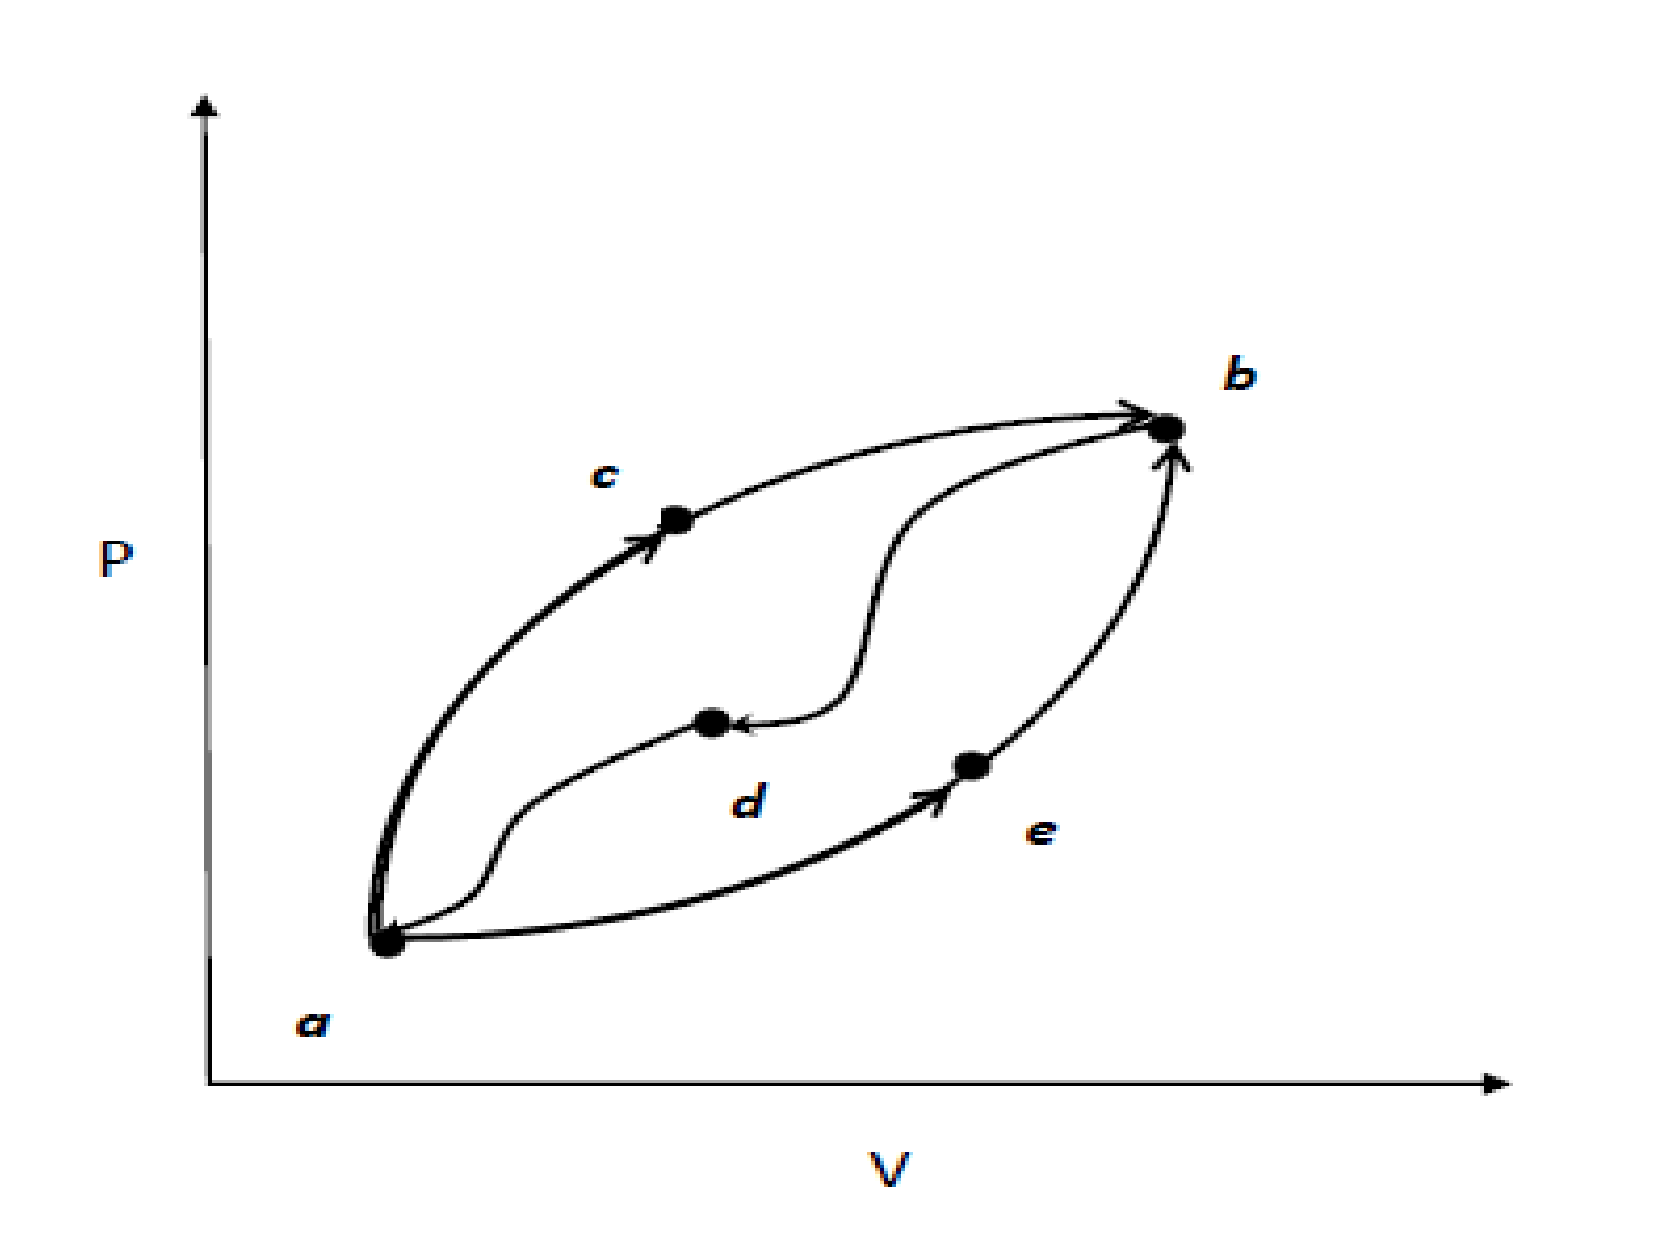
\includegraphics[width=\columnwidth,clip]{./Pics/First_Law_1}
    \end{center}
   \end{figure}
  \end{column}
  \begin{column}[r]{0.5\linewidth}
   When a system is taken from state \textcolor{blue}{a} to state \textcolor{blue}{b} along path \textcolor{blue}{acb}, 100 J of heat flows into the system and the system does 40 J of work. 
   \begin{itemize}
    \item<2-> How much heat flows into the system along path \textcolor{blue}{aeb} if the work done by the system is 20 J?\\
          For path \textcolor{blue}{acb}:
          \begin{displaymath}
           \Delta U_{ab} = Q_{acb}-W_{acb} = 100 - 40 = 60 J
          \end{displaymath}
          For path \textcolor{blue}{aeb}:
          \begin{eqnarray}
           &&\Delta U_{ab} = Q_{aeb}-W_{aeb} = 60 J \nonumber \\
           &&\Delta U_{ab} = Q_{aeb}-20 \therefore Q_{aeb} = 80 J \nonumber
          \end{eqnarray}
    \item<3-> The system returns from \textcolor{blue}{b} to \textcolor{blue}{a} along path \textcolor{blue}{bda}. If the work done on the system is 30 J, does the system absorb or liberate heat? How much? \\
           For path \textcolor{blue}{bda}: 
           \begin{eqnarray}
            &&\Delta U_{ba} = -60 J = Q_{bda}-W_{bda} \nonumber \\
            &&\Delta U_{ba} = Q_{bda} + 30 \therefore Q_{bda} = -90 J \nonumber
           \end{eqnarray}
   \end{itemize}
  \end{column}
 \end{columns}
\normalsize
\end{frame}


%%%
%%% Slides
%%%
\begin{frame}
 \frametitle{Reversible Processes}
   \begin{itemize}
    \item When an object at temperature $T=T\left(t_{0}\right)$ is left in a room in contact with ambient air, it is intuitive that the object will cool down at time $t_{1}$ and the air will warm up until the temperature of the body and the surrounding air are the same;
    \item From the First Law, we know that the {\it decrease in the internal energy of the body is equal to the increase in the internal energy of the surrounding air};
    \item The body cools down spontaneously and we can predict the {\it direction} of the process as it moves towards an equilibrium state, but; 
   \end{itemize}
    \begin{figure}%
     \begin{center}
      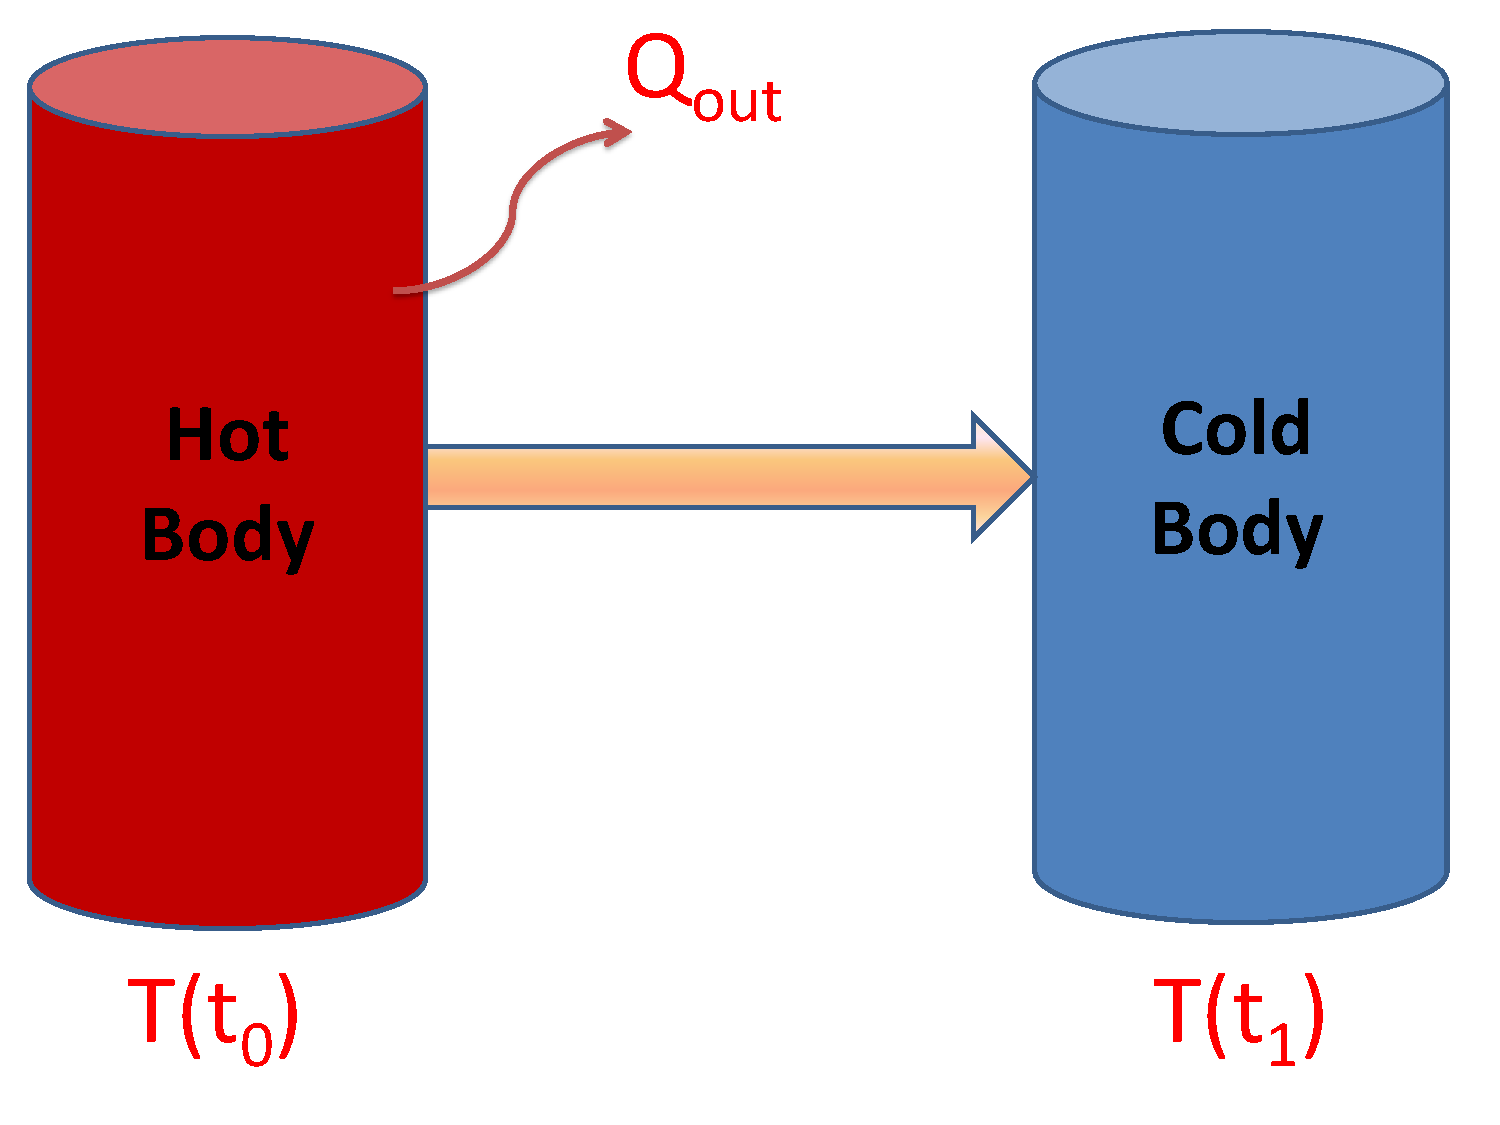
\includegraphics[width=5.5cm,clip]{./Pics/HotColdCoffee}
     \end{center}
    \end{figure}
 \normalsize
\end{frame}


%%%
%%% Slides
%%%
\begin{frame}
 \frametitle{Reversible Processes}
   \begin{itemize}
    \item The initial state $\left(\text{i.e., }T_{0}\right)$ can be restored {\it but not spontaneously} $\Longrightarrow$  The reverse processes do not violate the First Law, and yet they {\it do not occur spontaneously};
    \item Another law is needed to help understand and predict which processes will occur spontaneously.
   \end{itemize}
    \begin{figure}%
     \begin{center}
      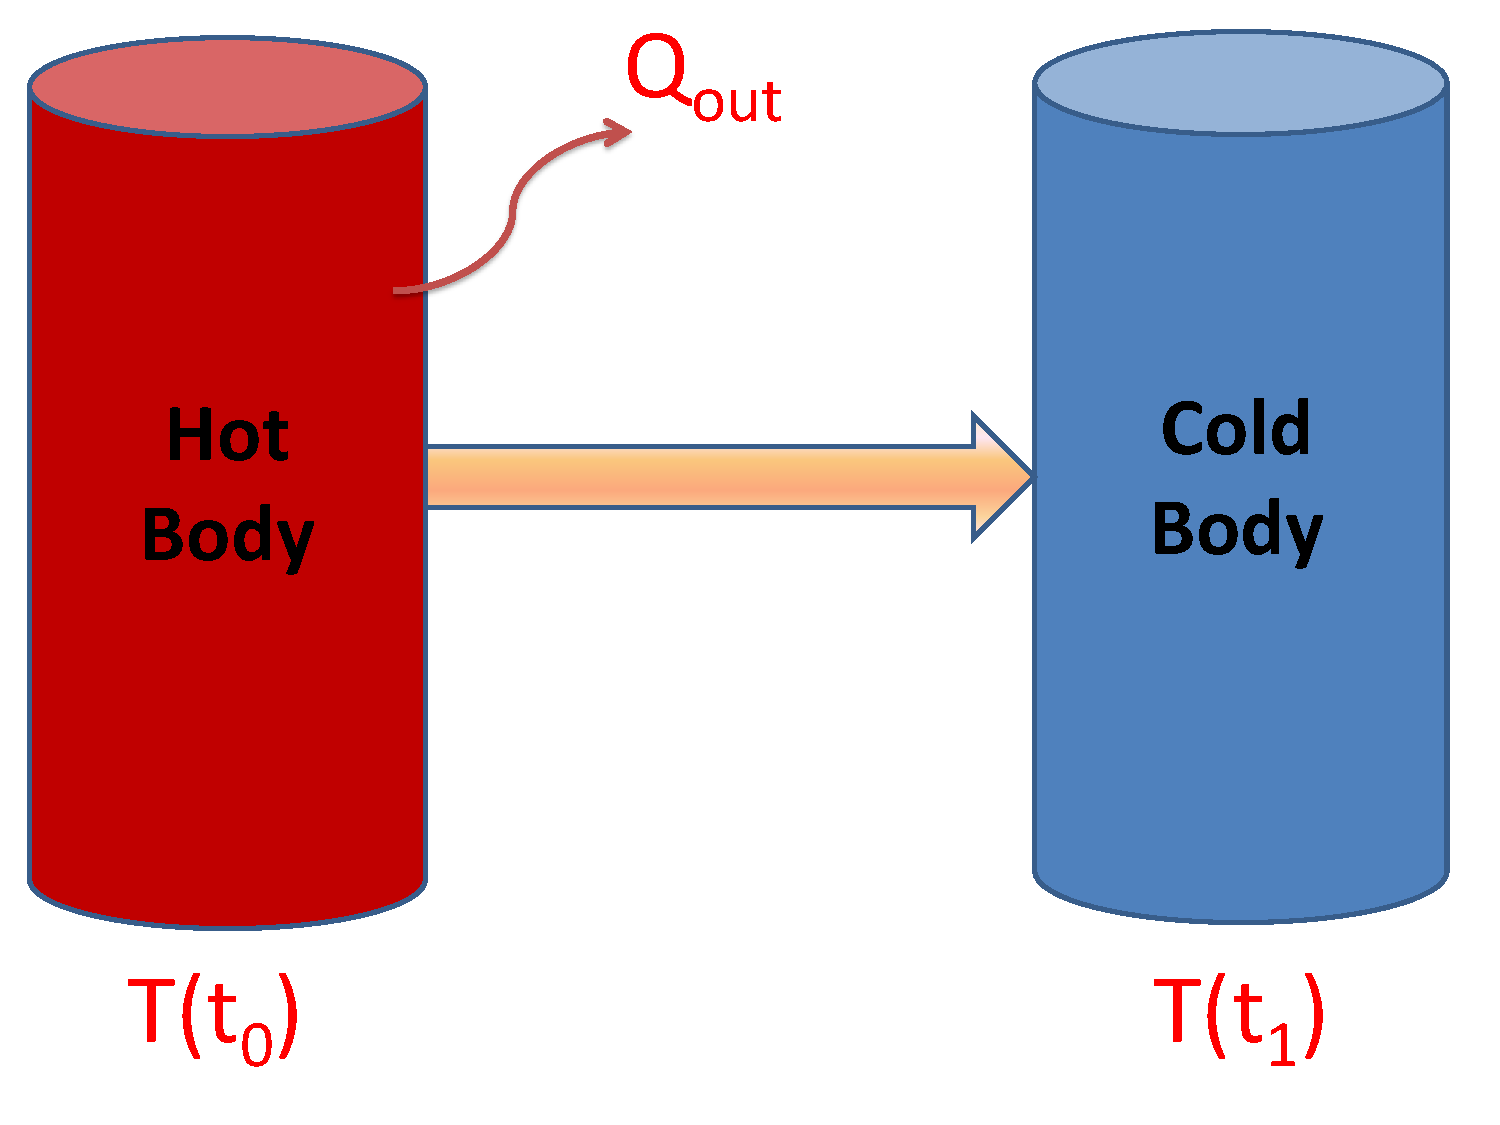
\includegraphics[width=5.5cm,clip]{./Pics/HotColdCoffee}
     \end{center}
    \end{figure}
 \normalsize
\end{frame}


%%%
%%% Slides
%%%
\begin{frame}
 \frametitle{Reversible Processes}
 \begin{itemize}
  \item <2-> \textcolor{blue}{Reversible process:} A process in which it is possible to return both the system and surroundings to their original states;
  \item <3-> \textcolor{blue}{Irreversible process:} A process in which it is impossible to return both the system and surroundings to their original states.
 \end{itemize}

\end{frame}

%%%
%%% Slides
%%%
\begin{frame}
 \frametitle{Isochoric and Isobaric Processes}
     \visible<1->{\begin{block}{Energy conservation in a closed system:}
       $d U^{t}=d Q + d W$ \hspace{2cm} $d W = -P dV^{t}$ \hspace{2cm} $d U^{t}=d Q -P d V^{t}$
    \end{block}}

    \visible<2->{\begin{block}{Constant volume process (isochoric):}
       $-P d V^{t} =0$ \hspace{3cm} $d U^{t} = d Q$ \hspace{3cm} $\Delta U^{t}= Q $
    \end{block}}

    \visible<3->{\begin{block}{Constant pressure process (isobaric):}
       $d Q = d U^{t} + d\left(P V^{t}\right)= d\left(U^{t}+PV^{t}\right)$ \hspace{3cm} $H = U + PV$
    \end{block}}
 
 \normalsize
\end{frame}


%%%
%%% Slides
%%%
\begin{frame}
 \frametitle{Heat Capacity}
     \begin{itemize}
        \item<1-> General definition:
          \visible<1->{\begin{displaymath}
            C = \frac{dQ}{dT}
          \end{displaymath}}
        \item<2-> At \textcolor{blue}{constant volume}
             \visible<2->{\begin{displaymath}
                C_{V} = \left(\frac{\partial U}{\partial T}\right)_{V} \Longleftrightarrow  Q = n\Delta U = n\int\limits_{T_{1}}^{T_{2}} C_{V} dT
             \end{displaymath}}
        \item<3-> At \textcolor{blue}{constant pressure}
             \visible<2->{\begin{displaymath}
                C_{P} = \left(\frac{\partial H}{\partial T}\right)_{P} \Longleftrightarrow  Q = n\Delta H = n\int\limits_{T_{1}}^{T_{2}} C_{P} dT
             \end{displaymath}}
     \end{itemize}
 
 \normalsize
\end{frame}


%%%
%%% Slides
%%%
\begin{frame}
 \frametitle{Open Systems}
     \begin{itemize}
        \item<1-> Control volume and flow rates:
         \visible<1->{
         \begin{center}
           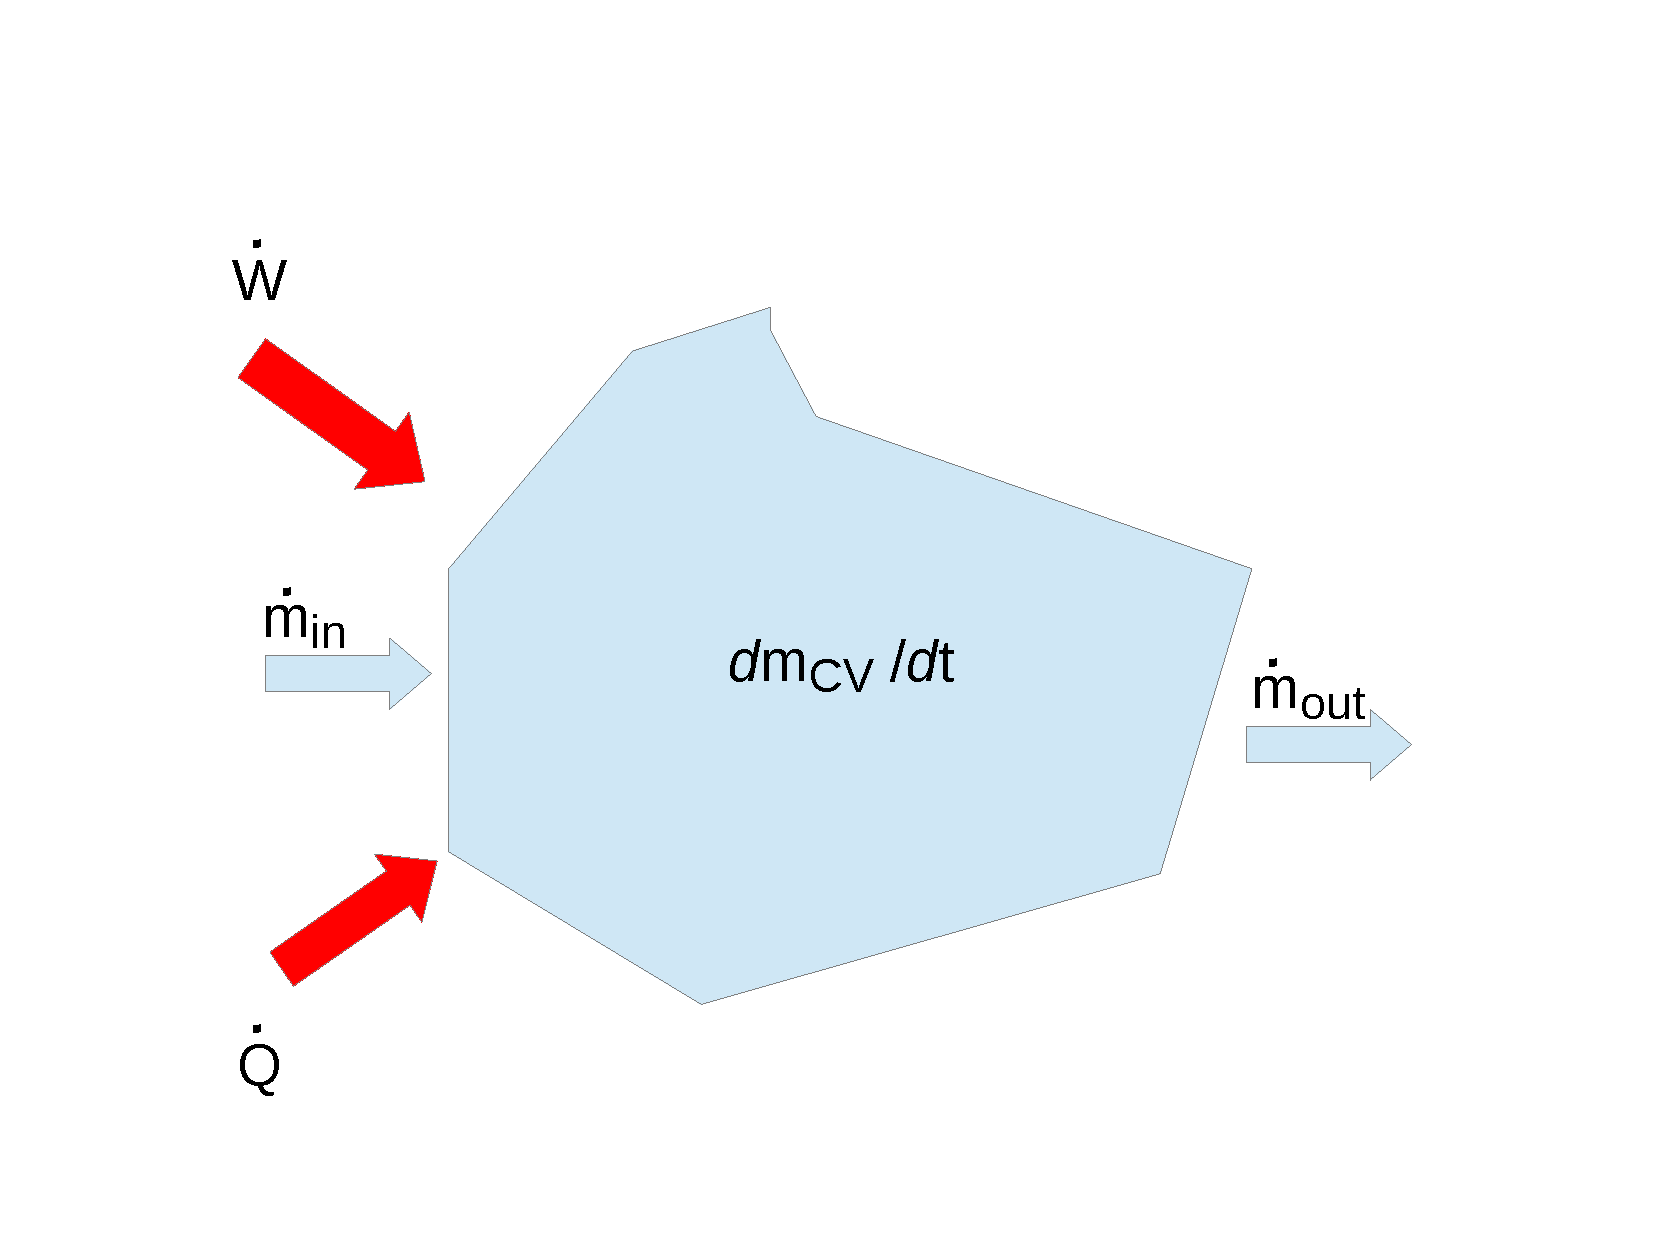
\includegraphics[width=6.cm,clip]{./Pics/Energy_OpenedSystems}
         \end{center}}
        \item<2-> Mass balance:
             \visible<2->{\begin{displaymath}
                \frac{d m_{cv}}{dt}+ \left(\dot{m}_{out}-\dot{m}_{in}\right) = 0
             \end{displaymath}} 
     \end{itemize}
 
 \normalsize
\end{frame}

%%%
%%% Slides
%%%
\begin{frame}
 \frametitle{Open Systems}
     \begin{itemize}
        \item<1-> Energy balance:
           \visible<1->{\begin{displaymath}
             \frac{d\left(m U\right)_{cv}}{d t} + \Delta\left[\left(H + \frac{1}{2}u^{2} + z g\right)\dot{m}\right]=\dot{Q}+\dot{W}
           \end{displaymath}} 
        \item<2-> Steady-state flow process:
           \visible<2->{\begin{eqnarray}
             && \cancelto{0}{\frac{d\left(m U\right)_{cv}}{d t}} + \Delta\left[\left(H + \frac{1}{2}u^{2} + z g\right)\dot{m}\right]=\dot{Q}+\dot{W} \nonumber \\
             && \textcolor{blue}{\Delta H + \frac{\Delta u^{2}}{2} +g\Delta z= Q + W} \nonumber 
           \end{eqnarray}}          
     \end{itemize}
 
 \normalsize
\end{frame}


%%%
%%% Slides
%%%
\begin{frame}
 \frametitle{Ideal Gas: General Remarks}
     \begin{enumerate}
        \item<1-> Equation of state:
           \visible<1->{\begin{displaymath}
              P V = R T
           \end{displaymath}} 
        \item<2-> Heat capacity ratios:
           \visible<2->{\begin{eqnarray}
             && C_{V}=\left(\frac{\partial U}{\partial T}\right)_{V} = \frac{d U(T)}{d T} = C_{V}(T) \nonumber \\
             && C_{P}=\left(\frac{\partial H}{\partial T}\right)_{P} = \frac{d H(T)}{d T} = C_{P}(T) \nonumber
           \end{eqnarray}}    
        \item<3-> Internal energy {\bf depends only on} the temperature, $U = U(T)$;    
        \item<4-> Formally defining {\it Enthalpy}:
           \visible<4->{\begin{displaymath}
              H \equiv U + PV = U(T) + RT = H(T)
           \end{displaymath}} 
        \item<5-> Relationship between $C_{P}(T)$ and $C_{V}(T)$:
           \visible<5->{\begin{displaymath}
              C_{P}=\frac{d H(T)}{d T} = \frac{d U(T)}{d T} + \frac{d(RT)}{d T} = C_{V} + R
           \end{displaymath}}           
     \end{enumerate} 
  \normalsize
\end{frame}


%%%
%%% Slides
%%%
\begin{frame}
 \frametitle{Ideal Gas: Processes}
     \begin{enumerate}
        \item<1-> Processes involving {\it heat} and {\it work} quantities:
           \visible<1->{\begin{eqnarray}
             && d Q = C_{V} dT + RT \frac{d V}{V}  \Longleftrightarrow dW = -RT\frac{d V}{V} \nonumber \\
             && d Q = C_{P} dT - RT \frac{d P}{P}  \Longleftrightarrow dW = -R d T + RT\frac{d P}{P} \nonumber
           \end{eqnarray}} 
        \item<2-> With $PV = RT$
           \visible<2->{\begin{displaymath}
              d W = -P d V  \Longleftrightarrow dQ = \frac{C_{V}}{R}VdP + \frac{C_{P}}{R}P d V  
           \end{displaymath}}    
     \end{enumerate} 
  \normalsize
\end{frame}


%%%
%%% Slides
%%%
\begin{frame}
 \frametitle{Ideal Gas: Processes}
     \begin{enumerate}  \setcounter{enumi}{2}
        \item<1-> Isothermal procesess $(dT = 0)$:
           \visible<1->{\begin{displaymath}
              Q = -W = RT \ln\frac{V_{2}}{V_{1}} = -RT \ln\frac{P_{2}}{P_{1}}
           \end{displaymath}} 
        \item<2-> Isobaric process $(dP= 0)$:
           \visible<2->{\begin{displaymath}
              Q = \Delta H = \int\limits_{T_{1}}^{T_{2}}C_{P}dT
           \end{displaymath}}    
        \item<3-> Isochoric process $(dV= 0)$:
           \visible<3->{\begin{displaymath}
              Q = \Delta U = \int\limits_{T_{1}}^{T_{2}}C_{V}dT
           \end{displaymath}}     
     \end{enumerate} 
  \normalsize
\end{frame}


%%%
%%% Slides
%%%
\begin{frame}
 \frametitle{Ideal Gas: Processes}
     \begin{enumerate}  \setcounter{enumi}{5}
        \item<1-> Adiabatic process $(dQ= 0)$:
           \visible<1->{\begin{displaymath}
               \frac{T_{2}}{T_{1}} = \left(\frac{V_{1}}{V_{2}}\right)^{\frac{R}{C_{V}}} \Leftrightarrow \frac{T_{2}}{T_{1}} = \left(\frac{P_{2}}{P_{1}}\right)^{\frac{R}{C_{P}}} \Leftrightarrow \frac{P_{2}}{P_{1}} = \left(\frac{V_{1}}{V_{2}}\right)^{\frac{C_{P}}{C_{V}}} 
           \end{displaymath}}    
         \item<2-> If we define $\gamma \equiv \displaystyle\frac{C_{P}}{C_{V}}$, the relations above can be rewritten as,
           \visible<2->{\begin{displaymath}
               TV^{\gamma-1}=\text{const.} \Leftrightarrow TP^{\frac{1-\gamma}{\gamma}}=\text{const.} \Leftrightarrow PV^{\gamma}=\text{const.} 
           \end{displaymath}}    
         \item<3-> And for {\it polytropic} processes,
           \visible<3->{\begin{displaymath}
               TV^{\delta-1}=\text{const.} \Leftrightarrow TP^{\frac{1-\delta}{\delta}}=\text{const.} \Leftrightarrow PV^{\delta}=\text{const.} 
           \end{displaymath}}    
     \end{enumerate} 
  \normalsize
\end{frame}


%%%
%%%  SUBSECTION
%%%
\subsection{Statements of the Second Law}

%%%
%%% Slides
%%%
\begin{frame}
 \frametitle{Second Law of Thermodynamics}
 %\scriptsize
 \begin{itemize}
   \item <2->The second law of thermodynamics is an expression of the tendency that over time, differences in temperature, pressure and chemical potential will reach an equilibrium state in an isolated physical system;
   \item <3->From the state of thermodynamic equilibrium, the law deduced the principle of the increase of entropy and explains the phenomenon of irreversibility.
 \end{itemize}

 \visible<4->{\begin{block}{R. Clausius  (1854)}
  \begin{center}
  \textcolor{blue}{$\lq$It is impossible to devise an engine which, working in a cycle, shall produce no effect other than the transfer of heat from a colder to hotter body.'}
  \end{center}
 \end{block}}

 \visible<5->{\begin{block}{Kelvin (1951) and Planck (1897)}
  \begin{center}
  \textcolor{blue}{$\lq$It is impossible to devise an engine which, working in a cycle, shall produce no effect other than the extraction of heat from a reservoir and the performance of an equal amount of mechanical work.'}
  \end{center}
 \end{block}}

 \normalsize
\end{frame}


%%%
%%% Slides
%%%
\begin{frame}
 \frametitle{Second Law of Thermodynamics}
 
   \begin{figure}%
    \begin{center}
     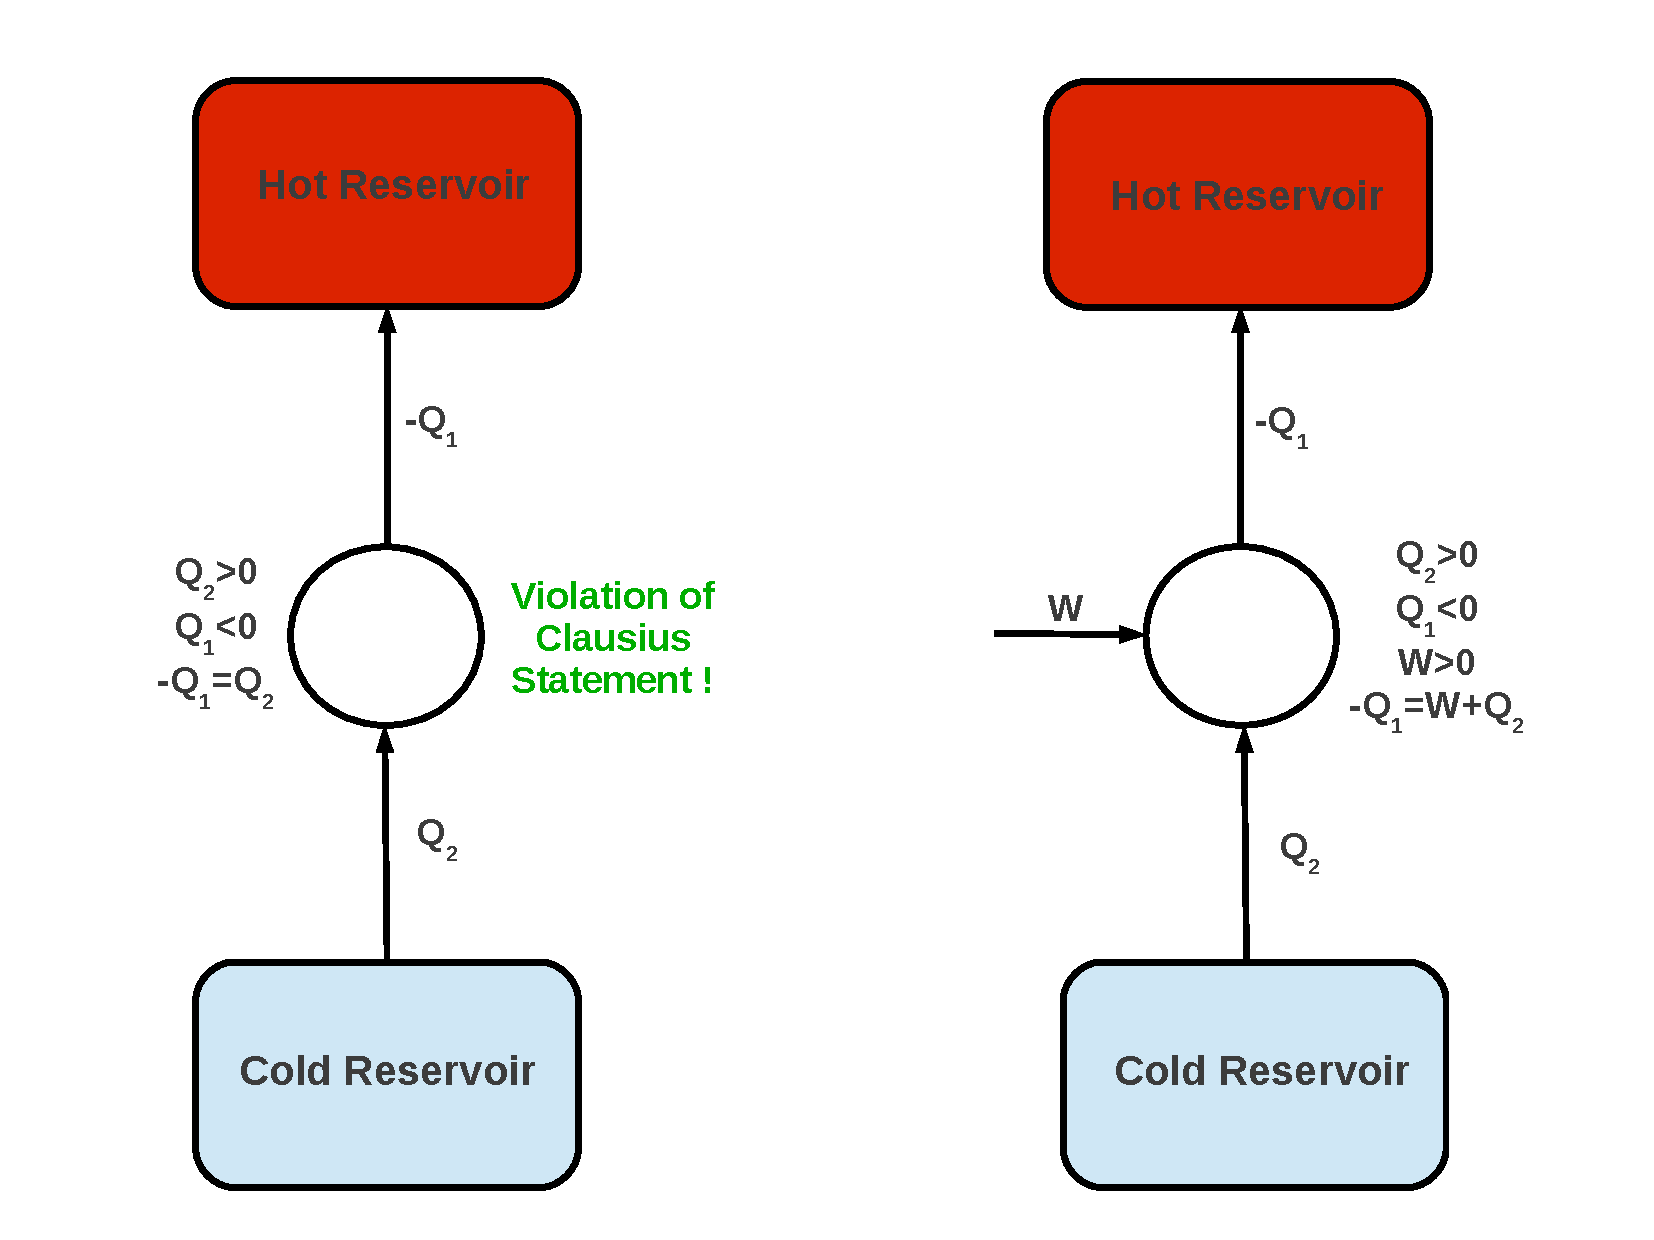
\includegraphics[width=8.cm,clip]{./Pics/2ndLaw_Schem}
    \end{center}
   \end{figure} 

   \begin{center}
     All spontaneous processes are irreversible -- heat flows from hot to cold spontaneously and irreversibly.
   \end{center}
   
\end{frame}

%%%
%%% Slides
%%%
\begin{frame}
 \frametitle{Derivation of the Mathematical Statement of the Second Law}
 %\scriptsize
 \begin{columns}

  \begin{column}[c]{0.5\linewidth}
   \begin{itemize}
    \item <2-> In the schematics (rhs), an infinitesimal amount of heat, $\delta Q^{\prime}$, is transferred from the thermal reservoir (with temperature $T_{res}$) to a reversible cyclic engine (1). 
    \item <3-> The engine produces a small amount of work, $\delta W^{\prime}$, and releases an infinitesimal amount of heat, $\delta Q$ to another reservoir at variable temperature $T$. 
    \item <4-> The second reservoir (2) also releases work $\left(\delta W\right)$ to the surroundings.
   \end{itemize}


  \end{column}

  \begin{column}[c]{0.5\linewidth}
   \begin{figure}%
    \begin{center}
     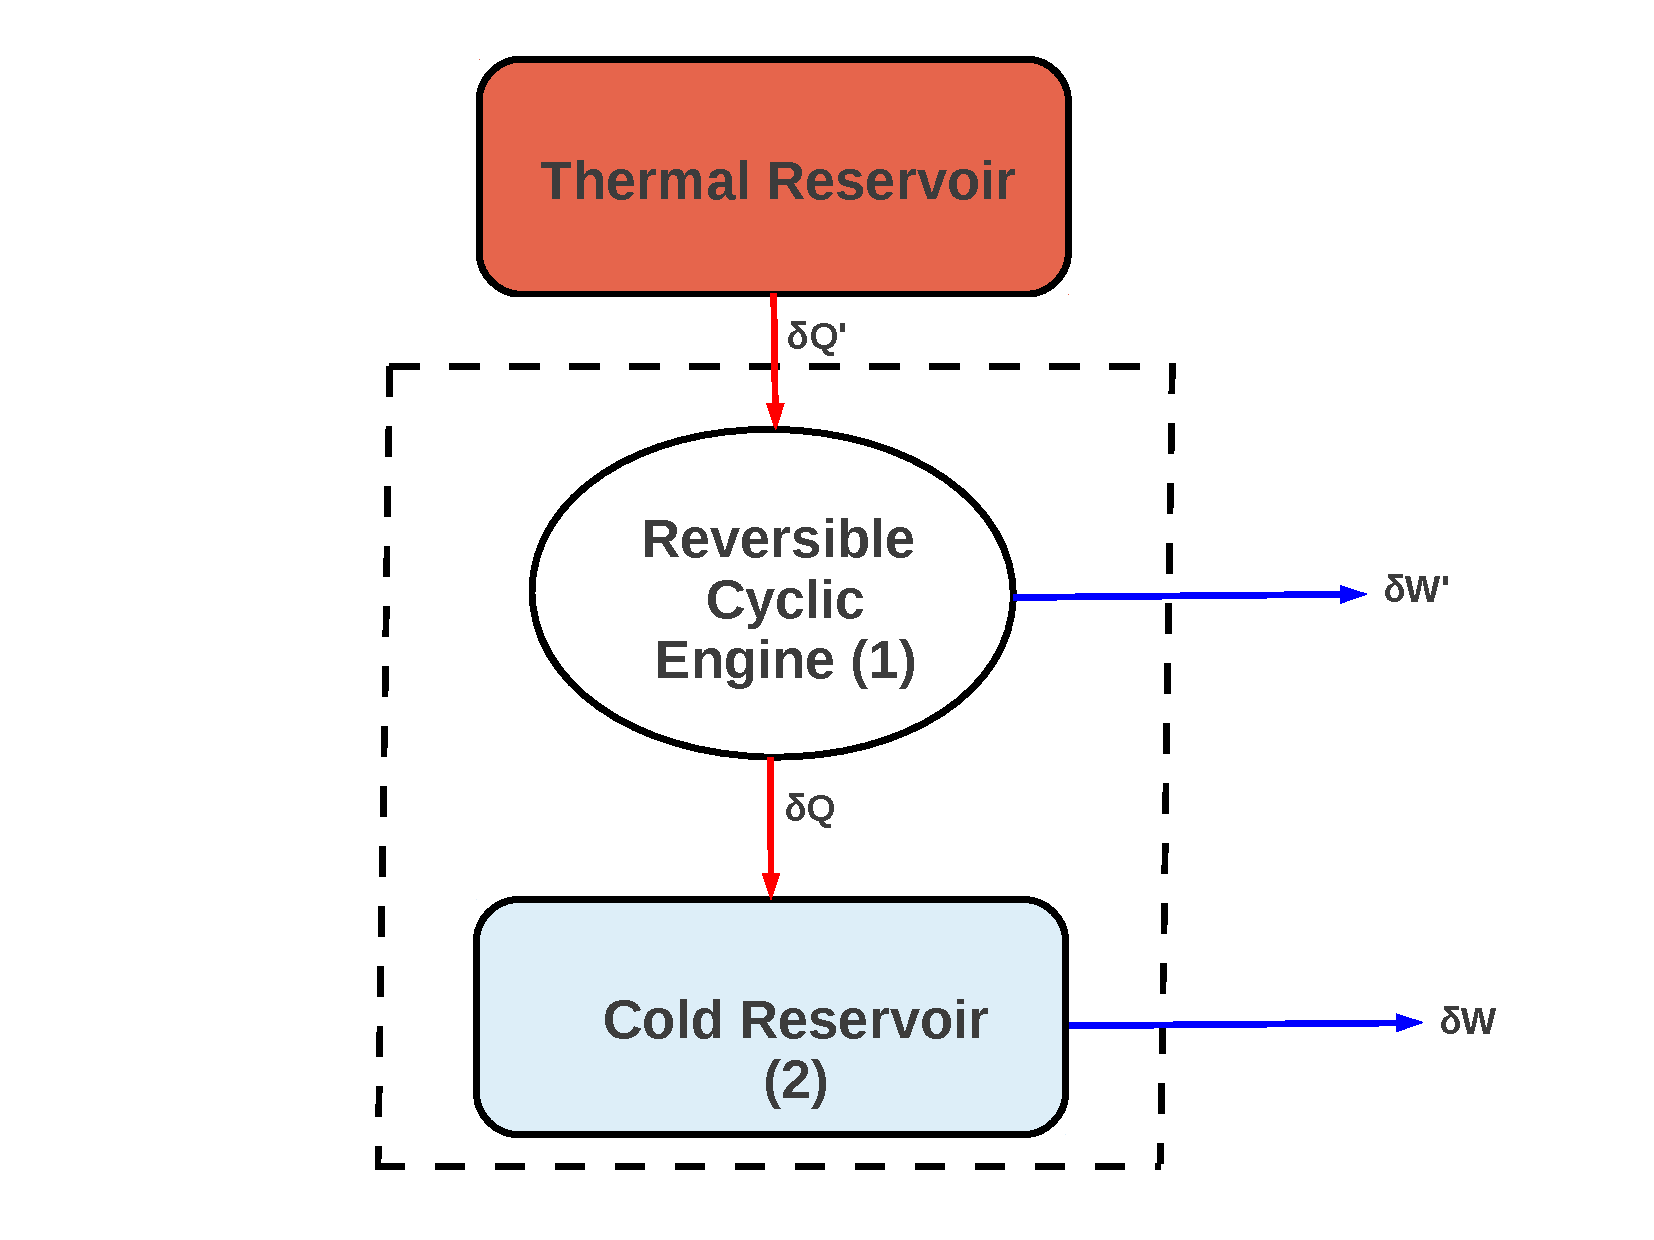
\includegraphics[width=1.1\columnwidth,clip]{./Pics/2ndLaw_Schem2}
    \end{center}
   \end{figure} 
  \end{column}
 \end{columns}


 \normalsize
    
\end{frame}

%%%
%%% Slides
%%%
\begin{frame}
 \frametitle{Derivation of the Mathematical Statement of the Second Law}
 %\scriptsize
 \begin{columns}

  \begin{column}[c]{0.5\linewidth}
   \begin{itemize}
    \item <1-> Using the analogy of heat transfer ratio and temperature ratio (see power cycle systems), \\
                $\displaystyle\frac{\delta Q^{\prime}}{\delta Q} = \displaystyle\frac{T_{res}}{T} \;\; \Longrightarrow \displaystyle\frac{\delta Q^{\prime}}{T_{res}} = \displaystyle\frac{\delta Q}{T}$
  \item <2-> The first law in differential form for the combined cycle (within the dotted box) is \\
                $dU= \delta Q^{\prime} - \left(\delta W + \delta W^{\prime}\right) \Longrightarrow \delta W + \delta W^{\prime} = \delta Q^{\prime} - dU$
  \item <3-> The process is not required to be cyclic and the heat transfer $\delta Q$ is internal and do not cross the boundary of the combined system;
   \end{itemize}


  \end{column}

  \begin{column}[c]{0.5\linewidth}
   \begin{figure}%
    \begin{center}
     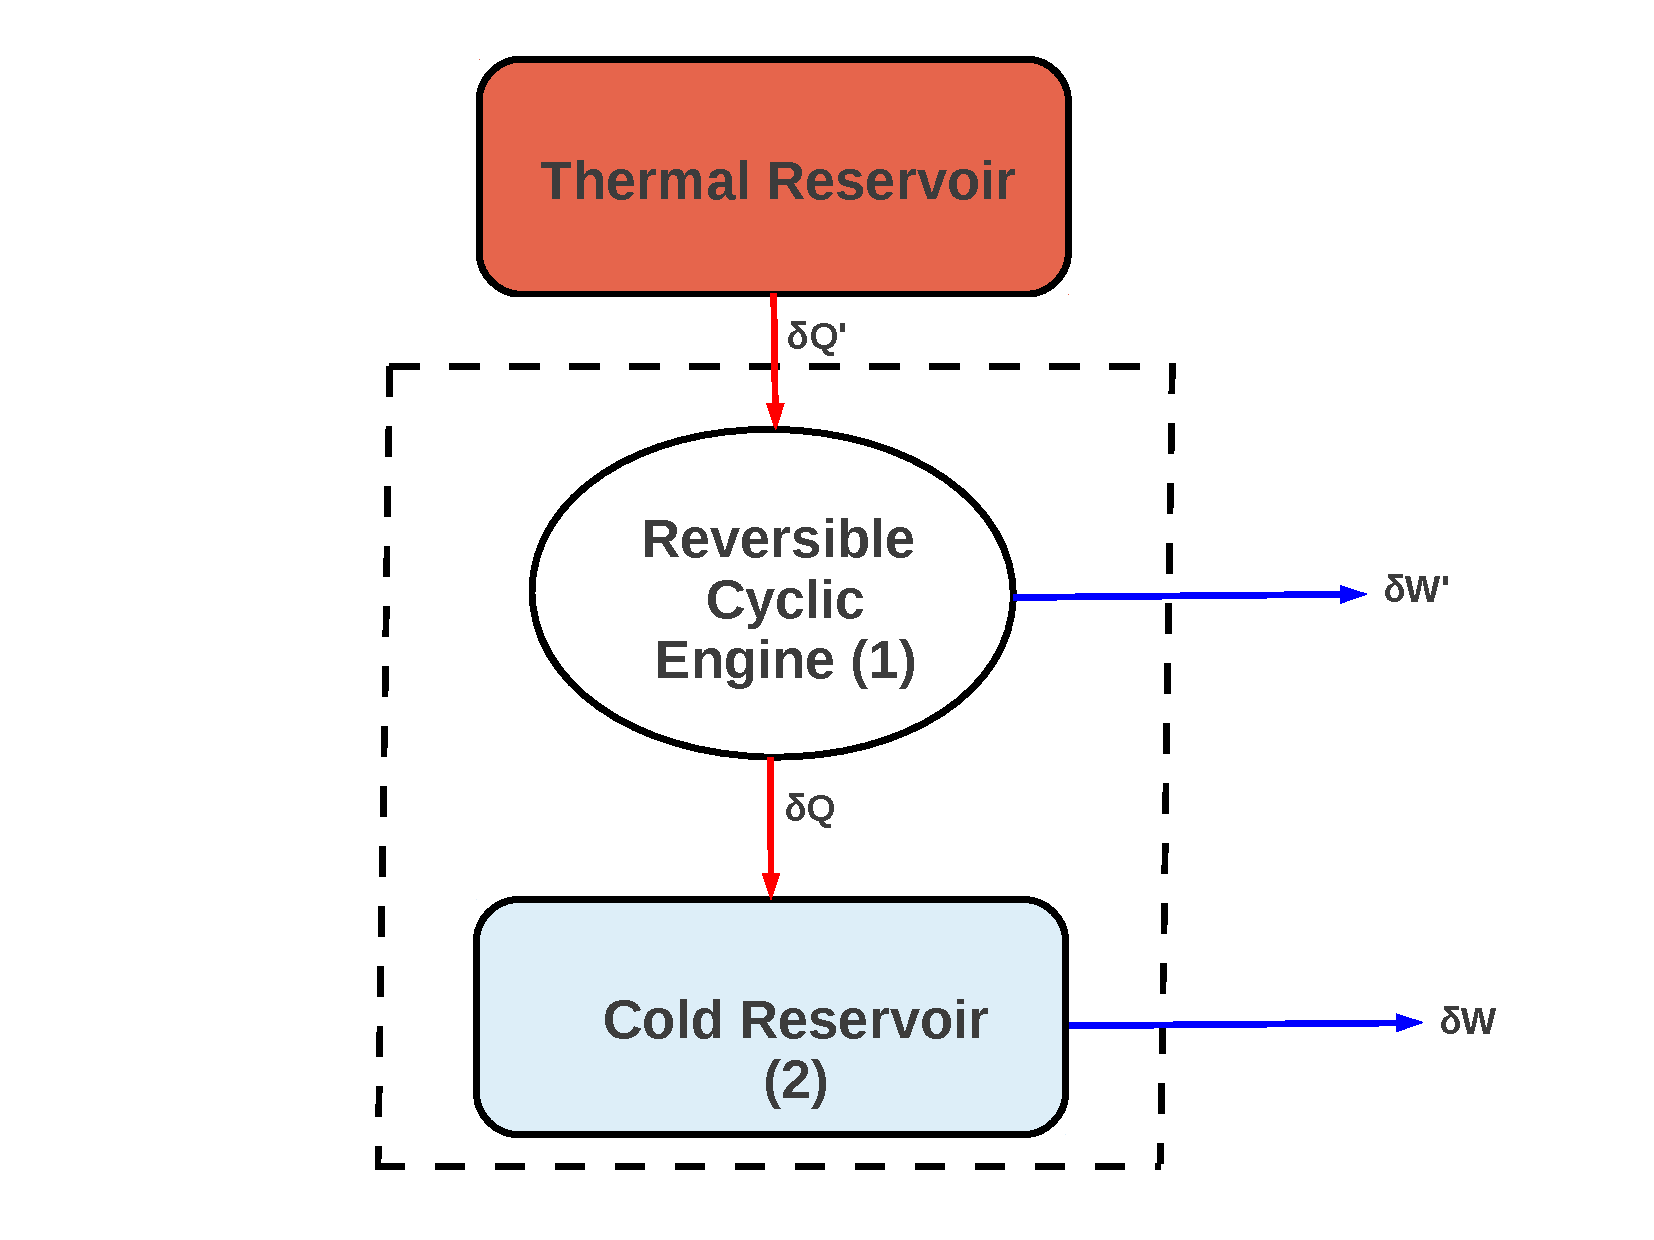
\includegraphics[width=1.1\columnwidth,clip]{./Pics/2ndLaw_Schem2}
    \end{center}
   \end{figure} 
  \end{column}
 \end{columns}


 \normalsize
    
\end{frame}


%%%
%%% Slides
%%%
\begin{frame}
 \frametitle{Derivation of the Mathematical Statement of the Second Law}
 %\scriptsize
 \begin{columns}

  \begin{column}[c]{0.5\linewidth}
   \begin{itemize}
    \item <1-> And eliminating $\delta Q^{\prime}$, \\
                $\delta W + \delta W^{\prime} = T_{res}\displaystyle\frac{\delta Q}{T} - dU$
     \item <2-> If the configuration shown in the previous slide undergoes a cyclic process, \\
             $\displaystyle\oint \delta W + \displaystyle\oint \delta W^{\prime} = \displaystyle\oint T_{res}\displaystyle\frac{\delta Q}{T} - \displaystyle\oint dU$
     \item <3-> as $U$ is a thermodynamic property, the cyclic integral is equal to zero.  Integrating the equation above, and assuming that $T_{res}$ is (by definition) constant:\\
             $W + W^{\prime} = T_{res} \displaystyle\oint \displaystyle\frac{\delta Q}{T}$
   \end{itemize}
  \end{column}

  \begin{column}[c]{0.5\linewidth}
   \begin{figure}%
    \begin{center}
     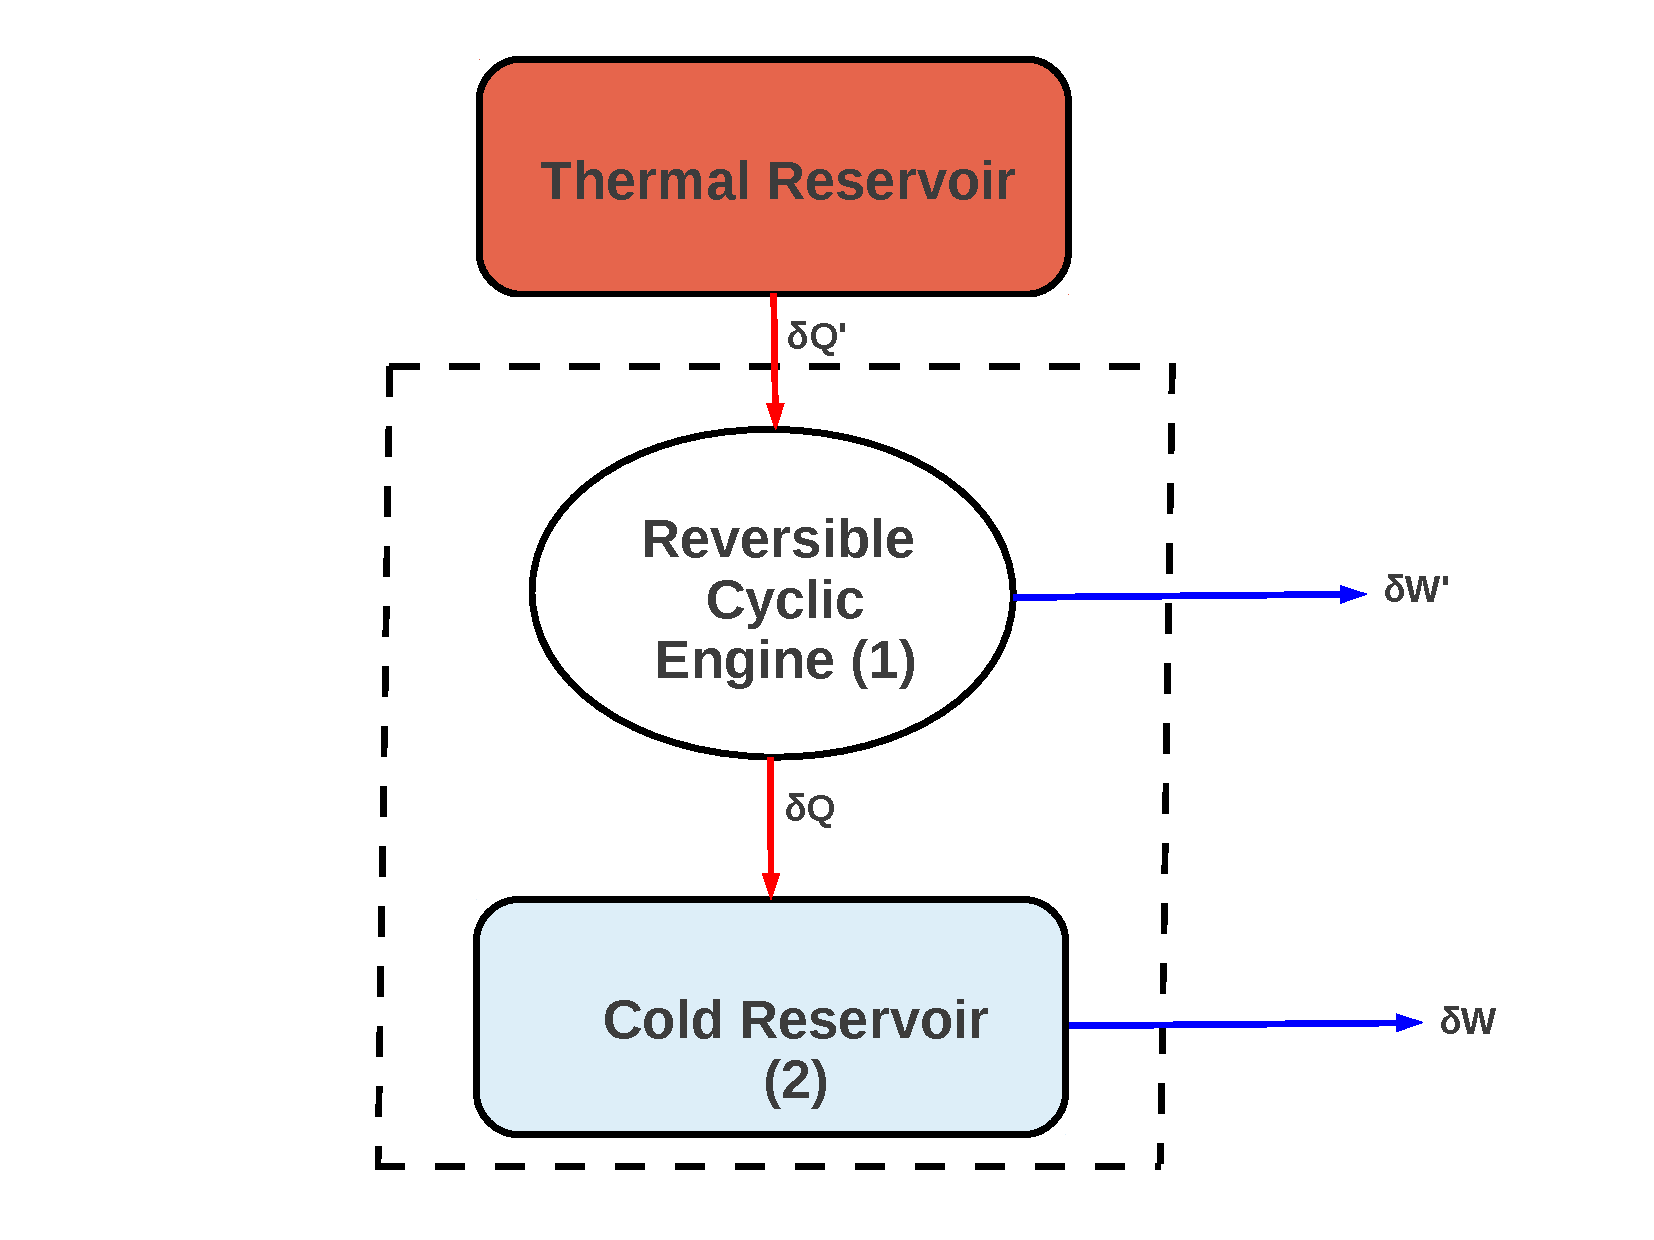
\includegraphics[width=1.1\columnwidth,clip]{./Pics/2ndLaw_Schem2}
    \end{center}
   \end{figure} 
  \end{column}
 \end{columns}
 \normalsize
    
\end{frame}


%%%
%%% Slides
%%%
\begin{frame}
 \frametitle{Derivation of the Mathematical Statement of the Second Law}
   \begin{itemize}
    \item <1-> Thus from Kelvin-Plancks statement of the Second Law -- \textcolor{blue}{$\lq$we cannot convert all the heat to work, but we can convert all the work to heat'}:\\
             $W + W^{\prime} \leq 0$
    \item <2-> And therefore,\\
             $T_{res} \displaystyle\displaystyle\oint \displaystyle\frac{\delta Q}{T} \leq 0$
    \item <3->  Since $T_{res} > 0$, we can divide the previous equation without changing the meaning of the inequality to obtain the mathematical representation of the Second Law:
             \begin{eqnarray}
             \textcolor{blue}{\displaystyle\oint \displaystyle\frac{\delta Q}{T} < 0 \;\;\; \text{for irreversible processes}} \nonumber \\
             \textcolor{blue}{\displaystyle\oint \displaystyle\frac{\delta Q}{T} = 0 \;\;\;\;\; \text{for reversible processes}} \nonumber 
             \end{eqnarray}
   \end{itemize}
 \normalsize
\end{frame}


%%%
%%% Slides
%%%
\begin{frame}
 \frametitle{Derivation of the Mathematical Statement of the Second Law}
   \begin{itemize}
    \item <1-> In a reversible process, from state 1 to 2, via path {\it A}, and returning to state 2 from either path {\it B} or {\it C}. The cyclic integral $\displaystyle\oint\displaystyle\frac{\delta Q}{T} = 0$ can be split as,
         \textcolor{blue}{\begin{eqnarray}
          \left( \displaystyle\int\limits_{1}^{2} \displaystyle\frac{\delta Q}{T} \right)_{A} + \left( \displaystyle\int\limits_{2}^{1} \displaystyle\frac{\delta Q}{T} \right)_{B} = 0 \nonumber \\
          \left( \displaystyle\int\limits_{1}^{2} \displaystyle\frac{\delta Q}{T} \right)_{A} + \left( \displaystyle\int\limits_{2}^{1} \displaystyle\frac{\delta Q}{T} \right)_{C} = 0 \nonumber 
         \end{eqnarray}}
   \end{itemize}
 \normalsize
    
\end{frame}

%%%
%%% Slides
%%%
\begin{frame}
 \frametitle{Derivation of the Mathematical Statement of the Second Law}
   \begin{itemize}
    \item <2-> Leading to:
          $\left( \displaystyle\int\limits_{1}^{2} \displaystyle\frac{\delta Q}{T} \right)_{B} = \left( \displaystyle\int\limits_{2}^{1} \displaystyle\frac{\delta Q}{T} \right)_{C} $
    \item <3-> Since paths {\it B} and {\it C} are different and arbitrary, but $\displaystyle\int\limits_{1}^{2}\displaystyle\frac{\delta Q}{T}$ is the same on either paths -- therefore \textcolor{blue}{the integral is path-independent};
    \item <4-> This defines another (extensive) thermodynamic property -- \textcolor{red}{entropy (S)}, \\
          $S_{2} - S_{1} = \displaystyle\int\limits_{1}^{2}\displaystyle\frac{\delta Q}{T}$
    \item <5-> Assuming constant mass ($m$), the intensive property entropy $\left(s=S/m\right)$, the differential form is, \\
          $ds = \displaystyle\frac{\delta q}{T} \;\;\;\; \Longrightarrow \;\;\;\; \delta q = Tds$
    \item <6-> Integrating from state 1 to 2: $q_{1}^{2} = \displaystyle\int_{1}^{2} Tds$    
   \end{itemize}
 \normalsize
\end{frame}


%%%
%%% Slides
%%%
\begin{frame}
 \frametitle{Derivation of the Mathematical Statement of the Second Law}
   \begin{itemize}
  \item <1-> This is the heat transfer equivalent of $w_{1}^{2}=\displaystyle\int_{1}^{2}PdV$
  \item <2-> Thus for a reversible process, \\
       $S_{2} - S_{1} = \displaystyle\int\limits_{1}^{2}\displaystyle\frac{\delta Q}{T}$ and $S_{1} - S_{2} = \displaystyle\int\limits_{2}^{1}\displaystyle\frac{\delta Q}{T}$;
  \item <3-> From the Second Law, \\
       $0 \geq \left( \displaystyle\int\limits_{1}^{2}\displaystyle\frac{\delta Q}{T} \right)_{A} + \left( \displaystyle\int\limits_{2}^{1}\displaystyle\frac{\delta Q}{T} \right)_{B}$ 
  \item <4-> Combinig the equations above to eliminate the path {\it B}, \\
        $S_{2}-S_{1} \geq \displaystyle\int\limits_{1}^{2}\displaystyle\frac{\delta Q}{T}$
 \end{itemize}
 \normalsize
\end{frame}


%%%
%%% Slides
%%%
\begin{frame}
 \frametitle{Derivation of the Mathematical Statement of the Second Law}
   \begin{itemize}
  \item <1-> If path {\it A} is reversible, the equality holds, however if {\it A} is irreversible, the inequality holds;
  \item <2-> If the system is isolated $\left(\delta Q = 0\right)$ then\\
    $S_{2}-S_{1}\geq 0$
   \end{itemize}
 \normalsize
    
\end{frame}


%%%
%%% SUBSECTION
%%%
\subsection{Entropy} 

%%%
%%% Slides
%%%
\begin{frame}
 \frametitle{Ideal Gas}
   \begin{enumerate}
     \item<1-> Mechanically reversible process of closed system
        \visible<1->{\begin{displaymath}
           dU = dQ_{\text{rev}} - PdV
        \end{displaymath}}
     \item<2-> Applying the definition of entropy and enthalpy,
        \visible<2->{\begin{displaymath}
           \displaystyle\frac{\Delta S}{R} = \int\limits_{T_{0}}^{T}\displaystyle\frac{C_{p}^{\text{ig}}}{R}\displaystyle\frac{d T}{T} - \ln\displaystyle\frac{P}{P_{0}}
        \end{displaymath}}
     \item<2-> This relates {\bf only} to \textcolor{blue}{properties}, i.e., \textcolor{blue}{independent of the process}.
   \end{enumerate}
 \normalsize
\end{frame}



\section{Summary}
%%%
%%% Slides
%%%
\begin{frame}
 \frametitle{Summary}
After these set of lectures you should know the fundamentals of thermodynamics which will be relevant to understand heat-engine and refrigeration cycles. This includes knowledge of: 
 \begin{itemize}
  \item <2-> Phase diagram and steam tables;
  \item <3-> Zeroth, First and Second Laws;
  \item <4-> Reversibility and its impact on thermodynamics formulation;
  \item <5-> Definition of the key thermodynamic properties, e.g., work, heat, temperature, internal energy, enthalpy, entropy, etc;
  \item <6-> Mass and energy balances in open and closed systems.
 \end{itemize}
\end{frame}

 
%%%
%%% Appendix
%%%
%\subsection{Appendix}
%\begin{frame}
%\begin{itemize}
%\item Saturated Water and Steam Tables;
%\item Superheated Steam at Various Pressure and Temperatures;
%\item Units Conversion.
%\end{itemize}
%\end{frame}


%{
%  
\includepdf[pages=-,fitpaper]{./Pics/Roschke.pdf}
%}


\end{document}
 % Introduction and Review of Thermodynamics

\part{Thermodynamic Properties of Fluids}
% Aberdeen style guide should be followed when using this
% layout. Their template powerpoint slide is used to extract the
% Aberdeen color and logo but is otherwise ignored (it has little or
% no formatting in it anyway).
%
% http://www.abdn.ac.uk/documents/style-guide.pdf

%%%%%%%%%%%%%%%%%%%% Document Class Settings %%%%%%%%%%%%%%%%%%%%%%%%%
% Pick if you want slides, or draft slides (no animations)
%%%%%%%%%%%%%%%%%%%%%%%%%%%%%%%%%%%%%%%%%%%%%%%%%%%%%%%%%%%%%%%%%%%%%%
%Normal document mode%
\documentclass[10pt,compress]{beamer}
%Draft or handout mode
%\documentclass[10pt,compress,handout]{beamer}
%\documentclass[10pt,compress,handout,ignorenonframetext]{beamer}

%%%%%%%%%%%%%%%%%%%% General Document settings %%%%%%%%%%%%%%%%%%%%%%%
% These settings must be set for each presentation
%%%%%%%%%%%%%%%%%%%%%%%%%%%%%%%%%%%%%%%%%%%%%%%%%%%%%%%%%%%%%%%%%%%%%%
\newcommand{\shortname}{jefferson.gomes@abdn.ac.uk}
\newcommand{\fullname}{Dr Jeff Gomes}
\institute{School of Engineering}
\newcommand{\emailaddress}{}%jefferson.gomes@abdn.ac.uk}
\newcommand{\logoimage}{../../FigBanner/UoAHorizBanner}
\title{Chemical Thermodynamics (EX3029)}
\subtitle{Module 2: Volumetric Properties of Pure Fluids}
\date[ ]{ }

%%%%%%%%%%%%%%%%%%%% Template settings %%%%%%%%%%%%%%%%%%%%%%%%%%%%%%%
% You shouldn't have to change below this line, unless you want to.
%%%%%%%%%%%%%%%%%%%%%%%%%%%%%%%%%%%%%%%%%%%%%%%%%%%%%%%%%%%%%%%%%%%%%%
\usecolortheme{whale}
\useoutertheme{infolines}

% Use the fading effect for items that are covered on the current
% slide.
\beamertemplatetransparentcovered

% We abuse the author command to place all of the slide information on
% the title page.
\author[\shortname]{%
  \fullname\\\ttfamily{\emailaddress}
}


%At the start of every section, put a slide indicating the contents of the current section.
\AtBeginSection[] {
  \begin{frame}
    \frametitle{Section Outline}
    \tableofcontents[currentsection]
  \end{frame}
}

% Allow the inclusion of movies into the Presentation! At present,
% only the Okular program is capable of playing the movies *IN* the
% presentation.
\usepackage{multimedia}
\usepackage{animate}

%% Handsout -- comment out the lines below to create handstout with 4 slides in a page with space for comments
\usepackage{handoutWithNotes}
%\pgfpagesuselayout{2 on 1 with notes}[a4paper,border shrink=10mm]
%%%%% Color settings
\usepackage{color}
%% The background color for code listings (i.e. example programs)
\definecolor{lbcolor}{rgb}{0.9,0.9,0.9}%
\definecolor{UoARed}{rgb}{0.64706, 0.0, 0.12941}
\definecolor{UoALight}{rgb}{0.85, 0.85, 0.85}
\definecolor{UoALighter}{rgb}{0.92, 0.92, 0.92}
\setbeamercolor{structure}{fg=UoARed} % General background and higlight color
\setbeamercolor{frametitle}{bg=black} % General color
\setbeamercolor{frametitle right}{bg=black} % General color
\setbeamercolor{block body}{bg=UoALighter} % For blocks
\setbeamercolor{structure}{bg=UoALight} % For blocks
% Rounded boxes for blocks
\setbeamertemplate{blocks}[rounded]

%%%%% Font settings
% Aberdeen requires the use of Arial in slides. We can use the
% Helvetica font as its widely available like so
% \usepackage{helvet}
% \renewcommand{\familydefault}{\sfdefault}
% But beamer already uses a sans font, so we will stick with that.

% The size of the font used for the code listings.
\newcommand{\goodsize}{\fontsize{6}{7}\selectfont}

% Extra math packages, symbols and colors. If you're using Latex you
% must be using it for formatting the math!
\usepackage{amscd,amssymb} \usepackage{amsfonts}
\usepackage[mathscr]{eucal} \usepackage{mathrsfs}
\usepackage{latexsym} \usepackage{amsmath} \usepackage{bm}
\usepackage{amsthm} \usepackage{textcomp} \usepackage{eurosym}
% This package provides \cancel{a} and \cancelto{a}{b} to "cancel"
% expressions in math.
\usepackage{cancel}

\usepackage{comment} 

%% Handsout -- comment out the lines below to create handstout with 4 slides in a page with space for comments
\usepackage{handoutWithNotes}

\mode<handout>
{
\usepackage{pgf,pgfpages}

\pgfpagesdeclarelayout{2 on 1 boxed with notes}
{
\edef\pgfpageoptionheight{\the\paperheight} 
\edef\pgfpageoptionwidth{\the\paperwidth}
\edef\pgfpageoptionborder{0pt}
}
{
\setkeys{pgfpagesuselayoutoption}{landscape}
\pgfpagesphysicalpageoptions
    {%
        logical pages=4,%
        physical height=\pgfpageoptionheight,%
        physical width=\pgfpageoptionwidth,%
        last logical shipout=2%
    } 
\pgfpageslogicalpageoptions{1}
    {%
    border code=\pgfsetlinewidth{1pt}\pgfstroke,%
    scale=1,
    center=\pgfpoint{.25\pgfphysicalwidth}{.75\pgfphysicalheight}%
    }%
\pgfpageslogicalpageoptions{2}
    {%
    border code=\pgfsetlinewidth{1pt}\pgfstroke,%
    scale=1,
    center=\pgfpoint{.25\pgfphysicalwidth}{.25\pgfphysicalheight}%
    }%
\pgfpageslogicalpageoptions{3}
    {%
    border shrink=\pgfpageoptionborder,%
    resized width=.7\pgfphysicalwidth,%
    resized height=.5\pgfphysicalheight,%
    center=\pgfpoint{.75\pgfphysicalwidth}{.29\pgfphysicalheight},%
    copy from=3
    }%
\pgfpageslogicalpageoptions{4}
    {%
    border shrink=\pgfpageoptionborder,%
    resized width=.7\pgfphysicalwidth,%
    resized height=.5\pgfphysicalheight,%
    center=\pgfpoint{.75\pgfphysicalwidth}{.79\pgfphysicalheight},%
    copy from=4
    }%

\AtBeginDocument
    {
    \newbox\notesbox
    \setbox\notesbox=\vbox
        {
            \hsize=\paperwidth
            \vskip-1in\hskip-1in\vbox
            {
                \vskip1cm
                Notes\vskip1cm
                        \hrule width\paperwidth\vskip1cm
                    \hrule width\paperwidth\vskip1cm
                        \hrule width\paperwidth\vskip1cm
                    \hrule width\paperwidth\vskip1cm
                        \hrule width\paperwidth\vskip1cm
                    \hrule width\paperwidth\vskip1cm
                    \hrule width\paperwidth\vskip1cm
                    \hrule width\paperwidth\vskip1cm
                        \hrule width\paperwidth
            }
        }
        \pgfpagesshipoutlogicalpage{3}\copy\notesbox
        \pgfpagesshipoutlogicalpage{4}\copy\notesbox
    }
}
}

%\pgfpagesuselayout{2 on 1 boxed with notes}[letterpaper,border shrink=5mm]
%\pgfpagesuselayout{2 on 1 boxed with notes}[letterpaper,border shrink=5mm]


% Get rid of font warnings as modern LaTaX installations have scalable
% fonts
\usepackage{type1cm} 

%\usepackage{enumitem} % continuous numbering throughout enumerate commands

% For exact placement of images/text on the cover page
\usepackage[absolute]{textpos}
\setlength{\TPHorizModule}{1mm}%sets the textpos unit
\setlength{\TPVertModule}{\TPHorizModule} 

% Source code formatting package
\usepackage{listings}%
\lstset{ backgroundcolor=\color{lbcolor}, tabsize=4,
  numberstyle=\tiny, rulecolor=, language=C++, basicstyle=\goodsize,
  upquote=true, aboveskip={1.5\baselineskip}, columns=fixed,
  showstringspaces=false, extendedchars=true, breaklines=false,
  prebreak = \raisebox{0ex}[0ex][0ex]{\ensuremath{\hookleftarrow}},
  frame=single, showtabs=false, showspaces=false,
  showstringspaces=false, identifierstyle=\ttfamily,
  keywordstyle=\color[rgb]{0,0,1},
  commentstyle=\color[rgb]{0.133,0.545,0.133},
  stringstyle=\color[rgb]{0.627,0.126,0.941}}

% Allows the inclusion of other PDF's into the final PDF. Great for
% attaching tutorial sheets etc.
\usepackage{pdfpages}
\setbeamercolor{background canvas}{bg=}  

% Remove foot note horizontal rules, they occupy too much space on the slide
\renewcommand{\footnoterule}{}

% Force the driver to fix the colors on PDF's which include mixed
% colorspaces and transparency.
\pdfpageattr {/Group << /S /Transparency /I true /CS /DeviceRGB>>}

% Include a graphics, reserve space for it but
% show it on the next frame.
% Parameters:
% #1 Which slide you want it on
% #2 Previous slides
% #3 Options to \includegraphics (optional)
% #4 Name of graphic
\newcommand{\reserveandshow}[4]{%
\phantom{\includegraphics<#2|handout:0>[#3]{#4}}%
\includegraphics<#1>[#3]{#4}%
}

\newcommand{\frc}{\displaystyle\frac}
\newcommand{\red}{\textcolor{red}}
\newcommand{\blue}{\textcolor{blue}}
\newcommand{\green}{\textcolor{green}}
\newcommand{\purple}{\textcolor{purple}}
 
\begin{document}

% Title page layout
\begin{frame}
  \titlepage
  \vfill%
  \begin{center}
    \includegraphics[clip,width=0.8\textwidth]{\logoimage}
  \end{center}
\end{frame}

% Table of contents
\frame{ \frametitle{Slides Outline}
  \tableofcontents
}


%%%%%%%%%%%%%%%%%%%% The Presentation Proper %%%%%%%%%%%%%%%%%%%%%%%%%
% Fill below this line with \begin{frame} commands! It's best to
% always add the fragile option incase you're going to use the
% verbatim environment.
%%%%%%%%%%%%%%%%%%%%%%%%%%%%%%%%%%%%%%%%%%%%%%%%%%%%%%%%%%%%%%%%%%%%%%


%%%
%%% SECTION
%%%
\section{General Remarks}

%%%
%%% Slides
%%%
\begin{frame}
 \frametitle{Aims and Objectives}
   \begin{enumerate}
     \item<1-> In Module 1, we learnt:
       \begin{enumerate}
         \item<1-> the laws of Thermodynamics and how they describe thermal equilibrium of species in closed and open systems.
         \item<1-> how to obtain and calculate relevant thermodynamics properties for chemical species.
         \item<1-> reversibility  of processes.
       \end{enumerate} 
     \item<2-> This Module focuses on 
         \begin{enumerate}
           \item<2-> PVT behaviour of pure chemical species in equilibrium,
           \item<2-> Equations of state commonly used in industry.
         \end{enumerate}
   \end{enumerate}

\end{frame}


%%%
%%% SECTION
%%%
\section{Bibliography}
\begin{frame}
 \frametitle{Suggested References}
  Literature relevant for this module:
  \begin{enumerate}[1.]
   \item J.M. Smith, H.C. Van Ness, M.M. Abbott, $\lq$Introduction to Chemical Engineering Thermodynamics', 6$^{th}$ Edition: Chapter 3;
   \item Y.A. Cengel, M.A. Boles, $\lq$Thermodynamics -- An Engineering Approach', 5$^{th}$ Edition: Chapter 3; 
   \item M.J. Moran, H.N. Saphiro, D.D. Boettner, M.B. Bailey, $\lq$Principles of Engineering Thermodynamics', 7$^{th}$ Edition: Chapters 3;
   \item C. Borgnakke, R.E. Sonntag, $\lq$Fundamentals of Thermodynamics', 8$^{th}$ Edition: Chapter 2.
  \end{enumerate}
\end{frame}



%%%
%%% SECTION
%%%
\section{PVT Behaviour of Pure Substances}

%%%
%%% SUBSECTION
%%%
\subsection{Phase Diagram and Gibbs Rule} 

%%%
%%% Slide
%%%
\begin{frame}
 \frametitle{PVT Behaviour of Pure Substances}
 \begin{columns}
  \begin{column}[l]{0.5\linewidth}
    \begin{enumerate}\scriptsize
    \item <1-> This surface represents the \textcolor{red}{Pressure} - \textcolor{red}{specific volume} - \textcolor{red}{Temperature} -- $PVT$, relation in a pure substance;
    \item <2-> Any given coordinate in both, the surface plot and diagrams (projections), will represent values of pressure, specific volume and temperature when the substance is at equilibrium;
    \item <3-> The \textcolor{red}{Gibbs phase rule},
       \visible<3->{\begin{equation}
          \Psi = 2 + \mathcal{C} - \mathcal{P}
       \end{equation} 
       describes the number of degrees of freedom (dof), $\Psi$ (\underline{intensive variables}, e.g., temperature, pressure), in a closed system at equilibrium as a function of the number of phases ($\mathcal{P}$ = solid, liquid and/or vapour) and components, $\mathcal{C}$ (e.g., water, CO$_{2}$, N$_{2}$, etc). }
\end{enumerate}
  \end{column}
  \begin{column}[l]{0.5\linewidth}
   \begin{figure}%
    \begin{center}
     \includegraphics[width=4.cm,clip]{./../Pics/PVT_Surface.jpg}
    \end{center}
    \scriptsize\caption{\scriptsize$PVT$ volume (top) and projections onto (b) $PT$ and (c) $PV$ diagrams for a pure substance (Extracted from [4]).}
   \end{figure}    
  \end{column}
 \end{columns}
\end{frame}

%%%
%%% Slide
%%%
\begin{frame}
 \frametitle{PT Diagram}
 \begin{columns}
   \begin{column}[l]{0.5\linewidth}
     \begin{enumerate}\scriptsize
        \item<1-> The \textcolor{blue}{$PT$ phase diagram} describes fluid behaviour and phase change; 
        \item<2-> For example: \textcolor{blue}{A}-\;-\;-\textcolor{red}{B} defines a phase transition from \textcolor{blue}{liquid} to \textcolor{red}{gas} regions without crossing the phase boundary (vaporisation);
        \item <3-> {\bf Example 1:} In the $PT$ diagram for one hypothetical component -- $\textcolor{red}{\mathcal{C}=1}$, within each phase region -- $\textcolor{blue}{\mathcal{P}=1}$ (i.e., as either solid, liquid or vapour phase),
          \visible<3->{\begin{displaymath}
            \Psi = 2 + \textcolor{red}{1} - \textcolor{blue}{1} = 2
          \end{displaymath}
          \begin{enumerate}[(a)]\scriptsize
             \item  In this case, the number of degrees of freedom correspond to temperature and pressure;
             \item  Thus, within the vapour phase, temperature and pressure can readily be changed without explicit phase change or composition of the vapour phase.
          \end{enumerate}}
        \item <4-> {\bf Example 2:} However, along with the \textcolor{red}{phase-line boundary}, two phases are in equilibrium, i.e., $\textcolor{blue}{\mathcal{P}=2}$,%
          \visible<2->{\begin{displaymath}
            \Psi = 2 + \textcolor{red}{1} - \textcolor{blue}{2} = 1,
          \end{displaymath}}
     \end{enumerate}
  \end{column}
  \begin{column}[l]{0.5\linewidth}\scriptsize
          \visible<4->{when the vapour and liquid phases are in equilibrium, any change in temperature {\bf leads} to change in pressure for the system remains in equilibrium;}
      \begin{figure}%
        \begin{center}
          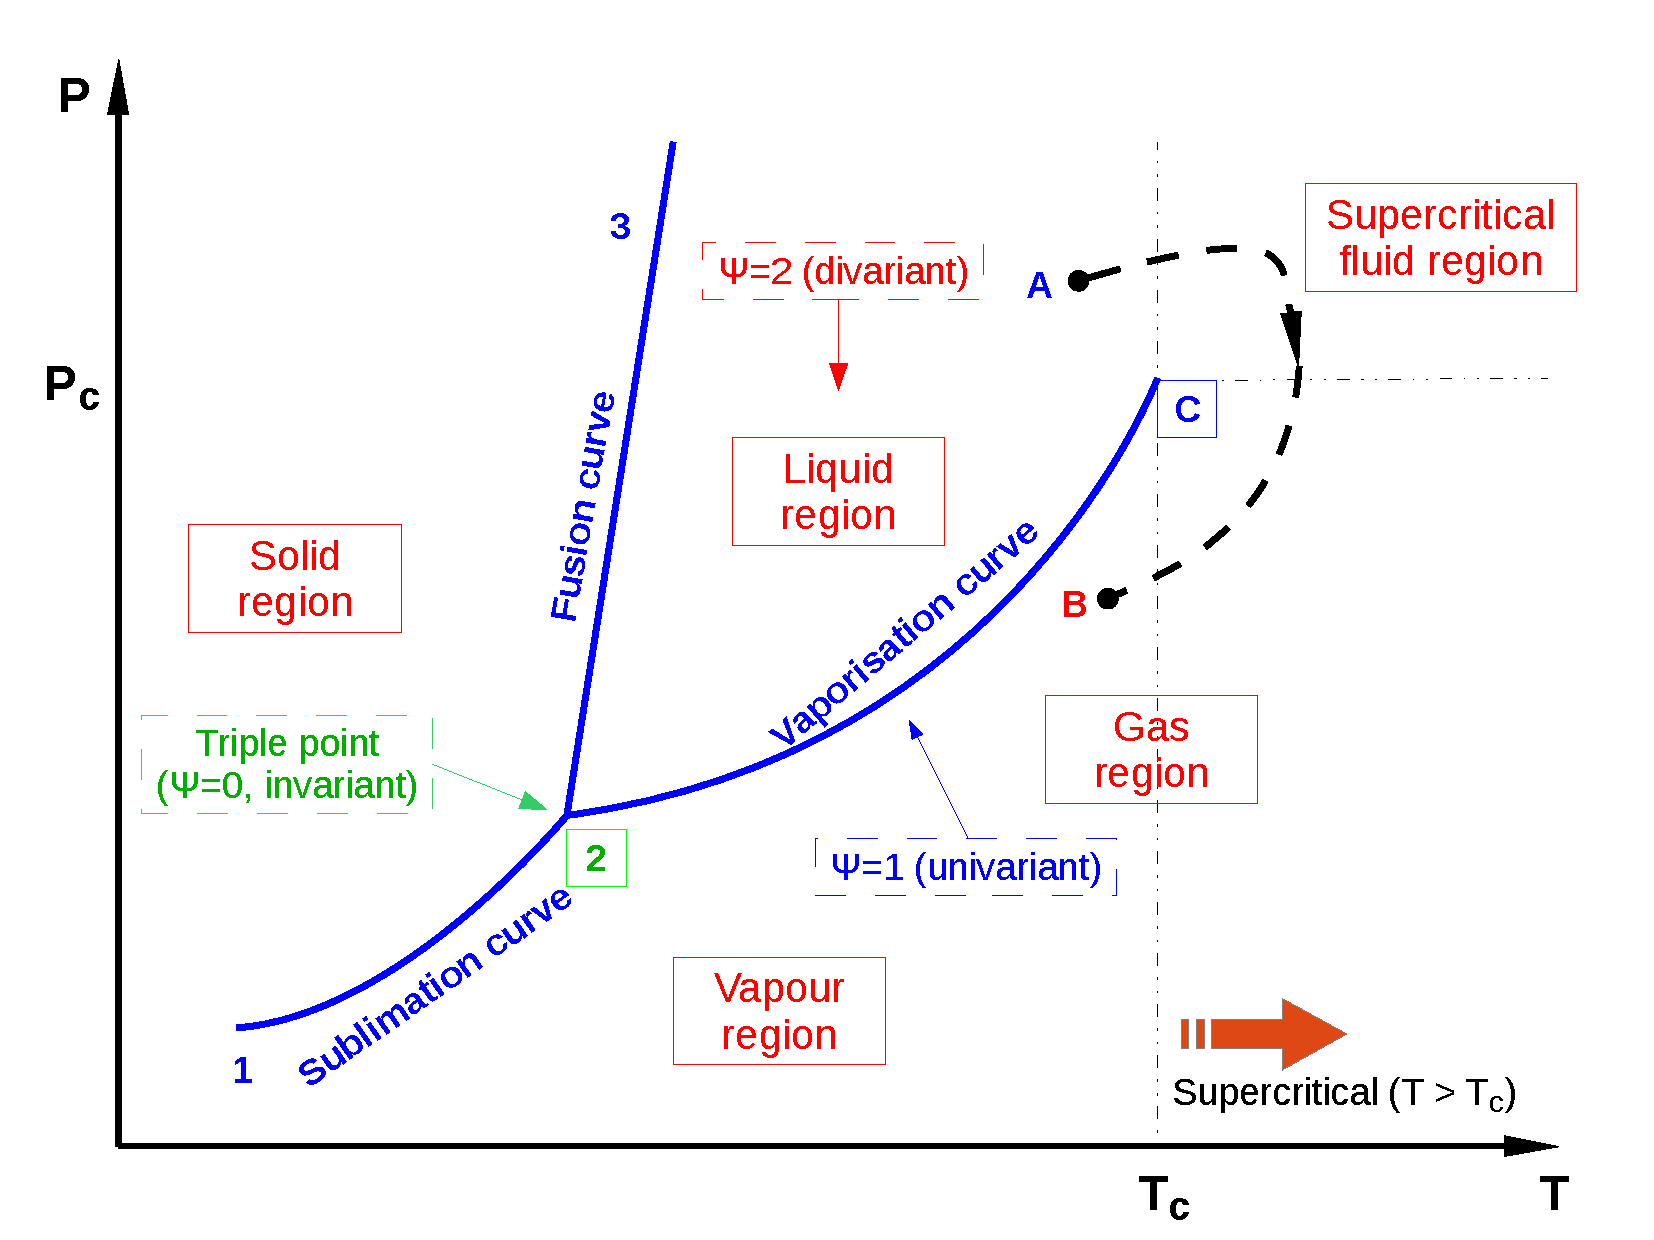
\includegraphics[width=1.05\columnwidth,clip]{./../Pics/PT_Diagram}
        \end{center}
      \end{figure}
     \begin{enumerate}\setcounter{enumi}{4}\scriptsize
        \item<5-> However, there is \red{no} information about the volume in the {\it PT} diagram.
     \end{enumerate}
  \end{column}
 \end{columns}
\end{frame}
 
%%%
%%% Slide
%%%
\scriptsize
\begin{frame}
 \frametitle{PV Diagram}
  \begin{columns}
    \begin{column}[l]{0.5\linewidth}
      \visible<1->{\begin{figure}%
        \begin{center}
          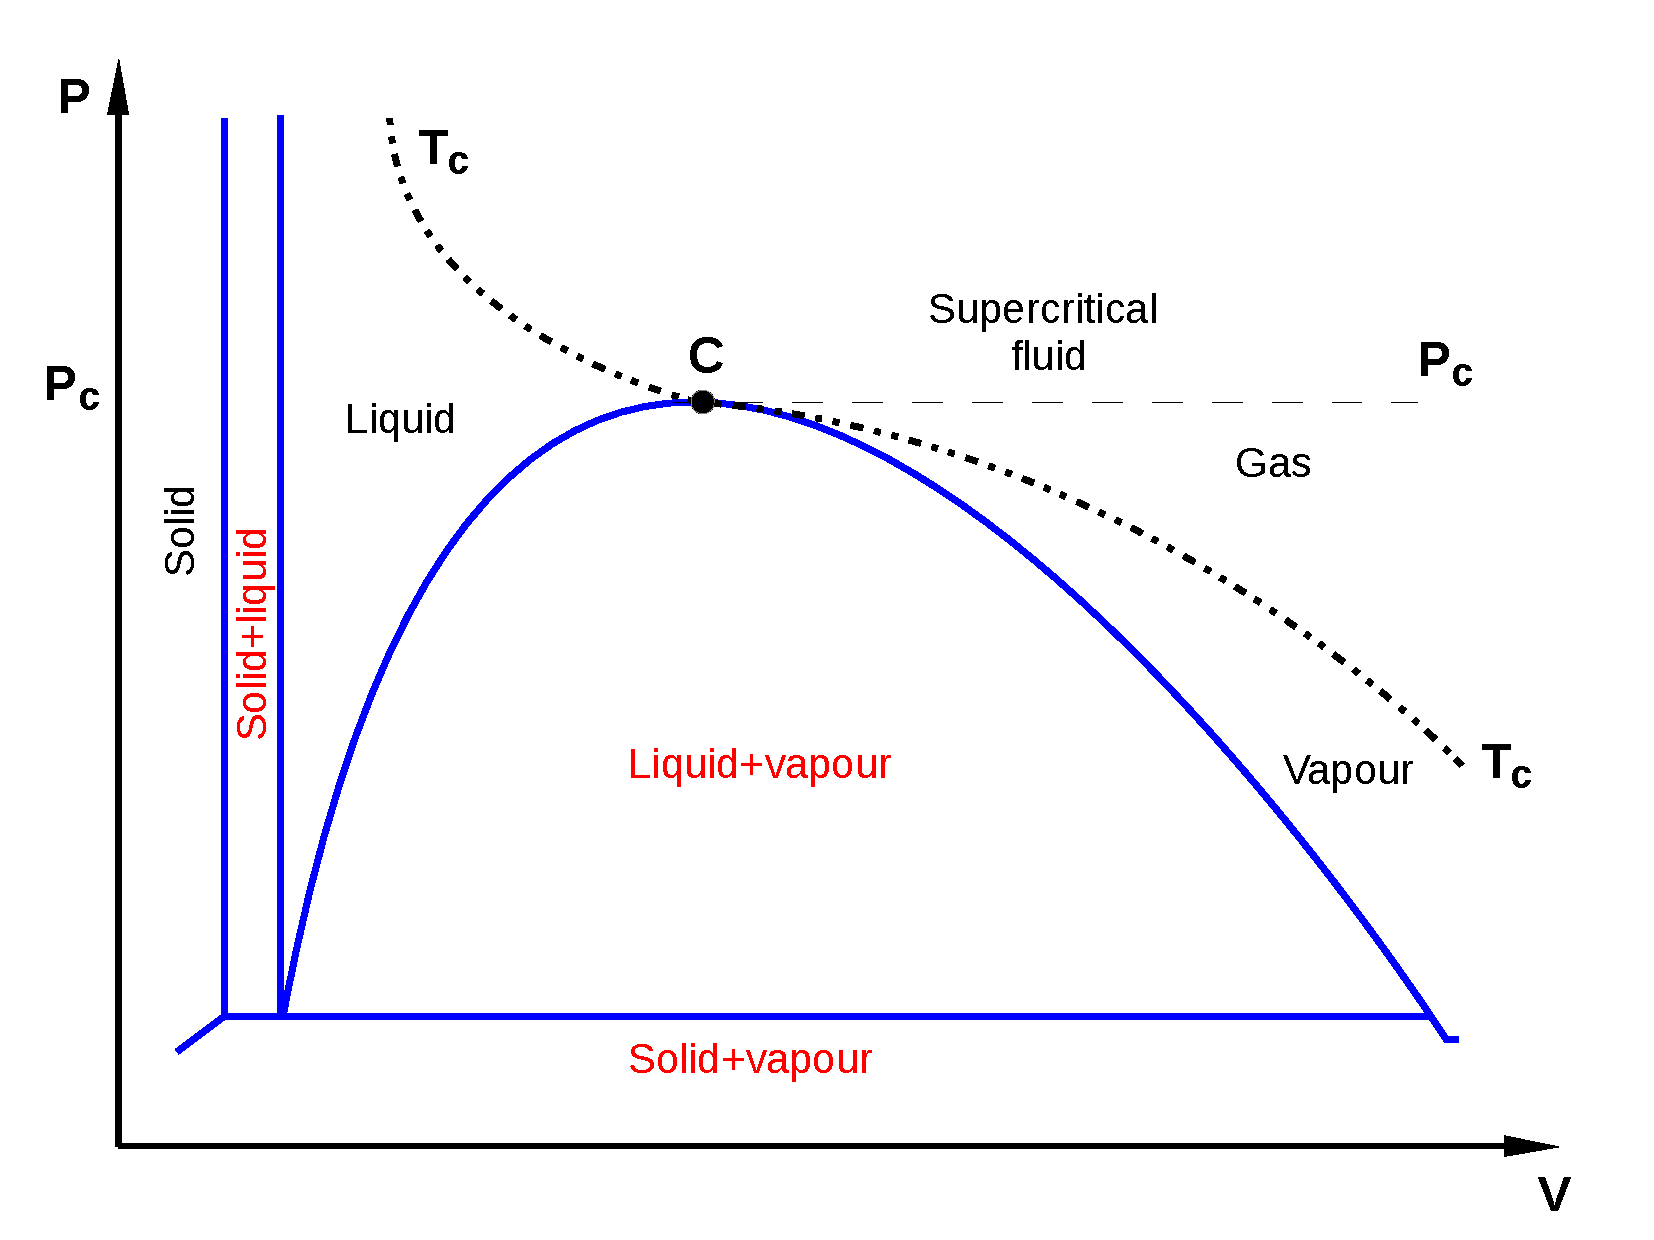
\includegraphics[width=\columnwidth,clip]{./../Pics/PV_Diagram1}
        \end{center}
      \end{figure}}
      \begin{enumerate} \scriptsize
        \item<1-> Two-phase regions (e.g., liquid+vapor) are represented by \textcolor{red}{areas} and;
        \item<2-> Lines represent the actual transition transition between \textcolor{blue}{single phase} to \textcolor{blue}{two phases} regions, thus;
        \item<2-> The \textcolor{blue}{triple point} is the horizontal line between the 3 phases;
      \end{enumerate}
    \end{column}
    \begin{column}[l]{0.5\linewidth}\scriptsize
      \visible<3->{\begin{figure}%
        \begin{center}
          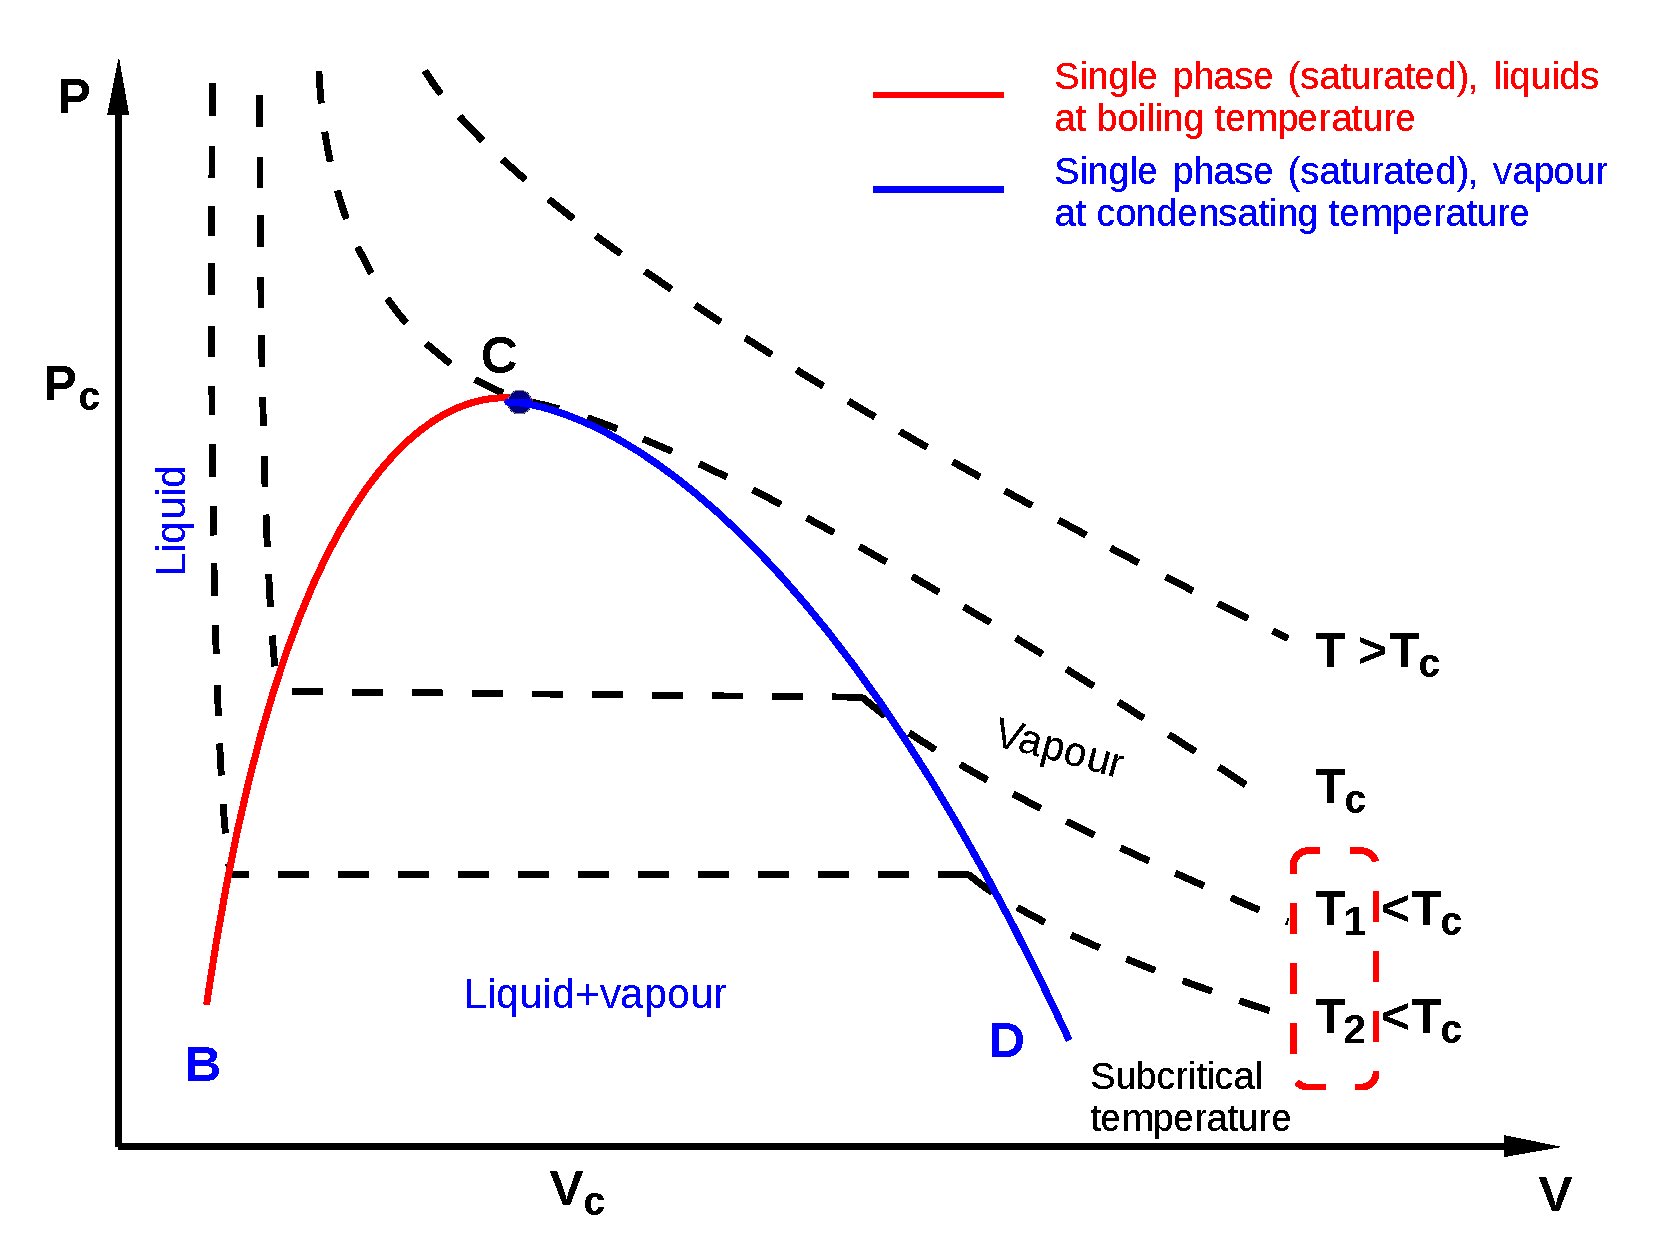
\includegraphics[width=\columnwidth,clip]{./../Pics/PV_Diagram2}
        \end{center}
      \end{figure}}
      \begin{enumerate}\setcounter{enumi}{3}
        \item<3-> The isotherms range from \textcolor{blue}{subcooled liquid} to \textcolor{blue}{superheated vapor} regions; 
        \item<3-> Isotherms are \textcolor{red}{steep} in the \textcolor{blue}{subcooled liquid}  region because liquid volumes have little changes with large change in pressure.
      \end{enumerate}
    \end{column}
  \end{columns}
\end{frame}
\normalsize

%%%% COMMENTS
\begin{comment}
%%%
%%% Slide
%%%
\scriptsize
\begin{frame}
 \frametitle{PV Diagram}
      \visible<1->{\begin{figure}%
        \begin{center}
          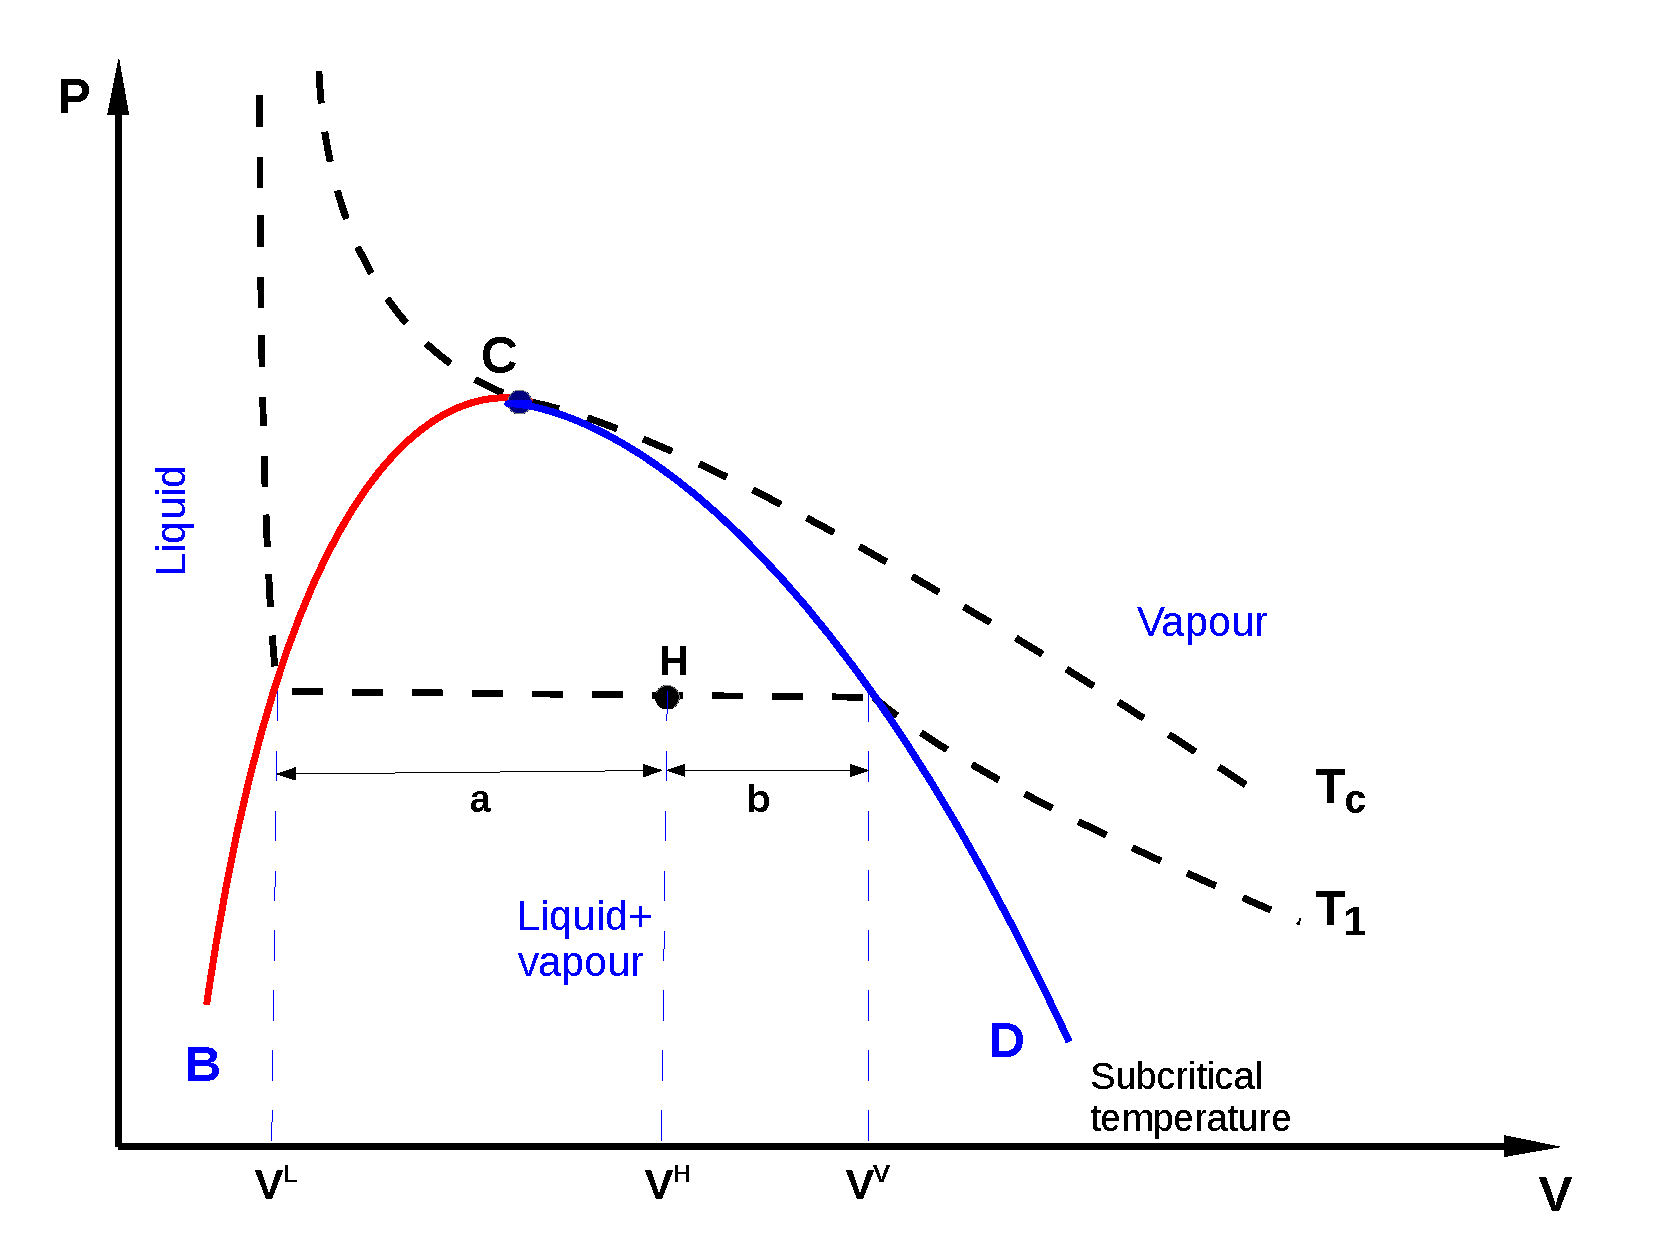
\includegraphics[width=.6\columnwidth,clip]{./../Pics/PV_Diagram3}
        \end{center}
      \end{figure}}
      \visible<2->{\begin{displaymath}
         \frc{a}{b} = \frc{V^{H}-V^{L}}{V^{V}-V^{H}} = \frc{m^{V}}{m^{L}} = \frc{\text{mass of saturated vapour}}{\text{mass of saturated liquid}}
      \end{displaymath}}
     
\end{frame}
\normalsize
\end{comment}

%%%
%%% Slide
%%%
\scriptsize
\begin{frame}
 \frametitle{Single Phase region}
    \begin{enumerate}\scriptsize
      \item<1-> \textcolor{blue}{Equations of State (EOS)} relates pressure, molar or specific volume and temperature of any \textcolor{blue}{pure homogeneous fluid} in equilibrium states;
      \item<2-> We can express it as a general functional,
          \visible<2->{\begin{displaymath}
              f\left(P, V, T\right) = 0
          \end{displaymath} 
          where $P$, $V$ or $T$ can be expressed as a function of two of this properties.}
      \item<3-> For example, we can represent the volume as $V=V\left(T,P\right)$, thus
          \visible<3->{\begin{equation}
              dV = \left(\frc{\partial V}{\partial T}\right)_{P} dT + \left(\frc{\partial V}{\partial P}\right)_{T} dP \;\;\Longrightarrow \;\; \textcolor{blue}{\frc{dV}{V} = \beta dT - \kappa dP} \label{genericV}
          \end{equation} 
            with $\beta  =  \frc{1}{V}\left(\frc{\partial V}{\partial T}\right)_{P}$ (coefficient of thermal expansion or volume expansivity coefficient) and $\kappa = -\frc{1}{V}\left(\frc{\partial V}{\partial P}\right)_{T}$ (coefficient of isothermal compressibility).
           }
      \item<4-> A few useful remarks:
        \begin{itemize}\scriptsize
          \item<4-> For \textcolor{blue}{incompressible fluids}: $\beta$ and $\kappa$ are zero;
          \item<4-> For liquids: $\beta>0$ (except for liquid H$_{2}$O at $0\leq T\leq 4^{\circ}$C) and $\kappa>0$  
        \end{itemize}
      \item<5-> Close to the critical point, $\beta$ and $\kappa$ are assumed constant, thus \blue{Eqn.~\ref{genericV}} becomes, 
        \visible<5->{\begin{displaymath}
            \ln\frc{V_{2}}{V_{1}} = \beta\left(T_{2}-T_{1}\right) - \kappa\left(P_{2}-P_{1}\right)
        \end{displaymath}}
    
    \end{enumerate}
\end{frame}
\normalsize

%%%
%%% SECTION
%%%
\section{Equations of State (EOS)}

%%%
%%% Slide
%%%
\scriptsize
\begin{frame}
 \frametitle{Summary List of EOS}
      \visible<1->{\begin{figure}%
        \begin{center}
          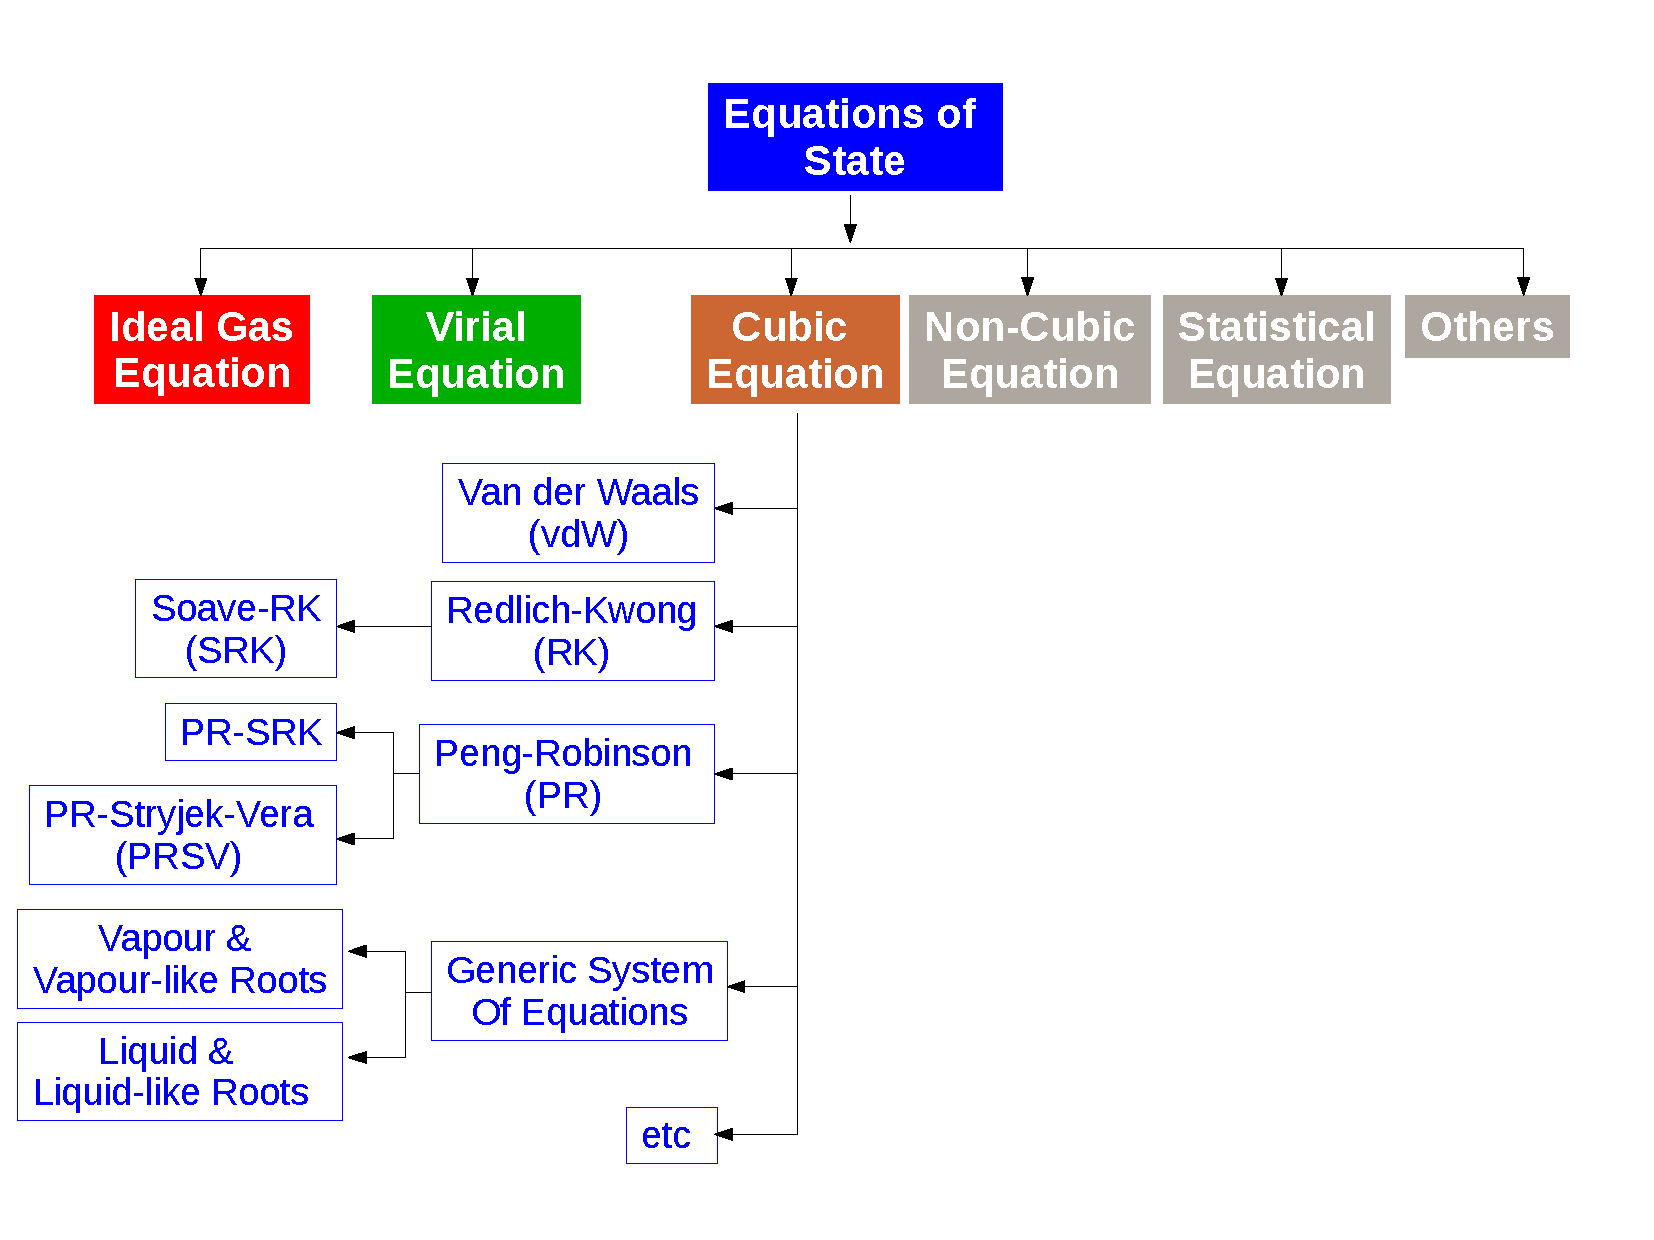
\includegraphics[width=0.9\columnwidth,clip]{./../Pics/ListEOS}
        \end{center}
      \end{figure}}
\end{frame}
\normalsize


%%%
%%% SUBSECTION
%%%
\subsection{Virial EOS}

%%%
%%% Slide
%%%
\scriptsize
\begin{frame}
 \frametitle{Virial Expansion}
   \begin{columns}
    \begin{column}[l]{0.5\linewidth}
      \begin{enumerate} \scriptsize
        \item<1-> $\left(PV\right)$ along an isotherm can be expressed as function of {\bf P} by a \textcolor{blue}{power series},
           \visible<1->{\begin{displaymath}
             \left(PV\right) = a + bP + cP^{2} + dP^{3} + \cdots
           \end{displaymath}}
        \item<2-> Defining $b=aB^{\prime}$, $c=aC^{\prime}$, $d=aD^{\prime}$, $\cdots$, then
           \visible<2->{\begin{equation}\label{Mod3:VirialEoS1}
             \left(PV\right) = a\left( 1 + B^{\prime}P + C^{\prime}P^{2} + D^{\prime}P^{3} + \cdots\right) 
           \end{equation}}
        \item<2-> $B^{\prime}$, $C^{\prime}$ and $D^{\prime}$ are constants, characteristic for each chemical species and temperature-dependent $\left(\text{i.e.,} B^{\prime}=B^{\prime}(T), C^{\prime}=C^{\prime}(T)\right)$  
        \item<3-> In the limit case -- $P\rightarrow 0$, \textcolor{blue}{$\left(PV\right)$ for all gases}:\\
           \begin{displaymath}
              \visible<3->{\textcolor{blue}{\left(PV\right)^{\star} =}} 
                   \begin{cases}
                      \visible<3->{a = f\left(T\right)} \\
                      \visible<4->{\textcolor{blue}{a= RT}}\\ 
                   \end{cases}
           \end{displaymath}
           \visible<4->{where $R$ is a proportionally constant, i.e.,  universal gas constant.}
        \item<5-> At this limiting case, $\left(PV\right)_{T}^{\star} = R \times 273.16$. 
      \end{enumerate}
    \end{column}
    \begin{column}[l]{0.5\linewidth}\scriptsize
     \begin{enumerate}\setcounter{enumi}{5}
       \item<6->For \textcolor{blue}{ideal gasses}, pressure is sufficiently small $\left(P\rightarrow 0\right)$. 
       \item<6-> This means that the molecules are separated by infinite distances, and therefore the \textcolor{blue}{intermolecular forces approaches zero}. 
     \end{enumerate}
      \visible<3->{\begin{figure}%
        \begin{center}
          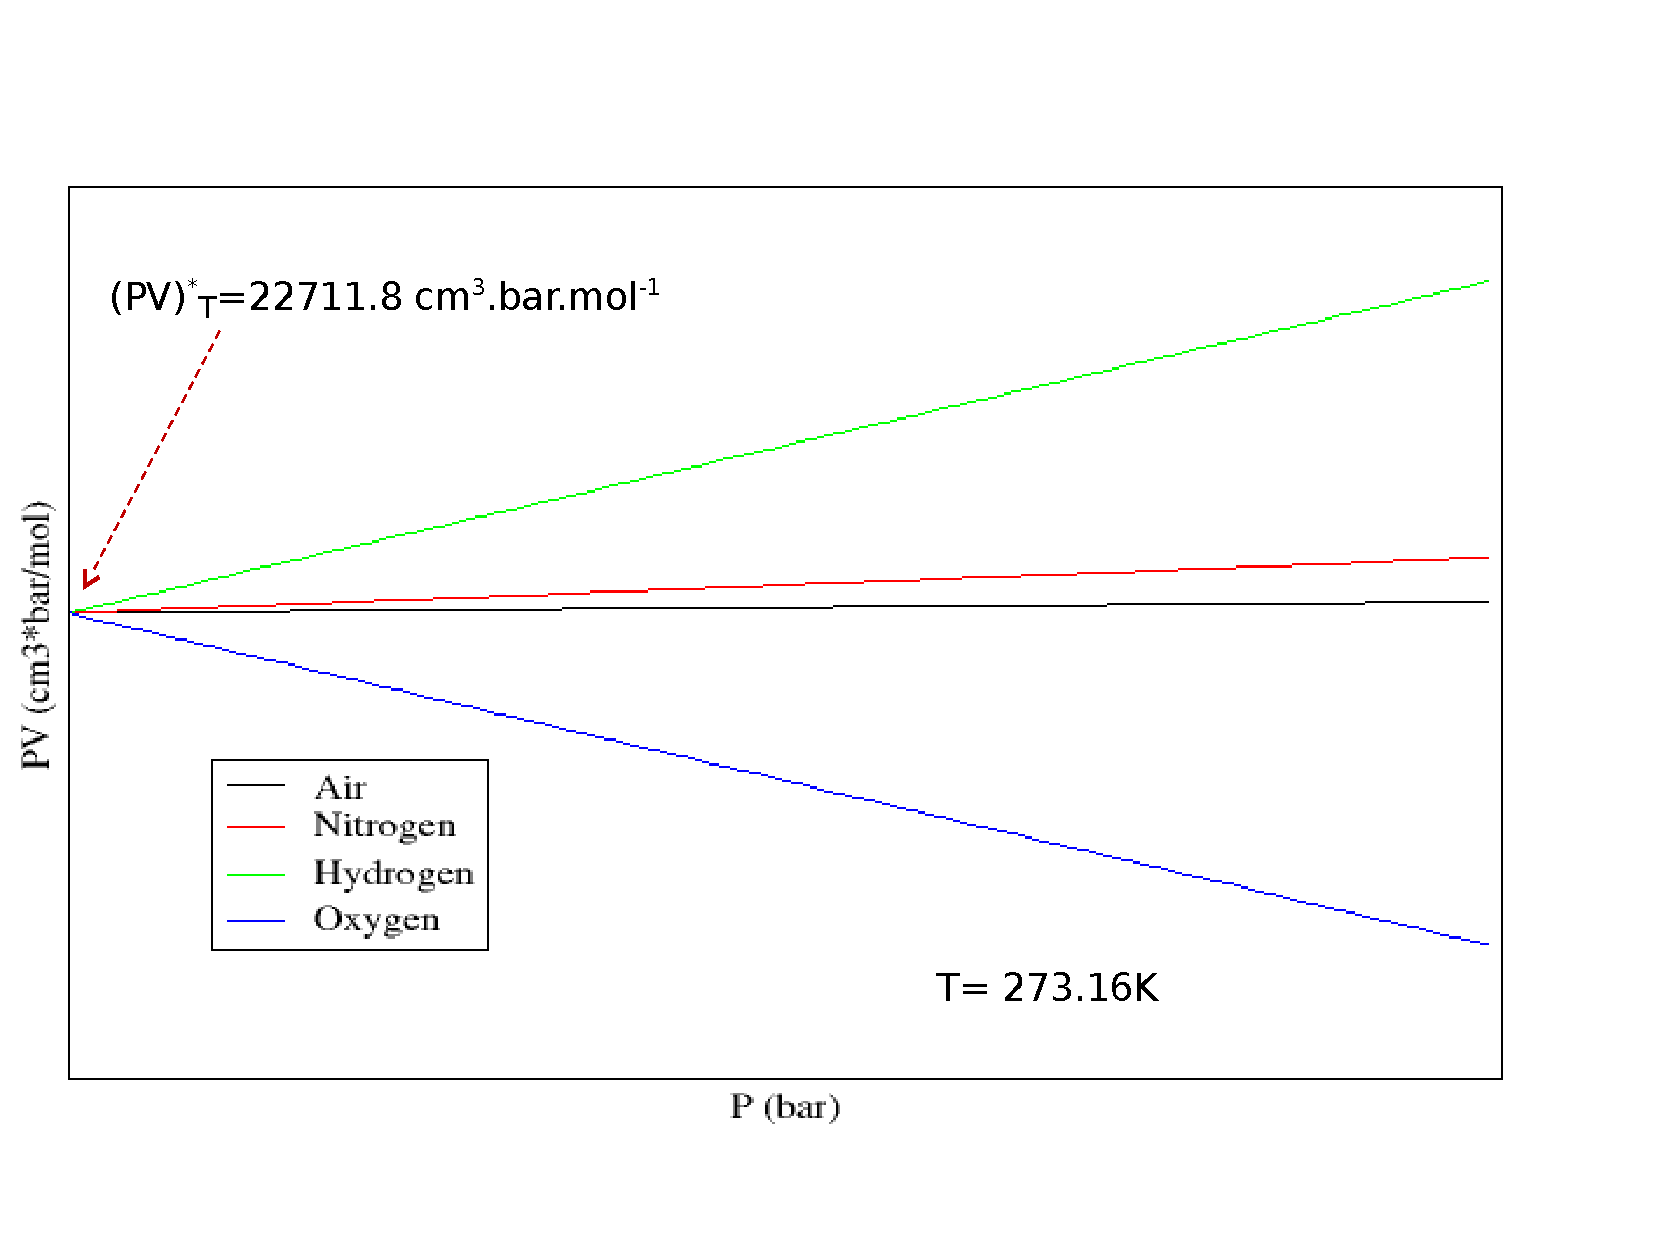
\includegraphics[width=1.05\columnwidth,clip]{./../Pics/Virial_EOS}
        \end{center}
      \end{figure}}
    \end{column}
  \end{columns}

\end{frame}
\normalsize


%%%
%%% Slide
%%%
\scriptsize
\begin{frame}
 \frametitle{Compressibility Factor -- $Z$}
   \begin{enumerate}\setcounter{enumi}{7}\scriptsize
     \item<1-> The {\it Virial expansion} is considered the only EOS based on rigorous mathematical derivation. It can also be derived from statistical mechanics leading to physical  significance of the virial coefficients;
     \item<2->The original form of the Virial EOS (Eqn.~\ref{Mod3:VirialEoS1}) can be rewritten as
        \begin{equation}\label{Mod3:VirialEoS2}
            \visible<2->{\frc{PV}{RT}} \visible<3->{ = \textcolor{red}{Z}} = \visible<2->{1 + B^{\prime}P + C^{\prime}P^{2} + D^{\prime}P^{3} + \cdots}
        \end{equation}
     \item<4-> \textcolor{red}{$Z$} is the \textcolor{blue}{compressibility factor} and is commonly used to estimate the deviation from ideal gas behaviour.
     \item<5->Therefore, the Virial EOS can be represented by 2 main forms:
        \begin{equation}
          Z = \frc{PV}{RT} =
             \begin{cases}
                1 + \textcolor{blue}{\frc{B}{V}} + \textcolor{red}{\frc{C}{V^{2}}} + \textcolor{purple}{\frc{D}{V^{3}}} + \cdots \\
                \visible<6->{1 + \blue{B^{\prime}P} + \red{C^{\prime}P^{2}} + \purple{D^{\prime}P^{3}} + \cdots} \\
                \visible<7->{1 + \blue{\frc{B}{RT}P} + \red{\frc{C-B^{2}}{\left(RT\right)^{2}}P^{2}} + \purple{\frc{D-3BC+2B^{2}}{\left(RT\right)^{3}}P^{3}} + \cdots}
             \end{cases}
        \end{equation}
     \item<8-> Thus, for real cases
        \begin{equation}
          \visible<8->{Z = \frc{PV}{RT} =}
             \begin{cases}
                \visible<8->{1 + \blue{B^{\prime}P} = 1 + \blue{\frc{BP}{RT}} \hspace{2.6cm} \Rightarrow\;\; \text{Low-Moderate pressures -- P}<\text{15 bar}}\\
                \visible<9->{1 + \blue{B^{\prime}P} + \red{C^{\prime}P^{2}}  = 1 + \blue{\frc{BP}{RT}} + \red{\frc{C-B^{2}}{\left(RT\right)^{2}}P^{2}}\;\;\Rightarrow\;\; \text{High pressures \red{but} below the } P_{c}}
             \end{cases}
        \end{equation}
             
   \end{enumerate}
\end{frame}
\normalsize


%%%
%%% SUBSECTION
%%%
\subsection{Cubic EOS}

%%%
%%% Slide
%%%
\scriptsize
\begin{frame}
 \frametitle{Generic Cubic EOS}
    \begin{enumerate}\scriptsize
      \item<1-> The simplest equations able to represent both \blue{liquid} and \blue{vapour} phases behaviour but \red{not} for two-phase condition;
      \item<2-> They are designed to be used in a wide range of temperature and pressure;
      \item<3-> General format of a cubic equation on $V$,
         \begin{equation}\label{Mod3:GenCubicEqn}
            \visible<3->{
             P = \frc{RT}{V-b} - \frc{\theta\left(V-\eta\right)}{\left(V-b\right)\left(V^{2}+\kappa V + \lambda\right)}
            }
         \end{equation}
         \visible<3->{Where $b$, $\theta$, $\kappa$, $\lambda$ and $\eta$ are parameters that depend on \blue{T} and \blue{composition} (for mixtures).}
      \item<4-> If $\eta=b$, $\theta=a(T)$,$\kappa=\left(\epsilon+\sigma\right)b$ and $\lambda=\epsilon\sigma b^{2}$, we can define a generic cubic equation of state,
           \visible<4->{\begin{equation}\label{Mod3:GenCubicEOS}
              P = \frc{RT}{V-b} - \frc{a(T)}{\left(V-\epsilon b\right)\left(V+\sigma b\right)}
           \end{equation}
           where $\epsilon$ and $\sigma$ are constants.}
       \item<5-> $a(T)$ and $b$ are specific for chemical species and defined as,
           \visible<5->{\begin{displaymath} 
             a(T) = \Psi\frc{\alpha(T)R^{2}T_{c}^{2}}{P_{c}}\;\;\;\text{ and }\;\;\; b=\Omega\frc{R T_{c}}{P_{c}}
           \end{displaymath}
           $\Psi$ and $\Omega$ are constants and may vary for different cubic EOS.} 
    \end{enumerate}
\end{frame}
\normalsize

%%%
%%% Slide
%%%
\scriptsize
\begin{frame}
 \frametitle{Cubic Equations of State}
    \visible<1->{\begin{block}{van der Waals}
        If we set $\eta=b$, $\theta=a$ and $\kappa=\lambda=0$, Eqn.~\ref{Mod3:GenCubicEqn} reduces to 
        \begin{equation}\label{Mod3:vdWEOS}
              P = \frc{RT}{V-b} - \frc{a}{V^{2}}
        \end{equation}
        with $a=\frc{27 R^{2}T_{c}^{2}}{64 P_{c}}$ and $b=\frc{R T_{c}}{8 P_{c}}$.
    \end{block}}    

    \visible<2->{\begin{block}{Redlich-Kwong}
        \begin{equation}\label{Mod3:vdWEOS}
              P = \frc{RT}{V-b} - \frc{a}{\sqrt{T_{r}}\left(V + b\right)V}
        \end{equation}
       with $a = 0.42748\frc{R^{2}T_{c}^{2}}{P_{c}}$ and $b=0.08664\frc{R T_{c}}{P_{c}}$.
    \end{block}}    

\end{frame}
\normalsize

%%%
%%% Slide
%%%
\scriptsize
\begin{frame}
 \frametitle{Cubic Equations of State}
    \visible<1->{\begin{block}{Soave-Redlich-Kwong}
        \begin{equation}\label{Mod3:SRKEOS}
              P = \frc{RT}{V-b} - \frc{a\alpha}{V\left(V+b\right)}
        \end{equation}
        with $\alpha = \left[1+\gamma\left(1-\sqrt{T_{r}}\right)\right]^{2}$ and $\gamma=0.480+1.574\omega-0.176\omega^{2}$, where $T_{r}=\frc{T}{T_{c}}$.
    \end{block}}    

    \visible<2->{\begin{block}{Peng-Robinson}
        \begin{equation}\label{Mod3:PREOS} 
              P = \frc{RT}{V-b} - \frc{a\alpha}{V\left(V+b\right)+b\left(V-b\right)}
        \end{equation}
       with  $\gamma=0.37464+1.54226\omega-0.26992\omega^{2}$, $a=0.45724\frc{R^{2}T_{c}^{2}}{P_{c}}$ and $b=0.07780\frc{R T_{c}}{P_{c}}$
    \end{block}}    

\end{frame}
\normalsize


%%%
%%% Slide
%%%
%\scriptsize
\begin{frame}
 \frametitle{Cubic Equations of State}
   \visible<1->{\begin{block}{Theorem of Corresponding States (TCS)}
     \blue{$\lq$All fluids, when compared at the same reduced temperature $\left(T_{r}\right)$ and pressure $\left(P_{r}\right)$, have approximately the same compressibility factor $(Z)$, and all deviate from ideal behaviour to about the same degree.'}
     \begin{displaymath}
           T_{r}\equiv\frc{T}{T_{c}} \hspace{3cm} P_{r} \equiv \frc{P}{P_{c}}
     \end{displaymath}
   \end{block}}
   \begin{enumerate}
     \item<2-> TCS is exact for \blue{simple fluids}, e.g., $Ar$, $Kr$ and $Xe$.
     \item<3-> However, larger deviations are observed for \blue{more complex fluids}. 
     \item<4-> Thus, an \red{acentric factor $\left(\omega\right)$} was introduced,
         \begin{displaymath}
            \omega \equiv 1 -\log\left(P^{\text{sat}}_{r}\right)_{T_{r}=0.7}
         \end{displaymath}
         where $\left(P_{r}^{\text{sat}}\right)_{T_{r}=0.7}$ is the reduced vapour pressure at reduced temperature of 0.7. At $T_{r}=0.7$, $\omega=0$ for $Ar$, $Kr$ and $Xe$.
     \item<5-> $\omega$ can be determined for any fluid based on $T_{c}$, P$_{c}$ and a vapour-pressure measurement at $T_{r}=0.7$. 
   \end{enumerate}

\end{frame}
\normalsize


%%%
%%% Slide
%%%
%\scriptsize
\begin{frame}
 \frametitle{Cubic Equations of State}
    \visible<1->{\begin{block}{Vapour $\&$ Vapour-like Roots}
      \begin{displaymath}
        Z= 1 + \beta - q\beta \frc{Z - \beta} {\left(Z+\varepsilon\beta\right)\left(Z+\sigma\beta\right)}
      \end{displaymath}
      with $\beta=\Omega\frc{P_{r}}{T_{r}}$ and $q=\frc{\Psi\alpha}{\Omega T_{r}}$
    \end{block}}


    \visible<2->{\begin{block}{Liquid $\&$ Liquid-like Roots}
      \begin{displaymath}
        Z= 1 + \beta + \left(Z + \epsilon\beta\right)\left(Z+\sigma\beta\right)\left(\frc{1+\beta-Z}{q\beta}\right)
      \end{displaymath}
    \end{block}}

    \visible<3->{Iterative method to solve the expressions above, using $Z=1$ as the initial guess.}


\end{frame}
\normalsize



%%%
%%% Slide
%%%
%\scriptsize
\begin{frame}
 \frametitle{Cubic Equations of State -- Parameters}
    \begin{center}
       \begin{tabular}{| l | c c c c c| }
       \hline
          {\bf EOS}  & {\bf $\alpha$} & {\bf $\sigma$}  & {\bf $\varepsilon$} & {\bf $\Omega$} & {\bf $\Psi$ } \\
       \hline
            vdW      & 1              & 0               & 0                  & 1/8            & 27/64          \\
            RK       & T$_{r}^{-1/2}$  & 1                & 0                  & 0.08664       & 0.42748        \\
           SRK       &$\alpha_{\text{SRK}}$& 1            & 0                   & 0.08664       & 0.42748        \\
            PR       &$\alpha_{\text{PR}}$& 1+$\sqrt{2}$   & 1-$\sqrt{2}$        & 0.07780        & 0.45724  \\
       \hline
       \end{tabular}
    \end{center}
\begin{eqnarray}
\alpha_{\text{SRK}} &=& \left[ 1 + \left( 0.480 + 1.574 \omega - 0.176\omega^{2}\right)\left(1-\sqrt{T_{r}}\right)\right]^{2} \nonumber \\
\alpha_{\text{PR}} &=& \left[ 1 + \left( 0.37464 + 1.54226 \omega - 0.26992\omega^{2}\right)\left(1-\sqrt{T_{r}}\right)\right]^{2} \nonumber
\end{eqnarray}

\end{frame}
\normalsize

\section{Summary}

%%%
%%% Slide
%%%
%\scriptsize
\begin{frame}
 \frametitle{Summary}
   \begin{enumerate}
     \item Review of phase diagram and Gibbs rule, including
       \begin{enumerate}
         \item $PT$ and $PV$ diagrams and phase equilibrium;
         \item Critical and Triple points;
       \end{enumerate}
     \item Equations of state
       \begin{enumerate}
         \item General formulation;
         \item Parameters for cubic EOS;
         \item 2- and 3- parameters cubic EOS.
       \end{enumerate}
   \end{enumerate}
\end{frame}


\end{document}
 % Volumetric Properties of Pure Fluids

\part{Power and Refrigeration}

\part{Liquid Solutions}

\part{Fundamental Chemical Reactions}

\pagebreak

\cleardoublepage

%\part{Appendices}

  \begin{appendix}
     
\chapter{Unit Conversion}


Extracted from~\cite{Balmer_Book}:\\
  \begin{tabular}{c l}
     \hspace{1cm} & R.T. Balmer \\
                  & Modern Engineering Thermodynamics \\
                  & Academic Press, 2011  \\
  \end{tabular}


\begin{list}{\bf Example \arabic{qcounter}:~}{\usecounter{qcounter}}
%
   \item\label{Example:UnitConversion1} Calculate the volume $\left(\text{in m}^{3}\right)$ of 1 kg of hydrogen gas $\left(\text{molecular mass of 2.016 kg.kgmol}^{-1}\right)$ at 27$^{\circ}$C and 1 bar. Assume ideal gas behaviour.
     \begin{description}
        \item[Solution:] We can use the ideal gas equation of state to calculate the volume of H$_{2}$ gas,
           \begin{displaymath}
              V = \frc{nRT}{P},
           \end{displaymath}
           where $n = m/MW$ is the number of moles, $m$, $MW$ and $R$ are the mass, molecular mass, and universal gas constant, respectively. We should be able to replace the variables with their values,
           \begin{eqnarray}
              V &=& \frc{nRT}{P} = \frc{ \frc{m}{MW} R T }{ P } \nonumber \\
                &=& \frc{ \frc{ 1\text{ kg}}{ 2.016\text{ kg.kgmol}^{-1}}\;\; 0.08314\frc{\text{bar.m}^{3}}{\text{kgmol.K}}\;\; ( 27 + 273.15)\text{ K}}{ 1 \text{ bar}},\nonumber
           \end{eqnarray}
           It is clear that the units above are consistent and can be easily eliminated resulting in m$^{3}$,
           \begin{eqnarray}
              V &=& \frc{ \frc{ 1\cancel{\text{ kg}}}{ 2.016\text{ \cancel{kg}.}\cancel{\text{kgmol}^{-1}}}\;\; 0.08314\frc{\text{\cancel{bar}.m}^{3}}{\text{\cancel{kgmol}.\cancel{K}}}\;\; ( 27 + 273.15)\cancel{\text{ K}}}{ 1 \text{ \cancel{bar}}},\nonumber \\
                &=& 12.3782\text{ m}^{3}.\nonumber
           \end{eqnarray}

     \end{description}
%
   \item\label{Example:UnitConversion2}  Liquid water at 0.70 bar is transferred from a condenser to a boiler through a pump. The pressure in the exit of the pump is 25 bar. Assuming that the water undertakes an isentropic (\ie constant entropy) compression, calculate the specific enthalpy of the water after the pump. Consider that the liquid water as incompressible and
       \begin{displaymath}
          dh = Tds + vdP,
       \end{displaymath}
where h, s, v are specific enthalpy (kJ/kg), entropy (kJ/(kg.K)) and volume (m$^{3}$.kg).
     \begin{description}
        \item[Solution:] If the process is isentropic, therefore $ds=0$ and the fundamental thermodynamic relation is simplified to,
       \begin{displaymath}
          dh = vdP \Longrightarrow h_{2} - h_{1} = v\left(P_{2}-P_{1}\right),
       \end{displaymath}
      or summarising,
       \begin{center}
         \begin{tabular}{c| c c c}
            State  & $P$ (bar)  & $h$ (kJ/kg) & $v$ $\left(\text{m}^{3}\text{.kg}\right)$ \\
\hline
              1    &   0.70    &  376.70   &  1.0360$\times$10$^{-3}$                 \\
              2    &  25.0    & \red{h$_{2}$}& 1.0360$\times$10$^{-3}$ 
         \end{tabular}
       \end{center}
       Values of {\it State 1} were obtained from the water saturated table (Appendix~\ref{Appendix:Saturated_SH_Tables}). Note that as the fluid is assumed incompressible there is no variation in the volume, $v_{1}=v_{2}$.
       \begin{eqnarray}
         h_{2} &=& h_{1} = v\left(P_{2}-P_{1}\right) \nonumber \\
              &=& 376.70\frc{\text{kJ}}{\text{kg}} + 1.0360\times 10^{-3}\frc{\text{m}^{3}}{\text{kg}}\;\left(25 - 0.70\right)\text{ bar}  \nonumber\\
              &=& 376.70\frc{\text{kJ}}{\text{kg}} + 0.02517 \frc{\text{m}^{3}.\text{bar}}{\text{kg}} \nonumber
       \end{eqnarray}
       It is clear that the units in the two terms of the r.h.s. of the equation contain distinct units that \underline{can not} be summed up. Therefore, we need to convert $\left[\text{m}^{3}.\text{bar}\right]$ to $[\text{kJ}]$. Bearing in mind that 1 J = 1 N.m = 1 kg.m$^{2}$.s$^{-2}$, we first can convert $\left[\text{m}^{3}.\text{bar}\right]$ to $\left[\text{kg.m}^{2}.\text{s}^{-2}\right]$
       \begin{displaymath}
          1 \cancelto{\blue{\text{m}^{2}}}{\text{m}^{3}}.\red{\cancel{\text{bar}}} \times \frc{\red{10^{5}\cancel{\text{ Pa}}}}{\red{1 \cancel{\text{ bar}}}} \times \frc{\red{ 1 \text{ kg}/\left(\cancel{\blue{\text{m}}}.\text{s}^{2}\right)}}{\red{ 1 \cancel{\text{ Pa}}}} = 10^{5} \frac{\text{kg.m}^{2}}{\text{s}^{2}}
       \end{displaymath}
       Now, replacing the converted $\left[\text{m}^{3}.\text{bar}\right]$ term in the r.h.s. of the expression for $h_{2}$,
       \begin{eqnarray}
         h_{2} &=& 376.70\frc{\text{kJ}}{\text{kg}} + 0.02517 \frc{\text{m}^{3}.\text{bar}}{\text{kg}} \nonumber \\
              &=& 376.70\frc{\text{kJ}}{\text{kg}} + 0.02517 \frc{\cancel{\left(\text{m}^{3}.\text{bar}\right)}}{\text{kg}} \times \frc{10^{5} \frac{\text{kg.m}^{2}}{\text{s}^{2}}}{1 \cancel{\left(\text{m}^{3}.\text{bar}\right)}} \nonumber \\
              &=& 376.70\frc{\text{kJ}}{\text{kg}} + 2517 \frc{\cancelto{\red{\text{J}}}{\frac{\text{kg.m}^{2}}{\text{s}^{2}}}}{\text{kg}}\nonumber\\
              &=& 376.70\frc{\text{kJ}}{\text{kg}} + 2517 \frc{\text{J}}{\text{kg}} \nonumber
       \end{eqnarray}
       We still \underline{can not} sum the two terms in the r.h.s., as the first term involves $\left[\text{kJ/kg}\right]$ whereas the second term is $\left[\text{J/kg}\right]$, therefore
       \begin{eqnarray}
         h_{2} &=& 376.70\frc{\text{kJ}}{\text{kg}} + 2517 \frc{\text{J}}{\text{kg}} \nonumber\\
              &=& 376.70\frc{\text{kJ}}{\text{kg}} + 2517 \frc{\cancel{\text{J}}}{\text{kg}} \red{\times \frc{1\text{ kJ}}{1000 \cancel{\text{J}}}}\nonumber\\
              &=& 379.22 \frc{\text{kJ}}{\text{kg}}\nonumber
       \end{eqnarray}
       


     \end{description}
%
\end{list}

  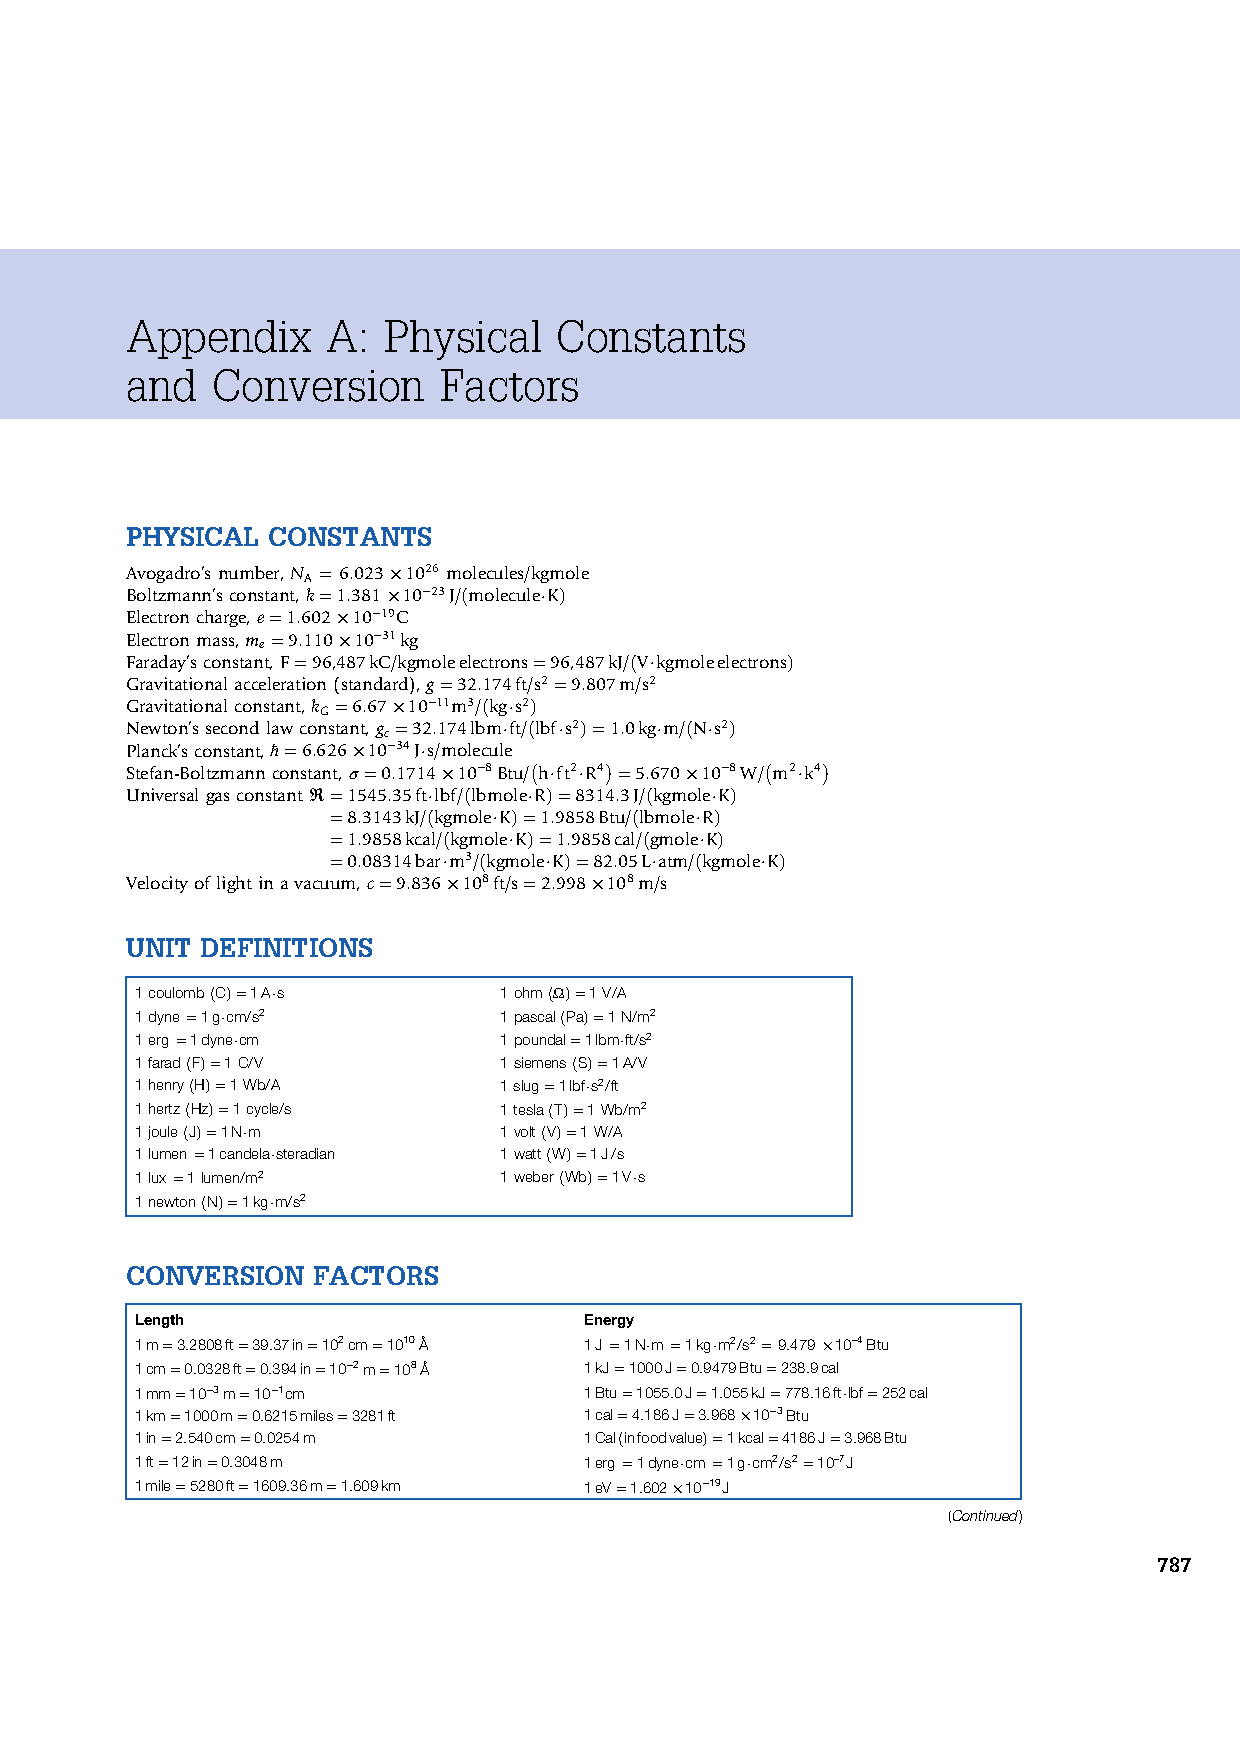
\includepdf[scale=1,pages=-,pagecommand={}, fitpaper]{./../Pics/ChemEng_UnitConv.pdf}

     
\chapter{Table of Properties of Saturated and Superheated Fluids}

Extracted from~\cite{Moran_Book}:\\
  \begin{tabular}{c l}
     \hspace{1cm} & M.J. Moran and H.N. Saphiro \\
                  & Fundamentals of Engineering Thermodynamics \\
                  & John Wiley $\&$ Sons, 5$^{\text{th}}$ Edition  \\
  \end{tabular}

  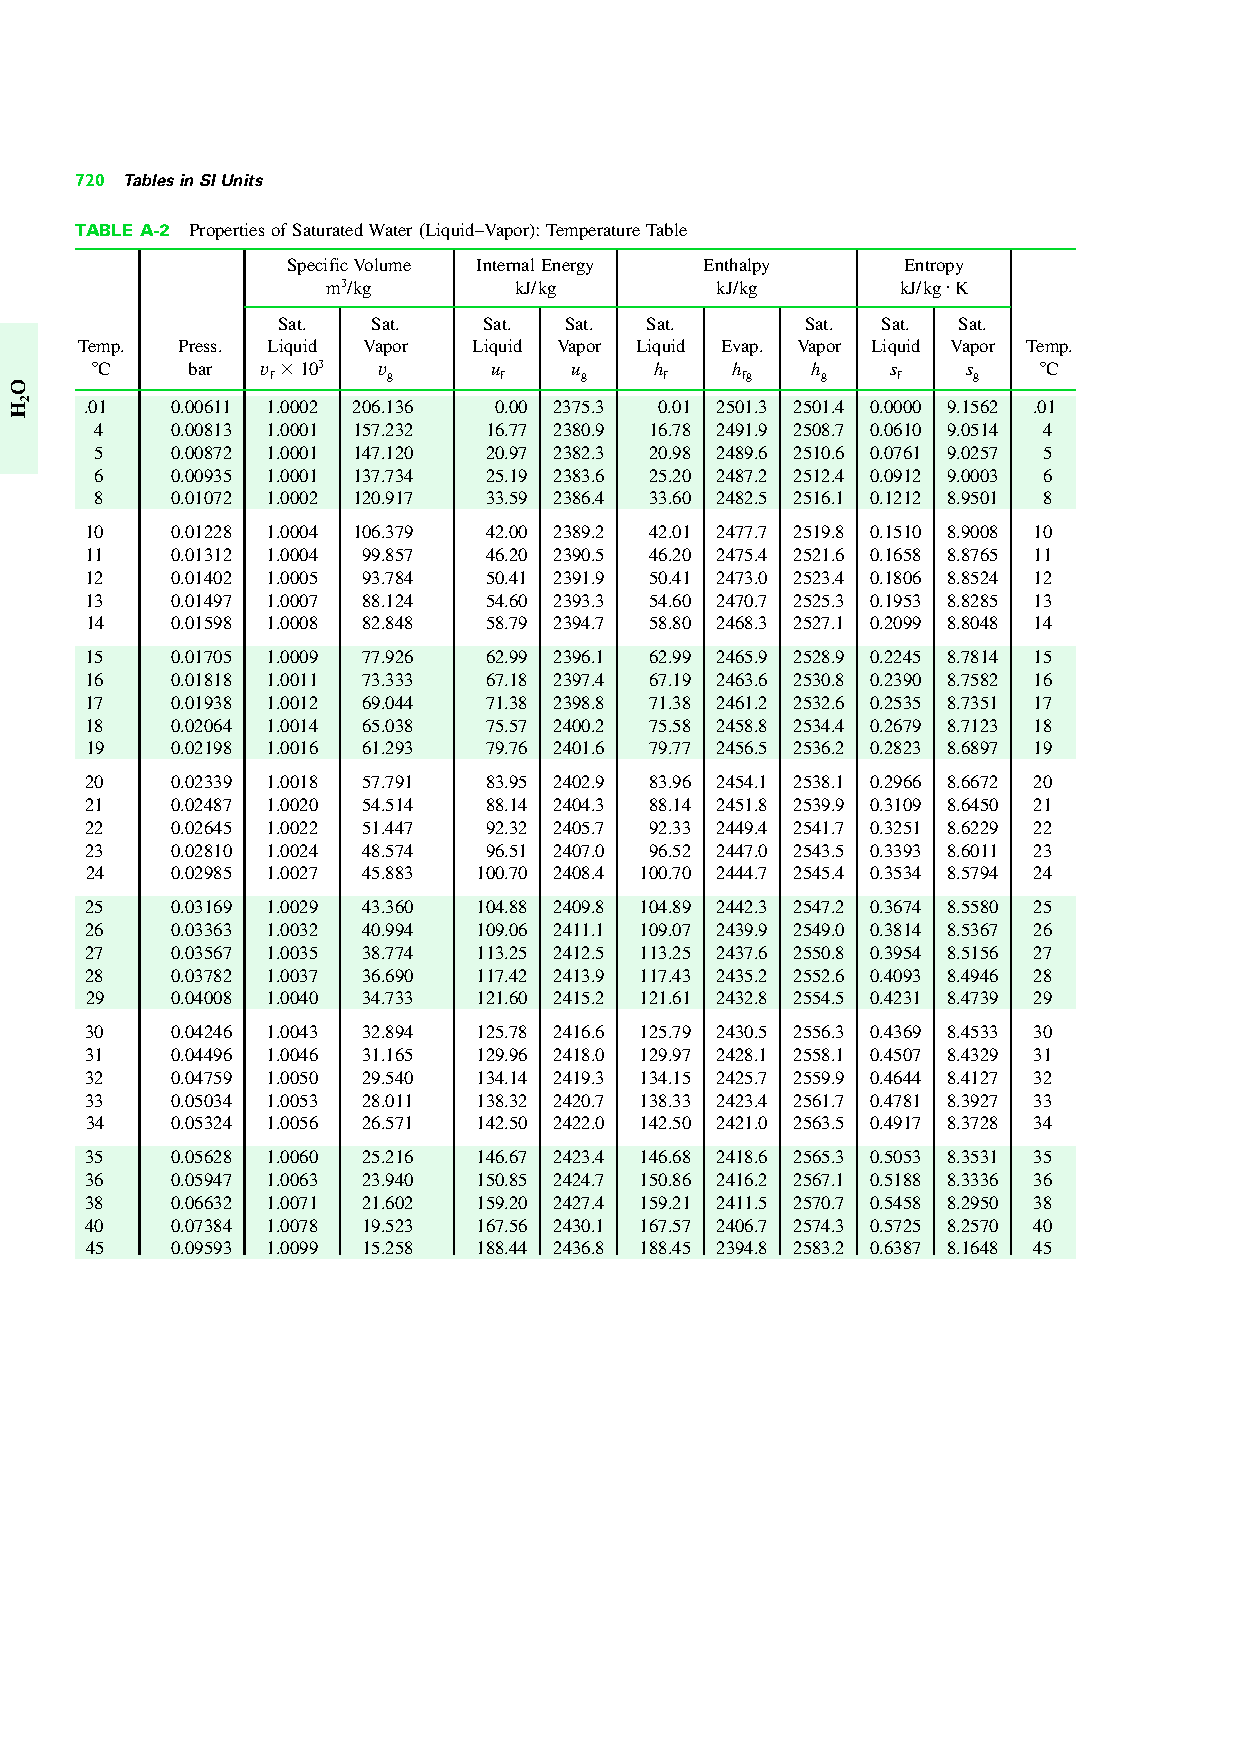
\includepdf[scale=1,pages=-,pagecommand={}, fitpaper]{./Pics/ChemEng_AllTables.pdf}

     
\chapter{Summary of Logarithms and Exponential Properties}
{\it This is not examinable} -- it is here so that you can see where some of the notations, operations and results of earlier sections come from. 

%%%
%%% EXPONENTS
%%%
\section{Exponents}
Assuming that $a$, $b$, $m$ and $n$ are real numbers, the following properties of exponents hold:
\begin{center}
  \begin{tabular}{||c l | c l ||}
    \hline\hline
     1 & $a^{m}a^{n} = a^{m+n}$ & 6 & $\frc{a^{m}}{a^{n}} = a^{m-n}$, $\forall a\neq 0$ \\
     2 & $\left(a^{m}\right)^{n} = a^{mn}$ & 7 &  $\left(ab\right)^{m} = a^{m}b^{m}$ \\
     3 & $\left(\frc{a}{b}\right)^{m} = \frc{a^{m}}{b^{m}}$, $\forall b\neq 0$ & 8 & $a^{-m}=\frc{1}{a^{m}}$, $\forall a\neq 0$ \\
     4 & $a^{1/n} = \sqrt[n]{a}$ & 9 & $a^{0} = 1$, $\forall a\neq 0$ \\
     5 & $a^{m/n} = \sqrt[n]{a^{m}} = \left(\sqrt[n]{a}\right)^{m}$ & & \\ 
    \hline\hline
  \end{tabular}
\end{center}


%%%
%%% LOGARITHMS
%%%
\section{Logarithms}
Let's define $y = \log_{a}x$ if ({\it and only if}) $x=a^{y}$, $\forall a>0$. Given the {\it Euler number}, $e$,
\begin{displaymath}
e = \sum\limits_{n=0}^{\infty}\frc{1}{n!}\sim 2.71828
\end{displaymath}
we can define $\ln x = \log_{e}{x}$, referred as the natural logarithm. The following properties of logarithms hold:
\begin{center}
  \begin{tabular}{||c l | c l||}
     \hline\hline
       1  & $\log_{a}b = \frc{\log_{10}{a}}{\log_{10}{b}}$ & 1' & $\log_{a}b = \frc{\ln{a}}{\ln{b}}$\\
     \hline
       2  & $\log_{a}{xy} = \log_{a}{x}+\log_{a}{y}$ & 2' &$\ln{xy} = \ln{x}+\ln{y}$  \\
     \hline
       3  & $\log_{a}{\frc{x}{y}} = \log_{a}{x}-\log_{a}{y}$ & 3' & $\ln{\frc{x}{y}} = \ln{x}-\ln{y}$ \\
     \hline
       4  & $\log_{a}{x^{y}} = y\cdot\log_{a}{x}$ & 4' & $\ln{x^{y}} = y\cdot\ln{x}$ \\
     \hline
       5  & $\log_{a}{a^{x}} = x$ & 5' & $\ln{e^{x}} = x$ \\
     \hline
       6  & $a^{\log_{a}{x}} = x$   & 6' & $e^{\ln{x}} = x$ \\
     \hline
       7  & $\log_{a}{a} = 1$, $\forall a>0$ & 7' & $\ln{e} = 1$ \\ 
     \hline
       8  & $\log_{a}1 = 0$, $\forall a > 0$ & 8' & $\ln{1} = 0$ \\
     \hline\hline
  \end{tabular}  
\end{center}

     
\chapter{Calculus' Background for Thermodynamics}\label{Appendix_Calculus}
{\it This is not examinable} -- it is here so that you can see where some of the notations, operations and results of earlier sections came from. Details of the contents of this Appendix can be found in \cite{Leithold_Book,Kallo_1955,Strang_Book} or in any {\it Calculus} text-book.
\bigskip

%%%
%%% SECTION
%%%
\section{Vector Calculus}

The operator {\it del} (or {\it nabla}),\index{{\it del} ($\nabla$) operator}\index{{\it nabla} ($\nabla$) operator}\index{$\nabla$}
\begin{displaymath}
  \nabla \equiv \left(\frc{\partial}{\partial x}, \frac{\partial}{\partial y}, \frac{\partial}{\partial z}\right)
\end{displaymath} 
is both a vector and a differential operator and can be used to define,
\begin{enumerate}
%
  \item Gradient: operates on a scalar field $\phi$, e.g., $T$, $\rho$, $\cdots$\index{Gradient}
     \begin{displaymath}
        \text{grad}\phi \equiv \nabla\phi \equiv \left(\frc{\partial\phi}{\partial x}, \frac{\partial\phi}{\partial y}, \frac{\partial\phi}{\partial z}\right)
     \end{displaymath}
%
  \item Divergence: operates on a vector field  $\theta = \left(\theta_{x}, \theta_{y}, \theta_{z}\right) $, e.g., velocity field.\index{Divergence}
     \begin{displaymath}
        \text{div}\theta \equiv \nabla\cdot\theta \equiv \frc{\partial\theta_{x}}{\partial x} + \frac{\partial\theta_{y}}{\partial y} + \frac{\partial\theta_{z}}{\partial z}
     \end{displaymath}
%
  \item Curl: operates on a vector field  $\theta = \left(\theta_{x}, \theta_{y}, \theta_{z}\right)$,\index{Curl}
     \begin{displaymath}
        \text{curl}\theta \equiv \nabla\times\theta \equiv \begin{pmatrix} i & j & k \\ \frc{\partial}{\partial x} & \frc{\partial}{\partial y} & \frc{\partial}{\partial z} \\ \theta_{x} & \theta_{y} & \theta_{z} \end{pmatrix}
     \end{displaymath}
%
   \item Laplacian: operates on a scalar field $\phi$,\index{Laplacian}
      \begin{displaymath}
         \text{div}\left(\text{grad}\phi\right) \equiv \nabla\cdot\nabla\phi \equiv \nabla^{2}\phi \equiv \frc{\partial^{2}\phi}{\partial x^{2}} + \frc{\partial^{2}\phi}{\partial y^{2}} + \frc{\partial^{2}\phi}{\partial z^{2}}
      \end{displaymath}
%
\end{enumerate}


%%%
%%% SECTION
%%%
\section{Some Basic Derivatives/Integration Operations}

\begin{center}
  \begin{tabular}{|| l l | l l ||}
    \hline\hline
       {\bf f(x)}  & {\bf f'(x)}  & {\bf f(x)}  & {\bf f'(x)}  \\
    \hline\hline
       $x^{n}$      &  $nx^{n-1}$   & $\ln{x}$    & $x^{-1}$      \\
       $e^{x}$      &  $e^{x}$      & $sin(x)$   & $cos(x)$     \\
       $cos(x)$    &  $-sin(x)$   & $tan(x)$    & $sec^{2}(x)$  \\
    \hline\hline
       {\bf f(x)}  &  {\bf $\int$f(x)dx} & {\bf f(x)}  &  {\bf $\int$f(x)dx} \\
    \hline\hline
       $e^{x}$      & $e^{x}+\mathcal{C}$& $x^{n}$ for $n\neq -1$ & $\frc{x^{n+1}}{n+1}+\mathcal{C}$ \\
                    &                  &                        & \\
       $1/x$ for $x\neq 0$& $\ln{|x|}+\mathcal{C}$ & $a^{x}$ for $a\neq 1$, $a>0$ & $\frc{a^{x}}{\ln{a}}+\mathcal{C}$\\
                   &                  &                         & \\
       $e^{ax}$ for $a\neq 0$  & $\frc{e^{ax}}{a}+\mathcal{C}$ & $cos(ax)$ for $a\neq0$ & $\frc{1}{a}sin(ax)+\mathcal{C}$\\
                   &                  &                        & \\
       $sin(ax)$ for $a\neq 0$ & $-\frc{1}{a}cos(ax)+\mathcal{C}$& & \\
    \hline\hline
  \end{tabular}
\end{center}

\begin{itemize}
%
  \item Derivative of a sum:
    \begin{displaymath}
       \frc{d}{dx}\left[f(x)+g(x)\right] = \frc{d}{dx}f(x) + \frc{d}{dx}g(x) = f'(x)+g'(x) 
    \end{displaymath}
%
  \item Derivative with a constant factor $c$:
    \begin{displaymath}
       \frc{d}{dx}\left[c f(x)\right] = c\frc{d}{dx}f(x) = cf'(x)
    \end{displaymath}
%
  \item Derivative of a product:
    \begin{displaymath}
       \frc{d}{dx}\left[f(x)g(x)\right] = f(x)g'(x) + f'(x)g(x)
    \end{displaymath}
%
  \item Derivative of a quotient:
    \begin{displaymath}
      \frc{d}{dx}\left[\frc{f(x)}{g(x)}\right] = \frc{g(x)f'(x)-f(x)g'(x)}{g^{2}(x)}
    \end{displaymath}
%
  \item Chain rule (or function of a function):
    \begin{displaymath}
      \frc{d}{dx}f\left[g(x)\right] = f'\left[g(x)\right]g'(x)
    \end{displaymath}
%
  \item Chain rule of a linear function:
    \begin{displaymath}
      \frc{d}{dx} \left[f(ax+b)\right] = a f'(ax+b)
    \end{displaymath}
%
  \item Integral of a function of a linear function:
    \begin{displaymath}
       \int\left[f'(ax+b)\right]dx = \frc{1}{a}f(ax+b) + \mathcal{C}
    \end{displaymath}
%
  \item Integral of a chain rule derivative:
    \begin{displaymath}
       \int\left\{f'\left[g(x)\right]g'(x)\right\}dx = f\left[g(x)\right] + \mathcal{C}
    \end{displaymath}
%
  \item Integral of a sum:
    \begin{displaymath}
      \int\left[f(x)+g(x)\right]dx = \int f(x)dx + \int g(x)dx
    \end{displaymath}
%
  \item Integral with a constant function:
    \begin{displaymath}
       \int c f(x)dx = c\int f(x)dx
    \end{displaymath}
%
  \item Integration by parts:
    \begin{displaymath}
       \int\left[f(x)g'(x)\right]dx = f(x)g(x) - \int\left[f'(x)g(x)\right]dx
    \end{displaymath}
%
  \item Definite integral (if $f'(x)$ is continuous at $a<x<b$):
    \begin{eqnarray}
       && \int\limits_{a}^{b}f(x)dx = - \int\limits_{b}^{a}f(x)dx \nonumber \\
       && \int\limits_{a}^{b}f'(x)dx = \left.f(x)\right|_{a}^{b} = \lim_{x\rightarrow b^{-}}f(x)-\lim_{x\rightarrow a^{+}}f(x)\nonumber
    \end{eqnarray}
%
  \item Substitution:
    \begin{eqnarray}
        \int f(x)dx = \int f(x(u))\frc{dx}{du}du && \text{(indefinite integral)} \nonumber \\
        \int\limits_{a}^{b} f(x) = \int\limits_{u(a)}^{u(b)}f(x(u))\frc{dx}{du}du  && \text{(definite integral)} \nonumber
    \end{eqnarray}
%
  \item Integration by parts:
    \begin{eqnarray}
       \int f(x)g'(x)dx = f(x)g(x) - \int f'(x)g(x) && \text{(indefinite integral)} \nonumber \\
       \int\limits_{a}^{b} f(x)g'(x)dx = \left.f(x)g(x)\right|_{a}^{b} - \int\limits_{a}^{b} f'(x)g(x) && \text{(definite integral)} \nonumber        
    \end{eqnarray}
%
\end{itemize}


%%%
%%% SECTION
%%%
\section{Partial Derivatives and Total Differentials}

%%% SUBSECTION
\subsection{Partial Derivatives:} Given a function $\phi\left(x_{1},x_{2},x_{3},\cdots,x_{n-1},x_{n}\right)$ of $n$ independent variables, the partial derivative of $\phi$ with respect to $x_{i}$, holding the other $n-1$ independent variables constant, is defined as,
  \begin{displaymath}
    \left(\frc{\partial\phi}{\partial x_{i}}\right)_{x_{j\neq i}} = \lim_{\Delta x_{i}\rightarrow 0}\left\{\frc{\phi\left(x_{1},x_{2},\cdots,x_{i}+\Delta x_{i},\cdots,x_{n}\right)-\phi\left(x_{1},x_{2},\cdots,x_{i},\cdots,x_{n}\right)}{\Delta x_{i}}\right\}
  \end{displaymath}

{\bf Example:} A pure fluid with ideal gas behaviour, the pressure can be expressed as a function of the number of mols ($n$), volume ($V$) and temperature ($T$),
  \begin{displaymath}
     P(n,V,T) = \frc{n R T}{V},
  \end{displaymath}
thus,
  \begin{displaymath}
     \left(\frc{\partial P}{\partial n}\right)_{V,T} = \frc{RT}{V}\hspace{1cm} \left(\frc{\partial P}{\partial V}\right)_{n,T} = -\frc{n R T}{V^{2}} \hspace{1cm} \left(\frc{\partial P}{\partial T}\right)_{n,V} = \frc{n R}{V}\d{T}
  \end{displaymath}


%%% SUBSECTION
\subsection{Total Differentials:} Given a function $\phi\left(x_{1},x_{2},x_{3},\cdots,x_{n-1},x_{n}\right)$ of $n$ independent variables, the {\it total differential} of $\phi$, $d\phi$, is defined as
  \begin{eqnarray}
     d\phi &=& \sum\limits_{i=1}^{n}\left(\frc{\partial \phi}{\partial x_{i}}\right)_{x_{j\neq i}} d x_{i} \nonumber \\
     &=& \left(\frc{\partial\phi}{\partial x_{1}}\right)_{x_{2},\cdots,x_{n}} d x_{1} + \left(\frc{\partial\phi}{\partial x_{2}}\right)_{x_{1},x_{3},\cdots,x_{n}} dx_{2} + \cdots +  \left(\frc{\partial\phi}{\partial x_{n}}\right)_{x_{1},x_{2},\cdots,x_{n-1}} d x_{n} \nonumber 
  \end{eqnarray}
where $d x_{i}$ is an infinitesimal small increment in $x_{i}$.

\noindent
{\bf Example:} Infinitesimal changes in the ideal gas pressure are expressed as,
  \begin{eqnarray}
      d P &=& \left(\frc{\partial P}{\partial n}\right)_{V,T}\d{n} + \left(\frc{\partial P}{\partial V}\right)_{n,T}\d{V} + \left(\frc{\partial P}{\partial T}\right)_{n,V}\d{T} \nonumber \\
     &=& \frc{R T}{V} d n - \frc{n R T}{V^{2}} d V + \frc{n R}{V} d T. \nonumber 
  \end{eqnarray}

%%% SUBSECTION
\subsection{Properties of Partial Derivatives}\label{Appendix_Calculus:Properties}
  \begin{enumerate}[(i)]
%
     \item The order of differentiation in mixed second derivatives is immaterial, i.e.,
        \begin{displaymath}
           \left[\frc{\partial}{\partial y}\left(\frc{\partial\phi}{\partial x}\right)_{y}\right]_{x} = \left[\frc{\partial}{\partial x}\left(\frc{\partial\phi}{\partial y}\right)_{x}\right]_{y} \hspace{1cm}\Longleftrightarrow\hspace{1cm} \frc{\partial^{2}\phi}{\partial x\partial y} = \frc{\partial^{2}\phi}{\partial y\partial x}
        \end{displaymath}
%
     \item Cyclic rule:
        \begin{displaymath}
           \left(\frc{\partial\phi}{\partial x}\right)_{y}\left(\frc{\partial y}{\partial \phi}\right)_{x}\left(\frc{\partial x}{\partial y}\right)_{\phi} = -1
        \end{displaymath}
%
     \item Given $\phi(x,y)$ and $\varphi(x,y)$:
        \begin{enumerate}[(a)]
           \item $\left(\frc{\partial\phi}{\partial\varphi}\right)_{x} = \left(\frc{\partial\phi}{\partial y}\right)_{x}\left(\frc{\partial y}{\partial\varphi}\right)_{x}$  (chain rule);
           \item $\left(\frc{\partial\phi}{\partial x}\right)_{\varphi} = \left(\frc{\partial\phi}{\partial x}\right)_{y} + \left(\frc{\partial\phi}{\partial y}\right)_{x}\left(\frc{\partial y}{\partial x}\right)_{\varphi} $
        \end{enumerate}  
%
  \end{enumerate}

%%%
%%% SECTION
%%%
\section{The Mean Value Theorem and l'H\^opital's Rule}\label{Appendix:lHopital}

\begin{theorem}[Mean value]\index{Mean value theorem}\label{Appendix:MeanValueTheorem}
Suppose $f(x)$ is continuous in the closed interval $a\leq x\leq b$ and has derivatives everywhere in the open interval $a<x<b$. Then,
     \begin{equation}
       \frc{f(a)-f(b)}{b-a} = f'(c)\;\;\;\text{ at some point } a<c<b.
     \end{equation}
\end{theorem}

\begin{theorem}[Rolle's theorem, i.e., extrema of a function]\index{Mean value theorem ! Rolle's theorem}
   Suppose $f(a) = f(b) = 0$ (zero at endpoints). Then $f'(c) = 0$ at some point within $a<c<b$.
\end{theorem}

\begin{theorem}[l'H\^opital rule]\index{Mean value theorem ! L'H\^opital rule}\index{L'H\^opital rule}
   Suppose $f(x)$ and $g(x)$ are differentiable and $g'(x)\neq 0$ near a point $a$ (except possibly at $a$). Suppose that
    \begin{displaymath}
      \lim_{x\rightarrow a} f(x) = 0 \;\;\text{ and }\;\; \lim_{x\rightarrow a} g(x) = 0,
    \end{displaymath}
or that
    \begin{displaymath}
      \lim_{x\rightarrow a} f(x) = \pm\infty \;\;\text{ and }\;\; \lim_{x\rightarrow a} g(x) = \pm\infty,
    \end{displaymath}
$\left(\text{i.e., an indeterminate quotient, }\frc{0}{0} \text{ or }\frc{\infty}{\infty}\right)$. Then
    \begin{equation}
        \lim_{x\rightarrow a}\frc{f(x)}{g(x)} = \lim_{x\rightarrow a}\frc{f'(x)}{g'(x)},
    \end{equation}
if the limit on the right side exists (or is $\infty$ or $-\infty$).
%both approach zero as $x\rightarrow a$. Then $\frc{f(x)}{g(x)}$ approaches the same limit as $\frc{f'(x)}{g'(x)}$, if this second limit exists,
%    \begin{equation}
%        \lim_{x\rightarrow a}\frc{f(x)}{g(x)} = \lim_{x\rightarrow a}\frc{f'(x)}{g'(x)}.
%    \end{equation}
%   This limit often is $\frc{f'(a)}{g'(a)}$.
    \begin{list}{\bf Example \arabic{qcounter}:~}{\usecounter{qcounter}}
%       
       \item Find $\lim\limits_{x\rightarrow\infty} \frc{5x-2}{7x+3}$.
           \begin{eqnarray}
              \lim_{x\rightarrow\infty}\frc{5x-2}{7x+3} &=& \frc{\infty}{\infty} \nonumber \\
                                                   &=& \lim_{x\rightarrow\infty}\frc{\left[5x-2\right]'}{\left[7x+3\right]'} = \lim_{x\rightarrow\infty} \frc{5}{7} = \frc{5}{7}\nonumber
           \end{eqnarray}
%
      \item Find $\lim\limits_{x\rightarrow -2}\frc{x+2}{\ln{(x+3)}}$. 
           \begin{eqnarray}
              \lim_{x\rightarrow -2}\frc{x+2}{\ln{(x+3)}} &=& \frc{0}{0} \nonumber \\                                                   &=& \lim_{x\rightarrow -2}\frc{\left[x+2\right]'}{\left[\ln{(x+3)}\right]} = \lim_{x\rightarrow -2} \frc{1}{\frc{1}{x+3}} = \lim_{x\rightarrow -2} \left(x+3\right) = 1 \nonumber
           \end{eqnarray}
         
%
    \end{list}


\end{theorem}

%%%
%%% SECTION
%%%
\section{Line Integrals}\index{Line integral}

%%%
\subsection{Exact and Inexact Differential}\index{Line integral!Exact differential}\index{Line integral!Inexact differential}
Consider that $\mathbf{\Psi}$ is a function of the independent variables $x_{j}$ (with $j=1,2,\cdots,n$),  $\Psi_{i}=\Psi_{i}\left(x_{1},x_{2},\cdots,x_{n}\right)$. An infinitesimal quantity,
   \begin{displaymath}
      dz = \sum\limits_{i=1}^{n} \Psi_{i}\left(x_{1},x_{2},\cdots,x_{n}\right) d x_{i} =  \Psi_{1} d x_{1} + \Psi_{2} d x_{2} +\cdots + \Psi_{n} d x_{n},
   \end{displaymath}
is called {\it linear differential}\index{Linear differential}. If we focus on a two-dimensional problem, i.e., $\mathbf{\Psi}=\left\{M(x,y),N(x,y)\right\}$,
   \begin{equation}
      dz = M d x + N d y\label{Appendix_Calculus:Eqn:ExactLinearDifferential}
   \end{equation}

\medskip
Equation~\ref{Appendix_Calculus:Eqn:ExactLinearDifferential} is an {\it exact differential}\index{Exact differential} if, and only if, there is a function of $x$ and $y$, $\Phi(x,y)$, such that $d \Phi= d z$ for all values of $x$ and $y$. This is equivalent to
   \begin{displaymath}
        \Partial[M]{y}{x} = \Partial[N]{x}{y}.
   \end{displaymath}
The equation
   \begin{equation}
      dw = M^{\prime} d x + N^{\prime} d y,\label{Appendix_Calculus:Eqn:InexactLinearDifferential}
   \end{equation}
 is an {\it inexact differential}\index{Inexact differential} if, and only if, there is no function $\Phi(x,y)$, such that $d \Phi = d w$ for all values of $x$ and $y$, thus,
   \begin{displaymath}
        \Partial[M^{\prime}]{y}{x} \neq \Partial[N^{\prime}]{x}{y}.
   \end{displaymath}

%%%
\subsection{Fundamental Theorem for Line Integrals}\index{Line integral!Fundamental theorem}

\begin{theorem}
   If {\bf F} is a gradient or conservative vector field, i.e., $\mathbf{F}=\mathbf{\nabla}f(x,y)=\langle f_{x}, f_{y}\rangle$ for a {\it potential function} $f$ for the field, and $\mathcal{C}$ is a curve with endpoints $P_{0}=\left(x_{0},y_{0}\right)$ and $P_{1}=\left(x_{1},y_{1}\right)$,
      \begin{eqnarray}
         \int\limits_{\mathcal{C}}\mathbf{F}\cdot d\mathbf{r} &=& \int\limits_{\mathcal{C}}\mathbf{\nabla}f d \mathbf{r} = \left.f(x,y)\right|_{P_{0}}^{P_{1}}\\
                                                           &=& f\left(P_{1}\right)-f\left(P_{0}\right) = f\left(x_{1},y_{1}\right) - f\left(x_{0},y_{0}\right)\nonumber.
      \end{eqnarray}
\end{theorem} 
That is, for gradient fields the line integral is independent of the path taken, i.e., it depends only on the endpoints of $\mathcal{C}$. We call such a line integral {\it path independent}.
\medskip

The line integral of a vector field over a {\it simple} (i.e., non-intersecting) {\it closed} (i.e., no endpoints) curve $\mathcal{C}$ is denoted as,\index{Line integral}
        \begin{equation}
           \oint_{\mathcal{C}}\mathbf{F}\cdot d \mathbf{r} = 0,
        \end{equation}
i.e., the line integral around all closed paths is 0 $\leftrightarrow$ -- {\it path independence}.

     
\chapter{Introduction to Numerical Methods relevant to Thermodynamics}\label{Appendix_NumMethods}

{\it This is not examinable} -- it is here so that you can see where some of the notations, operations and results of earlier sections came from. Details of the contents of this Appendix can be found in \cite{Atkinson_Book_Newton,Atkinson_Book_Interpolation,NumericalRecipes_Interpolation,NumericalRecipes_Newton} or in any text-book of {\it Mathematical or Numerical Methods} for engineering.

%%%
%%% SECTION
%%%
\section{Linear Interpolation}\label{LinearInterpolation}\index{Linear interpolation}

Given a continuous and unknown function $f(x)$, defined at a set of points  $x_{1} < \cdots < x_{i} < \cdots < x_{N}$. Interpolation is the process of determining a polynomial expression to calculate the pair $\left[x_{k}, f\left(x_{k}\right)\right]$ based on neighbours discrete coordinates $\left\{\left[x_{1},f\left(x_{1}\right)\right], \cdots, \left[x_{N},f\left(x_{N}\right)\right]\right\}$. 

Consider a set of discrete data points,
  \begin{center}
    \begin{tabular}{c | c }
        $\mathbf{x}$   & $\mathbf{f\left(x_{i}\right)}$ \\
        \hline
           $x_{1}$ &  $f\left(x_{1}\right)$ \\
           $x_{2}$ &  $f\left(x_{2}\right)$ \\
           $x_{3}$ &  $f\left(x_{3}\right)$ \\
           $x_{4}$ &  $f\left(x_{4}\right)$ \\
    \end{tabular}
  \end{center}
that are a subset of a continuous and smooth function $y=f(x)$ (Fig.~\ref{Appendix:Fig:Interpolation}). Polynomials of order $n\ge 1$ can be generated to represent this function. High-order polynomials can more accurately fit the discrete coordinatess than low-order polynomials. In Fig.~\ref{Appendix:Fig:Interpolation}, let's assume the discrete pairs 
  \begin{displaymath}
     \left\{\left[x_{1},f\left(x_{1}\right)\right], \left[x_{2},f\left(x_{2}\right)\right],\left[x_{3},f\left(x_{3}\right)\right], \left[x_{4},f\left(x_{4}\right)\right]\right\}
  \end{displaymath}
are known, and one wants to determine the value of the function $f$ at $x_{2} < x_{k} < x_{3}$. If the interval $\Delta x= x_{3}-x_{2}$ is sufficiently small, a linear function can be used to fit these coordinates,
   \begin{displaymath}
       f\left(x_{k}\right) = f\left(x_{2}\right) + m\left(x_{k}-x_{2}\right),%\label{LinearInterpolation:Eqn1}
   \end{displaymath}
where 
   \begin{displaymath}
      m = \frc{f\left(x_{3}\right)-f\left(x_{2}\right)}{x_{3}-x_{2}}.
   \end{displaymath}
If $m$ is replaced in the previous equation, %Eqn.~\ref{LinearInterpolation:Eqn1},
   \begin{displaymath}
       f\left(x_{k}\right) = \frc{f\left(x_{2}\right)\left(x_{3}-x_{k}\right) + f\left(x_{3}\right)\left(x_{k}-x_{2}\right)}{x_{3}-x_{2}}.
   \end{displaymath}
   
   \begin{shaded}
      Or for a general case with $x_{a} < x_{k} < x_{b}$,
        \begin{equation}\label{LinearInterpolation:Eqn1}
            f\left(x_{k}\right) = \frc{f\left(x_{a}\right)\left(x_{b}-x_{k}\right) + f\left(x_{b}\right)\left(x_{k}-x_{a}\right)}{x_{b}-x_{a}}.
        \end{equation}
   \end{shaded}

%%% Figure
     \begin{figure}[h]\label{Appendix:Fig:Interpolation}%
        \begin{center}
          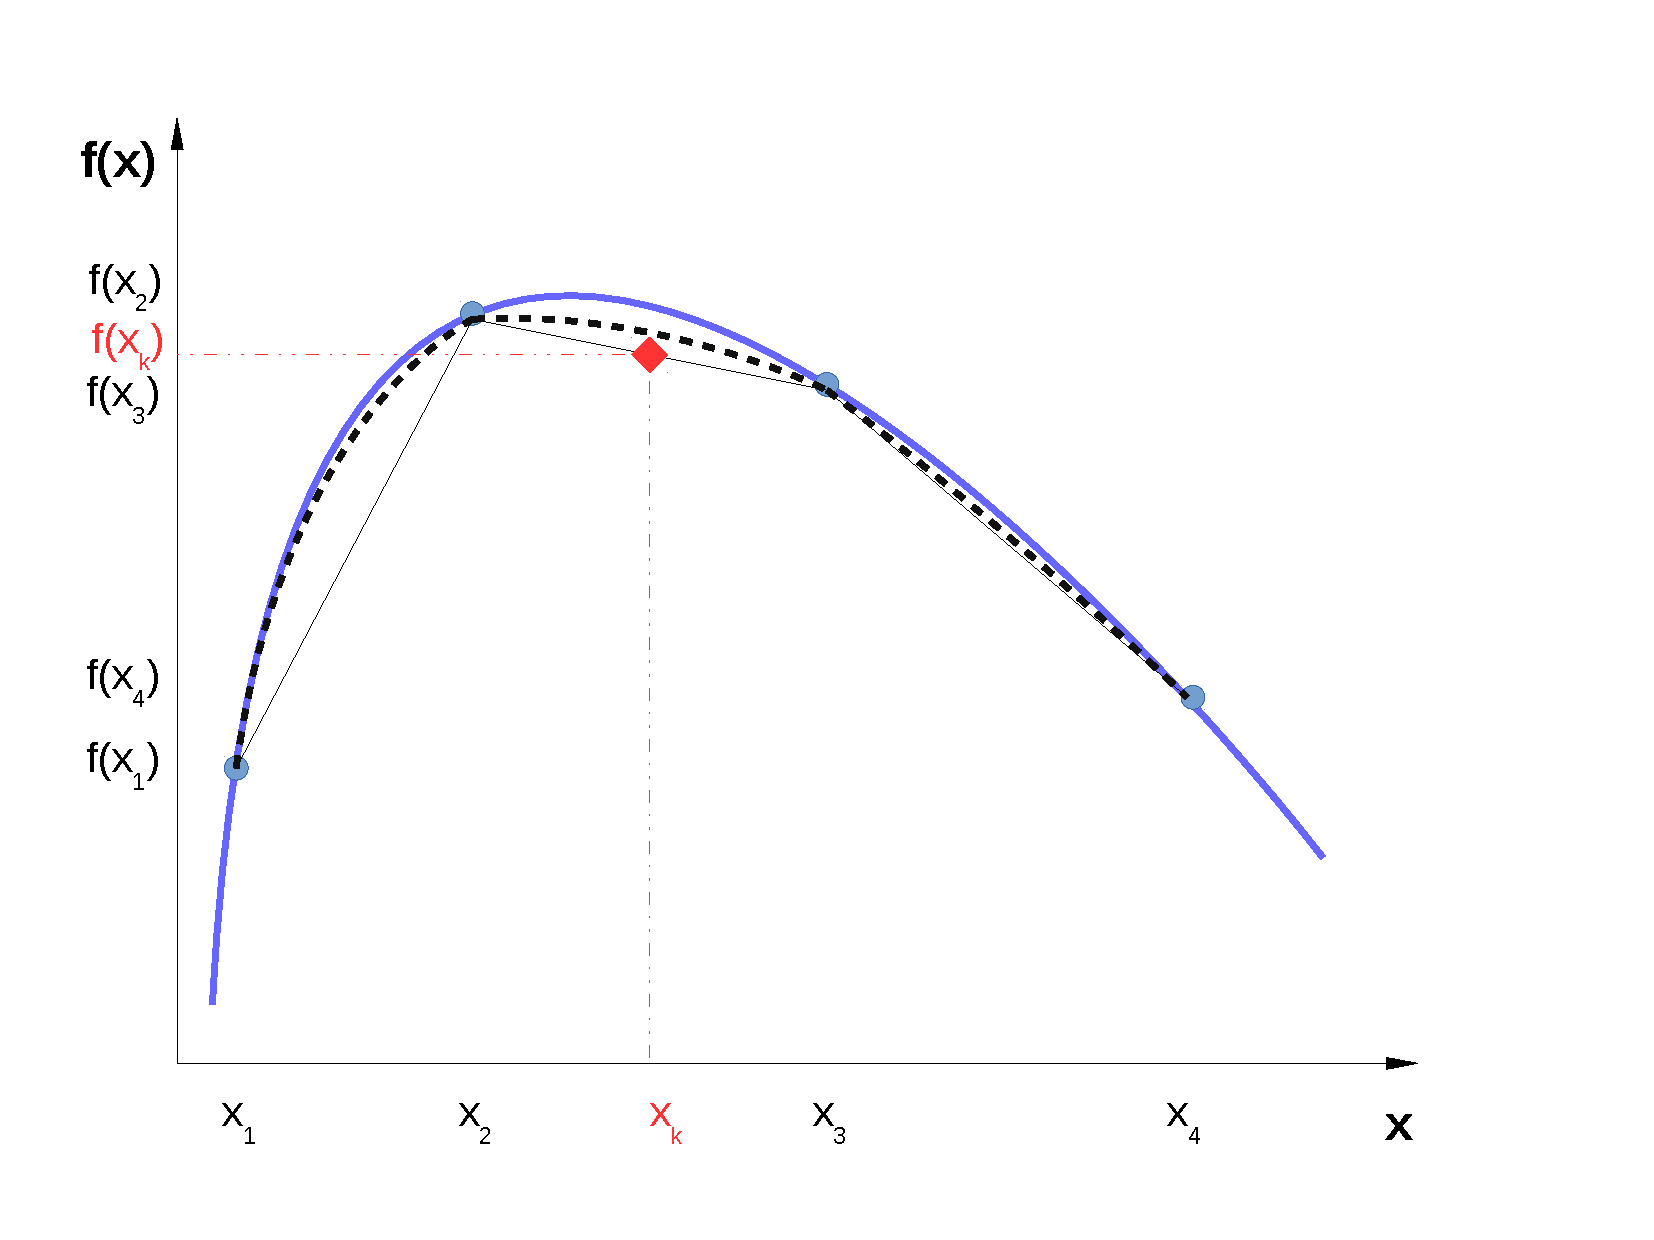
\includegraphics[width=\columnwidth,clip]{./../Pics/Interpolation}
           \caption{Smooth function $f(x)$ (solid blue line) may be more accurately interpolated by a high-order polynomial (black dotted line) than by a low-order polynomial (solid black line).} 
        \end{center}
      \end{figure}

    \begin{list}{\bf Example \arabic{qcounter}:~}{\usecounter{qcounter}}
%       
         \item Given a table of values for $f(x)=\tan{x}$ for a few values of $x$,
            \begin{center}
               \begin{tabular}{c | c c c c}
                   $x$        & 1.00   & 1.10   & 1.20   & 1.30   \\
                   \hline
                   $\tan{x}$  & 1.5574 & 1.9648 & 2.5722 & 3.6021 \\
               \end{tabular}
            \end{center}
            Estimate $\tan{1.15}$ and $\tan{1.23}$.

            {\bf Solution:} For $\left(x_{a}=1.10\right) < \left(x_{k}=1.15\right) < \left(x_{b}=1.20\right)$,
               \begin{eqnarray}
                  f\left(x_{k}\right) &=& \frc{f\left(x_{a}\right)\left(x_{b}-x_{k}\right) + f\left(x_{b}\right)\left(x_{k}-x_{a}\right)}{x_{b}-x_{a}} \nonumber \\
                                     &=& \frc{1.9648\times(1.20-1.15) + 2.5722\times(1.15-1.10)}{1.20-1.10} = 2.2685 \nonumber
               \end{eqnarray}

For  $\left(x_{a}=1.20\right) < \left(x_{k}=1.23\right) < \left(x_{b}=1.30\right)$,
               \begin{eqnarray}
                  f\left(x_{k}\right) &=& \frc{f\left(x_{a}\right)\left(x_{b}-x_{k}\right) + f\left(x_{b}\right)\left(x_{k}-x_{a}\right)}{x_{b}-x_{a}} \nonumber \\
                                     &=& \frc{2.5722\times(1.30-1.23) + 3.6021\times(1.23-1.20)}{1.30-1.20} = 2.8812 \nonumber
               \end{eqnarray}
%
         \item Calculate specific volume $\left(v, \text{in m}^{3}\text{.kg}^{-1}\right)$, internal energy $\left(u, \text{in kJ.kg}^{-1}\right)$ and entropy $\left(s, \text{in kJ.(kg.K)}^{-1}\right)$ of saturated water vapour at 133.45$^{\circ}$C.

           {\bf Solution:} From Appendix~\ref{Appendix:Saturated_SH_Tables} (Table A-2), for $T_{a}(=130.0) < T_{k} (= 133.45) < T_{b} (=140.0)^{\circ}C$, thus:
               \begin{eqnarray}
                  v\left(T_{k}\right) &=& \frc{v\left(T_{a}\right)\left(T_{b}-T_{k}\right) + v\left(T_{b}\right)\left(T_{k}-T_{a}\right)}{T_{b}-T_{a}} \nonumber \\
                                     &=& \frc{0.6685\times(140.0-133.45) + 0.5089\times(133.45-130.0)}{140.0-130.0} = 0.6134 \text{ m}^{3}\text{.kg}^{-1}\nonumber \\
                                     && \nonumber \\
                  u\left(T_{k}\right) &=& \frc{u\left(T_{a}\right)\left(T_{b}-T_{k}\right) + u\left(T_{b}\right)\left(T_{k}-T_{a}\right)}{T_{b}-T_{a}} \nonumber \\
                                     &=& \frc{2539.9\times(140.0-133.45) + 2550.0\times(133.45-130.0)}{140.0-130.0} = 2543.39 \text{ kJ.kg}^{-1}\nonumber \\
                                     && \nonumber \\
                  s\left(T_{k}\right) &=& \frc{s\left(T_{a}\right)\left(T_{b}-T_{k}\right) + s\left(T_{b}\right)\left(T_{k}-T_{a}\right)}{T_{b}-T_{a}} \nonumber \\
                                     &=& \frc{7.0269\times(140.0-133.45) + 6.9299\times(133.45-130.0)}{140.0-130.0} = 6.9934 \text{ kJ.}\left(\text{kg.K}\right)^{-1}\nonumber 
               \end{eqnarray}


    \end{list}

%%%
%%% SECTION
%%%
\section{Root-Finder Methods}\label{Section:RootFinderMethods}\index{Root-Finder Methods}

%%% SUBSECTION
\subsection{Motivation}
Given a smooth, {\it continuous} and {\it fully differentiable} function 
  \begin{displaymath}
     y = f(x) \hspace{3cm} \text{ with } x\in\mathbb{R}.
  \end{displaymath}
We aim to find the root $x=\psi$ of the function 
  \begin{displaymath}
     f(x) = 0.
  \end{displaymath}
The first step is to estimate $x_{0}$ that results in $f\left(x_{0}\right)\neq 0$ and may lead to a new estimate $x_{1}$. The procedure is repeated until $f\left(x_{n}\right)\rightarrow 0$ (\ie $x_{n}\approx\psi$), where $n$ is the number of repetitions (or {\it iterations}). There are several methods designed to solve non-linear equations, i.e., find the rrot of the function, here we will focus on the most popular {\it Newton-Raphson} method that combines simplicity and power.


%%% SUBSECTION
\subsection{Newton-Raphson Iterative Method}\label{Section:RootFinderMethods:NewtonRaphson}\index{Root-Finder Methods!Newton-Raphson method}
Let's assume that $x_{0}$ is a good estimate of the root$\psi$ and $\psi = x_{0} + h$. Since the root of the function $f(x)$ is $\psi$ and $h = \psi 0 x_{0}$, $h$ represents the distance between the initial estimate (or guess) and the root. Assuming $h$ is very (or {\it infinitesimal}) small, we can linearly approximate the function,
   \begin{displaymath}
        f\left(\psi\right) = 0 = f\left(x_{0}+h\right) \approx f\left(x_{0}\right) + h f'\left(x_{0}\right).
   \end{displaymath}
Therefore, except if $f'\left(x_{0}\right)$ is close to $0$, 
   \begin{displaymath}
        h \approx -\frc{f\left(x_{0}\right)}{f'\left(x_{0}\right)} \hspace{.3cm} \Longrightarrow \hspace{.3cm} \psi = x_{0} + h \approx x_{0} -\frc{f\left(x_{0}\right)}{f'\left(x_{0}\right)}.
   \end{displaymath}
%%% Figure
     \begin{figure}[h]\label{Appendix:Fig:NewtonRaphson}%
        \begin{center}
         \vbox{
           \hbox{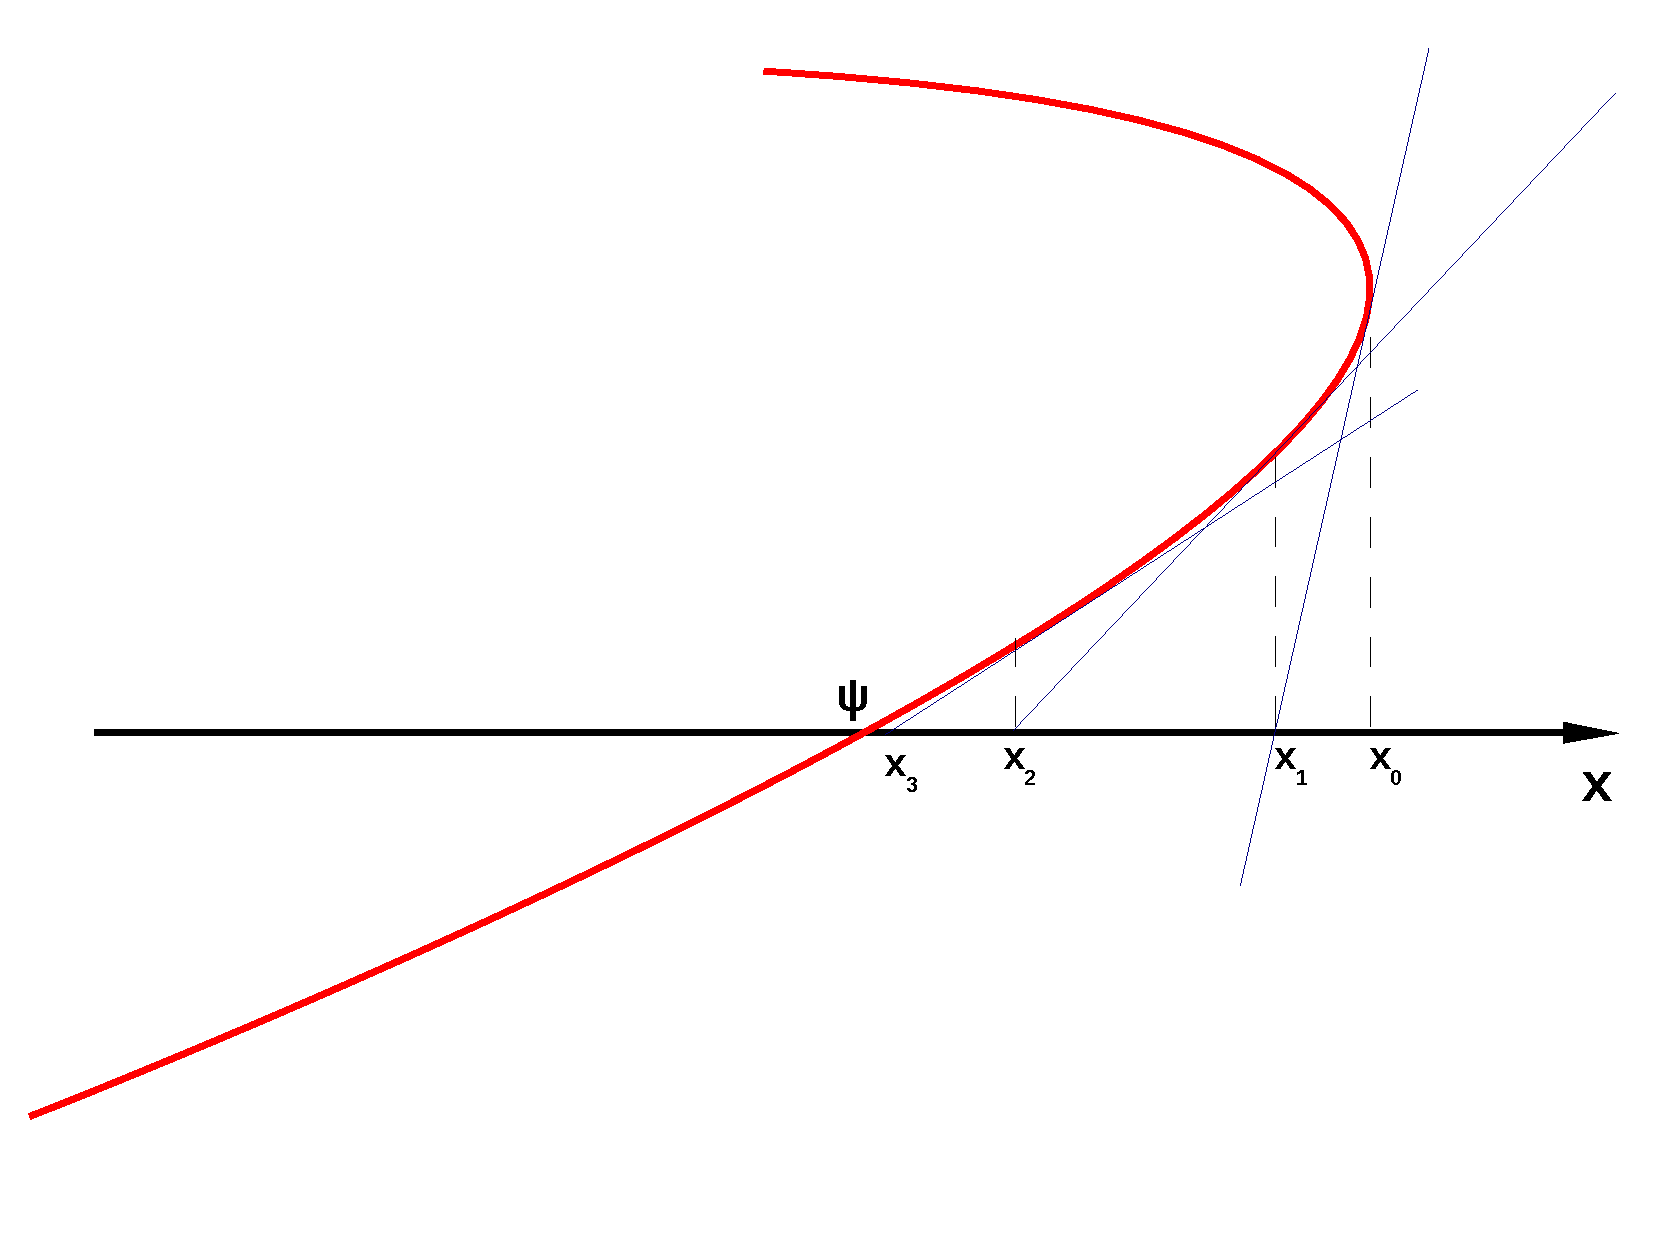
\includegraphics[width=\columnwidth,height=10cm]{./../Pics/NewtonRaphson2}}
           \hbox{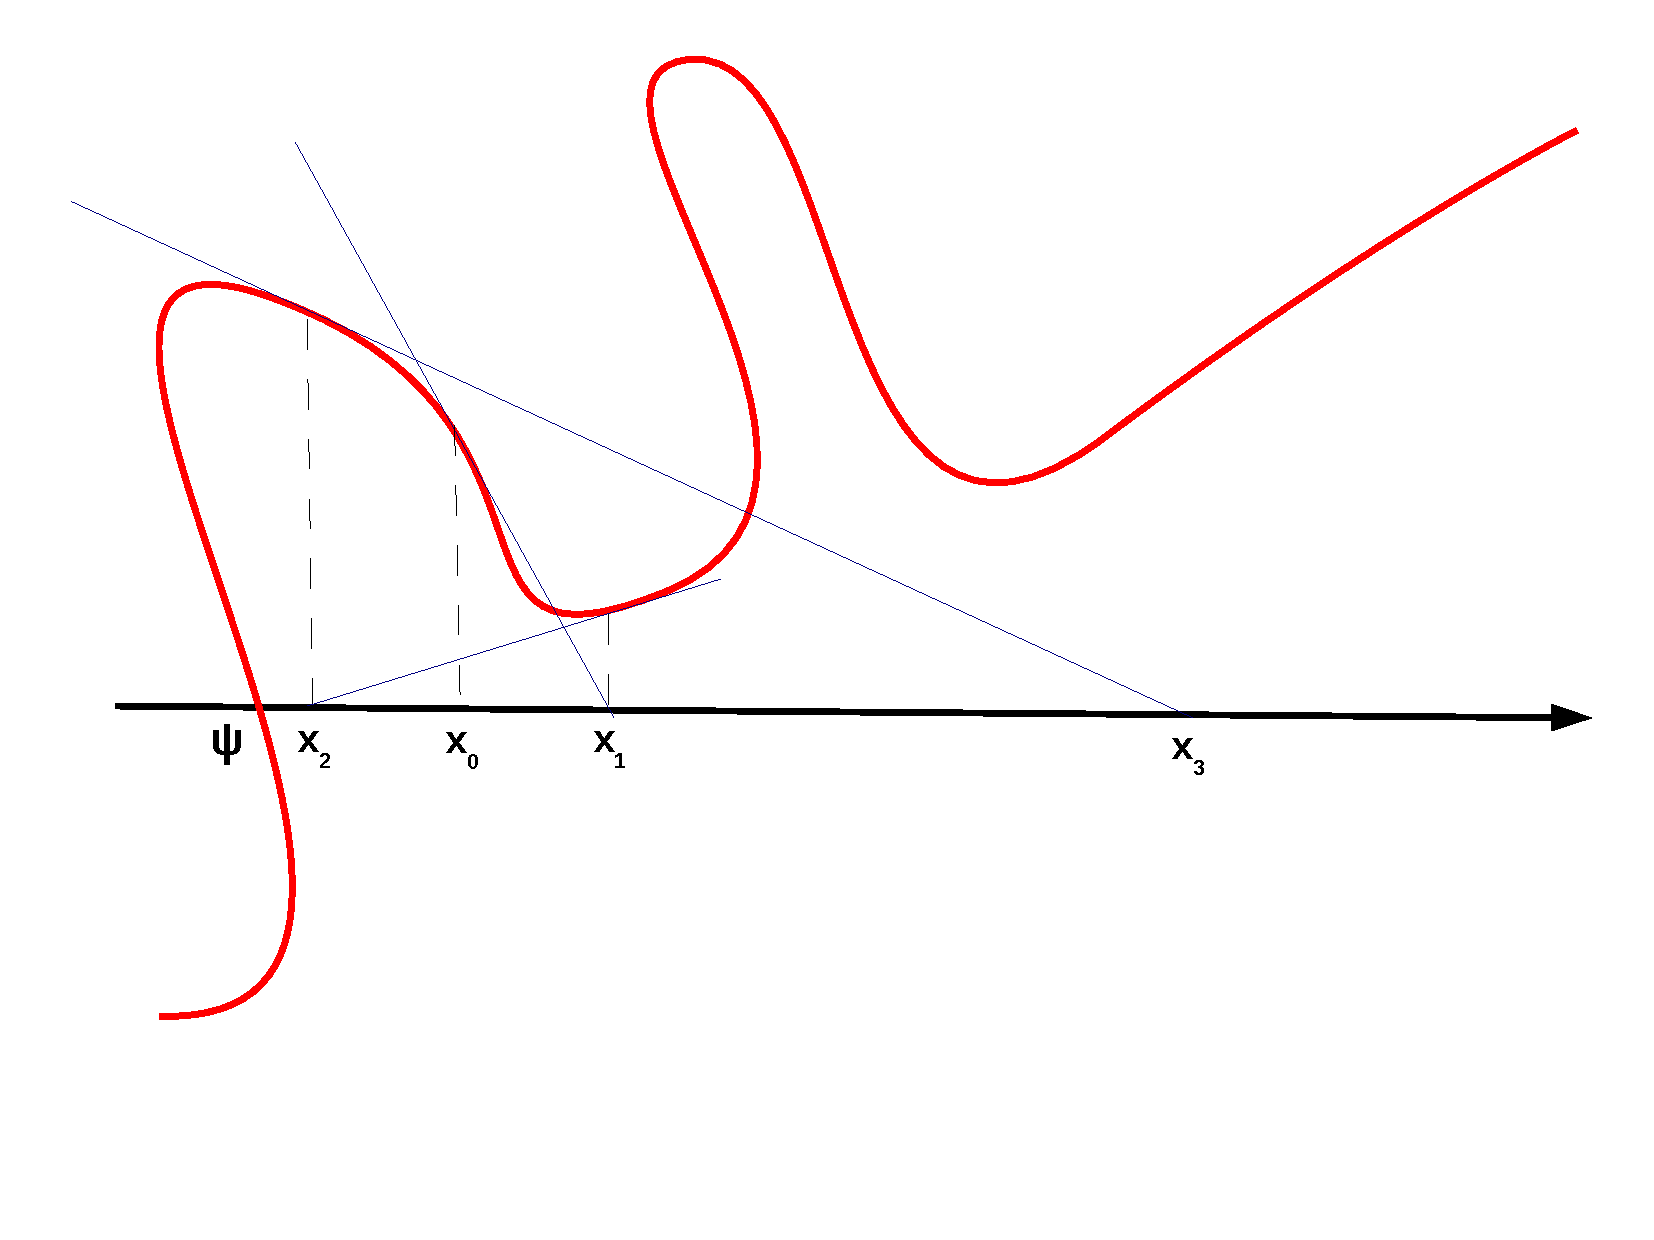
\includegraphics[width=\columnwidth,height=10cm]{./../Pics/NewtonRaphson3}}}
           \vspace{-1cm}
           \caption{Graphic representation of the Newton-Raphson iterative method: (top) solution of the smooth and continuous function $f(x)$ (solid red line) is approximated from the initial estimate $x_{0}$ to the final solution $x=\psi$; (bottom) initial estimate $x_{0}$ is far away from the root $\psi$ and the solution may diverge. Blue solid lines are tangent of the function at $x_{i}$.} 
        \end{center}
      \end{figure}
%
This expression represents an improvement of the original estimate, i.e.,  
   \begin{displaymath}
        x_{1} = x_{0} -\frc{f\left(x_{0}\right)}{f'\left(x_{0}\right)}.
   \end{displaymath}
The next estimate, $x_{2}$, is obtained from $x_{1}$, 
   \begin{displaymath}
        x_{2} = x_{1} -\frc{f\left(x_{1}\right)}{f'\left(x_{1}\right)}.
   \end{displaymath}

   \begin{shaded}
      We can generalise this expression for the $n-${\it th iteration},
         \begin{equation}
            x_{n+1} = x_{n} -\frc{f\left(x_{n}\right)}{f'\left(x_{n}\right)}.\label{NewtonRaphson:Eqn1}
         \end{equation}
   \end{shaded}

Figure~\ref{Appendix:Fig:NewtonRaphson}(a) shows a geometrical representation of the Newton-Raphson iterative method, where $m=f(x)$ is the tangent (blue) line at the coordinate pair $\left[x_{0},f\left(x_{0}\right)\right]$,
   \begin{displaymath}
     m = f\left(x_{0}\right) + \left(x-x_{0}\right)f'\left(x_{0}\right).
   \end{displaymath}
Let $x_{1}$ be the {\it x-intercept} of the tangent line, therefore
   \begin{displaymath}
     x_{1} = x_{0} - \frc{f\left(x_{0}\right)}{f'\left(x_{0}\right)}
   \end{displaymath}
The tangent line is a geometrical representation of the Newton-Raphson iterative method, Eqn.~\ref{NewtonRaphson:Eqn1}, as the estimates gradually tend to the root $\psi$ of the function. As it can be seen in the Fig.~\ref{Appendix:Fig:NewtonRaphson}(b), if the initial estimate $x_{0}$ is not close enough of the root $\psi$, the solution may not {\it converge}. In fact, the Newton-Raphson iterative method works most of the time if the initial estimate is {\it good enough}.

 From the {\it mean value theorem} (Theorem~\ref{Appendix:MeanValueTheorem}), let the function $f(x)$ be such that, 
   \begin{enumerate}[(a)]
      \item it is continuously differentiable in some open interval containing the solution $x=\psi$;
      \item $\left|f'(\psi)\right| < 1$.
   \end{enumerate}
Then there is a number $\epsilon > 0$ such that the iteration $x_{k+1}=f\left(x_{k}\right)$ {\it converges} whenever $x_{0}$ is chosen in $\left|x_{0}-\psi\right|\leq\epsilon$.

For bounded $x\in\mathbb{R}$ (\ie contained in the interval $a\leq x \leq b$), if $f''(x)$ exists and is continuous on $[a,b]$ and $\psi$ is a root of $f(x)$, that is, $f(\psi)=0$ and $f'(\psi)\neq0$. Thus for a function $g(x)$
    \begin{displaymath}
        g(x) = x - \frc{f(x)}{f'(x)}
    \end{displaymath}
with
    \begin{displaymath}
        g'(x) = 1 - \frc{[f'(x)]^{2} - f(x)f''(x)}{[f'(x)]^{2}} = \frc{f(x)f''(x)}{[f'(x)]^{2}},
    \end{displaymath}
and
    \begin{displaymath}
        g'(\psi) = \frc{f(\psi)f''(\psi)}{[f'(\psi)]^{2}}=0, \text{ since } f(\psi) = 0 \text{ and } f'(\psi) \neq 0
    \end{displaymath}
As $g'(x)$ is continuous, this means that there is a small neighbourhood around the root $x=\psi$ such that for all points $x$ in that neighbourhood, $\left|g'(x)\right|<1$.  Therefore, if $g(x)$ is chosen as above and the initial estimate $x_{0}$ is chosen {\it sufficiently close to the root} $x=\psi$, then the Newton-Raphson method is {\it guaranteed to converge}. 

Algorithm~\ref{Algorithm:NewtonRaphson} highlights the steps towards find the root of a function $f(x)$.

\begin{algorithm}[h]%\scriptsize
   \SetKwData{Left}{left}\SetKwData{This}{this}\SetKwData{Up}{up}
   \SetKwFunction{Union}{Union}\SetKwFunction{FindCompress}{FindCompress}
   \SetKwInOut{Input}{Input}\SetKwInOut{Output}{Output}\SetKwInOut{Calculate}{Calculate}\SetKwInOut{Set}{Set}\SetKwInOut{Adjust}{Adjust}\SetKwInOut{Assumption}{Assumption}

      \Input{Given the function $f(x)$, the initial estimate $x_{0}$, the error tolerance $\epsilon$ and the maximum number of iterations $N$:}
      \Output{An approximation to the root $x=\psi$}

      \Assumption{$x=\psi$ is a root of $f(x)$}

      \For{$k \leftarrow 0$ \KwTo $N$}{
             \Calculate{ $f\left(x_{k}\right)$ and $f'\left(x_{k}\right)$ }

             \Calculate{ $x_{k+1} = x_{k} - \frc{f\left(x_{k}\right)}{f'\left(x_{k}\right)}$ }

             \eIf{ $k == N$}{
                             {\it Calculation has \underline{not converged}. Modify the initial estimate $x_{0}$.} 
                   }{
                     \If{ $\left|f\left(x_{k}\right)\right| \leq \epsilon$ {\bf or} $\frc{\left|x_{k+1}-x_{k}\right|}{\left|x_{k}\right|} \leq \epsilon$ }{
                          {\it Stopping criteria} achieved. The root of function $f(x)$ is $\psi = x_{k+1}$
                          } }
          }
 \caption{Newton-Raphson method algorithm.}\label{Algorithm:NewtonRaphson}
\end{algorithm}

%%% SUBSECTION
\subsection{Secant Iterative Method}\label{Section:RootFinderMethods:Secant}\index{Root-Finder Methods!Secant method}
The Secant method is essentially the same as Newton-Raphson, however the derivative $f'(x)$ is approximated by a finite difference based on the current and the previous estimate for the root,
   \begin{displaymath}
       f'\left(x_{n}\right) \approx \frc{f\left(x_{n}\right) - f\left(x_{n-1}\right)}{x_{n}-x_{n-1}}
   \end{displaymath}

   \begin{shaded}
      Replacing the derivative in Eqn.~\ref{NewtonRaphson:Eqn1} for the $(n+1)^{\text{th}}$-{\it iteration},
         \begin{equation}
            x_{n+1} = x_{n} - \frc{ x_{n} - x_{n-1} }{f\left(x_{n}\right) - f\left(x_{n-1}\right)} f\left(x_{n}\right).\label{Secant:Eqn1}
         \end{equation}
   \end{shaded}
The main problem of the Secant iterative method is that it requires two initial estimates $x_{1}$ and $x_{0}$ for the calculations. These estimates must bound the solution, \ie, $x_{0} \leq \psi \leq x_{1}$. Algorithm~\ref{Algorithm:Secant} shows the steps for its implementation.


\begin{algorithm}[h]%\scriptsize
   \SetKwData{Left}{left}\SetKwData{This}{this}\SetKwData{Up}{up}
   \SetKwFunction{Union}{Union}\SetKwFunction{FindCompress}{FindCompress}
   \SetKwInOut{Input}{Input}\SetKwInOut{Output}{Output}\SetKwInOut{Calculate}{Calculate}\SetKwInOut{Set}{Set}\SetKwInOut{Adjust}{Adjust}\SetKwInOut{Assumption}{Assumption}

      \Input{Given the function $f(x)$, the initial estimates $x_{0}$ and $x_{1}$, the error tolerance $\epsilon$ and the maximum number of iterations $N$:}
      \Output{An approximation to the root $x=\psi$}

      \Assumption{$x=\psi$ is a root of $f(x)$}

      \For{$k \leftarrow 1$ \KwTo $N$}{
             \Calculate{ $f\left(x_{k}\right)$ and $f\left(x_{k-1}\right)$ }

             \Calculate{ $x_{k+1} = x_{k} - \frc{f\left(x_{k}\right)\left(x_{k}-x_{k-1}\right)}{f\left(x_{k}\right) - f\left(x_{k-1}\right)}$ }

             \eIf{ $k == N$}{
                             {\it Calculation has \underline{not converged}. Modify the initial estimate $x_{0}$.} 
                   }{
                     \If{ $\left|f\left(x_{k}\right)\right| \leq \epsilon$ {\bf or} $\frc{\left|x_{k+1}-x_{k}\right|}{\left|x_{k}\right|} \leq \epsilon$ }{
                          {\it Stopping criteria} achieved. The root of function $f(x)$ is $\psi = x_{k+1}$
                          } }
          }
 \caption{Secant method algorithm.}\label{Algorithm:Secant}
\end{algorithm}

\begin{list}{\bf Example \arabic{qcounter}:~}{\usecounter{qcounter}}
   \item\label{Example:Roots:Secant} Calculate the root of the function $f(x) = x^{2}-2$ using the Secant iterative method. The error tolerance is $\epsilon=10^{-5}$.
      \begin{description}
        \item[Solution:] The function
          \begin{displaymath}
               f(x) = x^{2} - 2, \text{ with initial estimates of } x_{0}=1.5 \text{ and } x_{1}=1.0.
          \end{displaymath}
          The Secant method is expressed through Eqn.~\ref{Secant:Eqn1} for the $(k+1)^{\text{th}}$-iteration,
          \begin{displaymath}
            x_{k+1} = x_{k} - \frc{ x_{k} - x_{k-1} }{f\left(x_{k}\right) - f\left(x_{k-1}\right)} f\left(x_{k}\right).
         \end{displaymath}
         \begin{list}{{\bf Iteration \arabic{mcounter}} (k=\arabic{mcounter}):~}{\usecounter{mcounter}}
            \item Calculating $x_{2}$ from $x_{0}$ and $x_{1}$:
                  \begin{eqnarray}
                      x_{2} &=& x_{1} - \frc{ x_{1} - x_{0} }{f\left(x_{1}\right) - f\left(x_{0}\right)} f\left(x_{1}\right) \nonumber \\
                           &=& 1 - \frc{1 - 1.5}{-1-0.25}  (-1) = 1.4
                  \end{eqnarray}
                  Stoppage criteria:
                    \begin{enumerate}[(a)]
                         \item $\left|f\left(x_{2}\right)\right| = 0.04 \leq \epsilon \hspace{2cm} \Longrightarrow$ \underline{False}
                         \item $\frc{\left|x_{2}-x_{1}\right|}{\left|x_{1}\right|} = 0.0667 \leq \epsilon \hspace{1.4cm} \Longrightarrow$ \underline{False}
                    \end{enumerate}
            \item Calculating $x_{3}$ from $x_{1}$ and $x_{2}$:
                  \begin{eqnarray}
                      x_{3} &=& x_{2} - \frc{ x_{2} - x_{1} }{f\left(x_{2}\right) - f\left(x_{1}\right)} f\left(x_{2}\right) \nonumber \\
                           &=& 1.4 - \frc{1.4 - 1.0}{-0.04-(-1)}  (-0.04) = 1.4167
                  \end{eqnarray}
                  Stoppage criteria:
                    \begin{enumerate}[(a)]
                         \item $\left|f\left(x_{3}\right)\right| = 0.0070 \leq \epsilon \hspace{2cm} \Longrightarrow$ \underline{False}
                         \item $\frc{\left|x_{3}-x_{2}\right|}{\left|x_{2}\right|} = 0.0193 \leq \epsilon \hspace{1.65cm} \Longrightarrow$ \underline{False}
                    \end{enumerate}
            \item Calculating $x_{4}$ from $x_{2}$ and $x_{3}$:
                  \begin{eqnarray}
                      x_{4} &=& x_{3} - \frc{ x_{3} - x_{2} }{f\left(x_{3}\right) - f\left(x_{2}\right)} f\left(x_{3}\right) \nonumber \\
                           &=& 1.4167 - \frc{1.4167 - 1.4}{0.0070-(-0.04)}  (0.0070) = 1.4142
                  \end{eqnarray}
                  Stoppage criteria:
                    \begin{enumerate}[(a)]
                         \item $\left|f\left(x_{4}\right)\right| = 3.84\times 10^{-5} \leq \epsilon \hspace{2cm} \Longrightarrow$ \underline{False}
                         \item $\frc{\left|x_{4}-x_{3}\right|}{\left|x_{3}\right|} = 1.76\times 10^{-3} \leq \epsilon \hspace{1.65cm} \Longrightarrow$ \underline{False}
                    \end{enumerate}
            \item Calculating $x_{5}$ from $x_{3}$ and $x_{4}$:
                  \begin{eqnarray}
                      x_{5} &=& x_{4} - \frc{ x_{4} - x_{3} }{f\left(x_{4}\right) - f\left(x_{3}\right)} f\left(x_{4}\right) \nonumber \\
                           &=& 1.4142 - \frc{1.4142 - 1.4167}{-3.84\times 10^{-5}-(0.0070)}  (-3.84\times 10^{-5}) = 1.4142
                  \end{eqnarray}
                  Stoppage criteria:
                    \begin{enumerate}[(a)]
                         \item $\left|f\left(x_{5}\right)\right| = 3.84\times 10^{-5} \leq \epsilon \hspace{2cm} \Longrightarrow$ \underline{False}
                         \item $\frc{\left|x_{5}-x_{4}\right|}{\left|x_{4}\right|} = 0.0 \leq \epsilon \hspace{3cm} \Longrightarrow$ \red{\underline{True}}
                    \end{enumerate}
         \end{list}
         Thus, \underline{4 iterations} were necessary to calculate the root of the function $f(x)=x^{2}-2$. The root of the function is \underline{$x=\psi=1.4142$}.
       \end{description}
         
%
   \item{Example:Roots:NewtonRaphson} Calculate the root of the same function of the previous example using the Newton-Raphson method.
      \begin{description}
        \item[Solution:] Now that we know the solution of the function, let's take the initial estimate as $x_{1}=1.5$. Newton-Raphson method is expressed through Eqn.~\ref{NewtonRaphson:Eqn1} for the $(k+1)^{\text{th}}$-iteration,
          \begin{displaymath}
            x_{k+1} = x_{k} - \frc{f\left(x_{k}\right)}{f'\left(x_{k}\right)}, \text{ where } f'\left(x_{k}\right) = 2x_{k}.
         \end{displaymath}
         \begin{list}{{\bf Iteration \arabic{qcounter}} (k=\arabic{qcounter}):~}{\usecounter{qcounter}}
            \item Calculating $x_{2}$ from $x_{1}$:
                  \begin{eqnarray}
                      x_{2} &=& x_{1} - \frc{f\left(x_{1}\right)}{f'\left(x_{1}\right)} = x_{1} - \frc{ x_{1}^{2}-2 }{ 2x_{1}}   \nonumber \\
                           &=& 1.5 - \frc{0.25}{3} = 1.4167
                  \end{eqnarray}
                  Stoppage criteria:
                    \begin{enumerate}[(a)]
                         \item $\left|f\left(x_{2}\right)\right| = 0.0070 \leq \epsilon \hspace{2cm} \Longrightarrow$ \underline{False}
                         \item $\frc{\left|x_{2}-x_{1}\right|}{\left|x_{1}\right|} = 0.0555 \leq \epsilon \hspace{1.4cm} \Longrightarrow$ \underline{False}
                    \end{enumerate}
            \item Calculating $x_{3}$ from $x_{2}$:
                  \begin{eqnarray}
                      x_{3} &=& x_{2} - \frc{f\left(x_{2}\right)}{f'\left(x_{2}\right)} = x_{2} - \frc{ x_{2}^{2}-2 }{ 2x_{2}}  \nonumber \\
                           &=& 1.4167 - \frc{0.0070}{2.8334} = 1.4142
                  \end{eqnarray}
                  Stoppage criteria:
                    \begin{enumerate}[(a)]
                         \item $\left|f\left(x_{3}\right)\right| = 3.84\times 10^{-5} \leq \epsilon \hspace{2cm} \Longrightarrow$ \underline{False}
                         \item $\frc{\left|x_{3}-x_{2}\right|}{\left|x_{2}\right|} = 1.77\times 10^{-3} \leq \epsilon \hspace{1.65cm} \Longrightarrow$ \underline{False}
                    \end{enumerate}
            \item Calculating $x_{4}$ from $x_{3}$:
                  \begin{eqnarray}
                      x_{4} &=& x_{3} - \frc{f\left(x_{3}\right)}{f'\left(x_{3}\right)} = x_{3} - \frc{ x_{3}^{2}-2 }{ 2x_{3}} \nonumber \\
                           &=& 1.4142 - \frc{-3.84\times 10^{-5}}{2.8284} = 1.4142
                  \end{eqnarray}
                  Stoppage criteria:
                    \begin{enumerate}[(a)]
                         \item $\left|f\left(x_{4}\right)\right| = 3.84\times 10^{-5} \leq \epsilon \hspace{2cm} \Longrightarrow$ \underline{False}
                         \item $\frc{\left|x_{4}-x_{3}\right|}{\left|x_{3}\right|} = 0 \leq \epsilon \hspace{3.3cm} \Longrightarrow$ \red{\underline{True}}
                    \end{enumerate}
         \end{list}
         Thus, we need \underline{3 iterations} to calculate the root, \underline{$x=\psi=1.4142$}, of the function. Now try to use $x_{1}=1.0$ as a first estimate and check how many iterations will be necessary to convergence.
       \end{description}
    You may have noticed that the function $f(x)=x^{2}-2$ has two real roots, $\sqrt{2}$ and $-\sqrt{2}$, and in the examples we only obtained the positive root. In order to find the negative root, we need to use initial estimates close enough to the solution, \eg $x_{0}=-1.5$·

\end{list}

     
\chapter{A Few Examples}

  \begin{list}{\bf Example \arabic{qcounter}:~}{\usecounter{qcounter}}
%
     %%% EXAMPLE 1:
     \item\label{example1} Using the cyclic rule (Appendix~\ref{Appendix_Calculus:Properties}) and the definitions,
    \begin{displaymath}
        \alpha = \frc{1}{V}\left(\frc{\partial V}{\partial T}\right)_{P} \hspace{1cm}\text{ and }\hspace{1cm} \beta = -\frc{1}{V}\left(\frc{\partial V}{\partial P}\right)_{T},
    \end{displaymath}
    \noindent show that 
    \begin{displaymath}
      \left(\frc{\partial P}{\partial T}\right)_{V} = \frc{\alpha}{\beta}.
    \end{displaymath}
%%
\medskip
     {\bf Solution:} From the cyclic rule,
       \begin{displaymath}
          \left(\frc{\partial P}{\partial T}\right)_{V}\left(\frc{\partial V}{\partial P}\right)_{T}\left(\frc{\partial T}{\partial V}\right)_{T} = -1.
       \end{displaymath}
     Thus,
       \begin{displaymath}
          \left(\frc{\partial P}{\partial T}\right)_{V} = \frc{-1}{\left(\frc{\partial V}{\partial P}\right)_{T}\left(\frc{\partial T}{\partial V}\right)_{T}} = \frc{-\left(\frc{\partial V}{\partial T}\right)_{P}}{\left(\frc{\partial V}{\partial P}\right)_{T}} = \frc{-V\alpha}{-V\beta} = \frc{\alpha}{\beta}
       \end{displaymath}
      
%
     %%% EXAMPLE 2:
     \item\label{example2} For a van der Waals gas, the pressure $P$ and the internal energy $U$ can be expressed as functions of the number of mols ($n$), total volume ($V$) and temperature ($T$),
       \begin{displaymath}
         P = \frc{n R T}{V-nb} - \frc{n^{2}a}{V^{2}} \hspace{1cm}\text{ and }\hspace{1cm} U = \frc{3}{2}n R T - \frc{n^{2}a}{V},
       \end{displaymath}
       respectively, where $a$ and $b$ are constants. Use these equations and the chain rule to derive an equation for $\left(\frc{\partial U}{\partial P}\right)_{n,T}$ in terms of $n$, $V$ and $T$.

%%
\medskip
{\bf Solution:}
   \begin{eqnarray}
      \Partial[U]{P}{n,T} &=& \Partial[U]{V}{n,T}\Partial[V]{P}{n,T} = \frc{\Partial[U]{V}{n,T}}{\Partial[P]{V}{n,T}} \nonumber \\
                          &=& \frc{\frc{n^{2}a}{V^{2}}}{\frc{2n^{2}a}{V^{3}}-\frc{n R T}{\left(V-nb\right)^{2}}} = \frc{n a}{\frc{2 n a}{V}-\frc{R T V^{2}}{\left(V-nb\right)^{2}}}\nonumber
   \end{eqnarray}
      
%
     %%% EXAMPLE 3:
     \item\label{example3} The heat capacity at constant volume is defined as $C_{v}\equiv \Partial[U]{T}{V}$. Show that
       \begin{displaymath}
          \Partial[U]{T}{P} = C_{v} + \alpha V\Partial[U]{V}{T},
       \end{displaymath}
       with $\alpha=\frc{1}{V}\Partial[V]{T}{P}$.

%
\medskip
       {\bf Solution:}
          \begin{displaymath}
            \Partial[U]{T}{P} = \Partial[U]{T}{V} + \Partial[U]{V}{T}\Partial[V]{T}{P},
          \end{displaymath}
          however $\Partial[U]{T}{V}=C_{v}$ and $\Partial[V]{T}{P}=V\alpha$. Thus,
          \begin{displaymath}
             \Partial[U]{T}{P} = C_{v} + \alpha V\Partial[U]{V}{T}.
          \end{displaymath}

%
     %%% EXAMPLE 4:
     \item\label{example4} h
%
\end{list}

  \end{appendix}

\cleardoublepage

\pagebreak

%\bibliographystyle{plain}
\bibliography{refbib}
\bibliographystyle{unsrt}

\cleardoublepage
\phantomsection
\renewcommand\leftmark{}
\renewcommand\rightmark{Index}
\addcontentsline{toc}{chapter}{Index}

\printindex


\end{document}
